% Version 2.x major modifications by:
% Vel (vel@latextemplates.com)
%
% This template is based on a template by:
% Steve Gunn (http://users.ecs.soton.ac.uk/srg/softwaretools/document/templates/)
% Sunil Patel (http://www.sunilpatel.co.uk/thesis-template/)
%
% Template license:
% CC BY-NC-SA 3.0 (http://creativecommons.org/licenses/by-nc-sa/3.0/)
%
%%%%%%%%%%%%%%%%%%%%%%%%%%%%%%%%%%%%%%%%%

%----------------------------------------------------------------------------------------
%   PACKAGES AND OTHER DOCUMENT CONFIGURATIONS
%----------------------------------------------------------------------------------------

\documentclass[
11pt, % The default document font size, options: 10pt, 11pt, 12pt
%oneside, % Two side (alternating margins) for binding by default, uncomment to switch to one side
spanish, % ngerman for German
singlespacing, % Single line spacing, alternatives: onehalfspacing or doublespacing
%draft, % Uncomment to enable draft mode (no pictures, no links, overfull hboxes indicated)
%nolistspacing, % If the document is onehalfspacing or doublespacing, uncomment this to set spacing in lists to single
%liststotoc, % Uncomment to add the list of figures/tables/etc to the table of contents
%toctotoc, % Uncomment to add the main table of contents to the table of contents
%parskip, % Uncomment to add space between paragraphs
%nohyperref, % Uncomment to not load the hyperref package
headsepline, % Uncomment to get a line under the header
]{MastersDoctoralThesis} % The class file specifying the document structure

\usepackage[utf8]{inputenc} % Required for inputting international characters
\usepackage[T1]{fontenc} % Output font encoding for international characters

\usepackage{palatino} % Use the Palatino font by default

% https://tex.stackexchange.com/questions/13509/biblatex-in-a-nutshell-for-beginners#13513
\usepackage[backend=biber,style=numeric-comp,sorting=none,citestyle=numeric,natbib=true]{biblatex} % User the bibtex backend with the authoryear citation style (which resembles APA)

\addbibresource{bib.bib} % The filename of the bibliography

\usepackage[autostyle=true]{csquotes} % Required to generate language-dependent quotes in the bibliography


\usepackage{eurosym} % Required to use € simbols
\usepackage{pdflscape} % Required to rotate pages
\usepackage{pdfpages}

% Required for making the introductions to the chapters
\usepackage[autostyle=true]{csquotes} % Required to generate language-dependent quotes in the bibliography
\newcommand{\chapquote}[1]{\begin{quotation} \textit{#1} \end{quotation}}

%% Required for include code

% Default fixed font does not support bold face
\DeclareFixedFont{\ttb}{T1}{txtt}{bx}{n}{12} % for bold
\DeclareFixedFont{\ttm}{T1}{txtt}{m}{n}{12}  % for normal

% Custom colors
\usepackage[dvipsnames]{xcolor} % for default colors
\usepackage{color} % custom
\definecolor{deepblue}{rgb}{0,0,0.5}
\definecolor{deepred}{rgb}{0.6,0,0}
\definecolor{deepgreen}{rgb}{0,0.5,0}
\definecolor{dark-gray}{gray}{0.25}

\usepackage{listings}

% Python style for highlighting
\newcommand\pythonstyle{\lstset{
language=Python,
basicstyle=\ttm\small\color{dark-gray},
otherkeywords={self, =, +, False, True, target, args},             % Add keywords here
keywordstyle=\ttb\small\color{deepblue},
emph={MyClass,__init__},          % Custom highlighting
emphstyle=\ttb\small\color{deepred},    % Custom highlighting style
stringstyle=\small\color{deepgreen},
frame=tb,                         % Any extra options here
showstringspaces=false            %
}}

% Python environment
\lstnewenvironment{python}[1][]
{
\pythonstyle
\lstset{#1}
}
{}

% Python for external files
\newcommand\pythonexternal[2][]{{
\pythonstyle
\lstinputlisting[#1]{#2}}}

% Python for inline
\newcommand\pythoninline[1]{{\pythonstyle\lstinline!#1!}}


\usepackage{subcaption}


\usepackage{tikz}
\usetikzlibrary{matrix,chains,positioning,decorations.pathreplacing,arrows}


%%
%----------------------------------------------------------------------------------------
%   MARGIN SETTINGS
%----------------------------------------------------------------------------------------

\geometry{
    paper=a4paper, % Change to letterpaper for US letter
    inner=2.5cm, % Inner margin
    outer=3.8cm, % Outer margin
    bindingoffset=2cm, % Binding offset
    top=1.5cm, % Top margin
    bottom=1.5cm, % Bottom margin
    %showframe,% show how the type block is set on the page
}

%----------------------------------------------------------------------------------------
%   THESIS INFORMATION
%----------------------------------------------------------------------------------------

\thesistitle{Desarrollo de prótesis robóticas mediante sistemas empotrados y tecnologías de impresión 3D} % Your thesis title, this is used in the title and abstract, print it elsewhere with \ttitle
\supervisor{Diego Viejo Hernando} % Your supervisor's name, this is used in the title page, print it elsewhere with \supname
\examiner{} % Your examiner's name, this is not currently used anywhere in the template, print it elsewhere with \examname
\degree{Grado en Ingeniería Informática} % Your degree name, this is used in the title page and abstract, print it elsewhere with \degreename
\author{Jaume Gasa Gómez} % Your name, this is used in the title page and abstract, print it elsewhere with \authorname
\addresses{} % Your address, this is not currently used anywhere in the template, print it elsewhere with \addressname

\subject{Biological Sciences} % Your subject area, this is not currently used anywhere in the template, print it elsewhere with \subjectname
\keywords{Impresión 3D, Machine Learning, Deep Learning, Sistemas Empotrados} % Keywords for your thesis, this is not currently used anywhere in the template, print it elsewhere with \keywordnames
\university{\href{http://www.ua.es}{Universidad de Alicante}} % Your university's name and URL, this is used in the title page and abstract, print it elsewhere with \univname
\department{\href{http://web.ua.es/dccia/}{Departamento de Ciencia de la Computación e Inteligencia Artificial}} % Your department's name and URL, this is used in the title page and abstract, print it elsewhere with \deptname
%\group{\href{http://researchgroup.university.com}{Departamento de Ciencia de la Computación e Inteligencia Artificial}} % Your research group's name and URL, this is used in the title page, print it elsewhere with \groupname
\faculty{\href{http://eps.ua.es}{Escuela Politécnica Superior de Alicante}} % Your faculty's name and URL, this is used in the title page and abstract, print it elsewhere with \facname

\hypersetup{pdftitle=\ttitle} % Set the PDF's title to your title
\hypersetup{pdfauthor=\authorname} % Set the PDF's author to your name
\hypersetup{pdfkeywords=\keywordnames} % Set the PDF's keywords to your keywords

\begin{document}

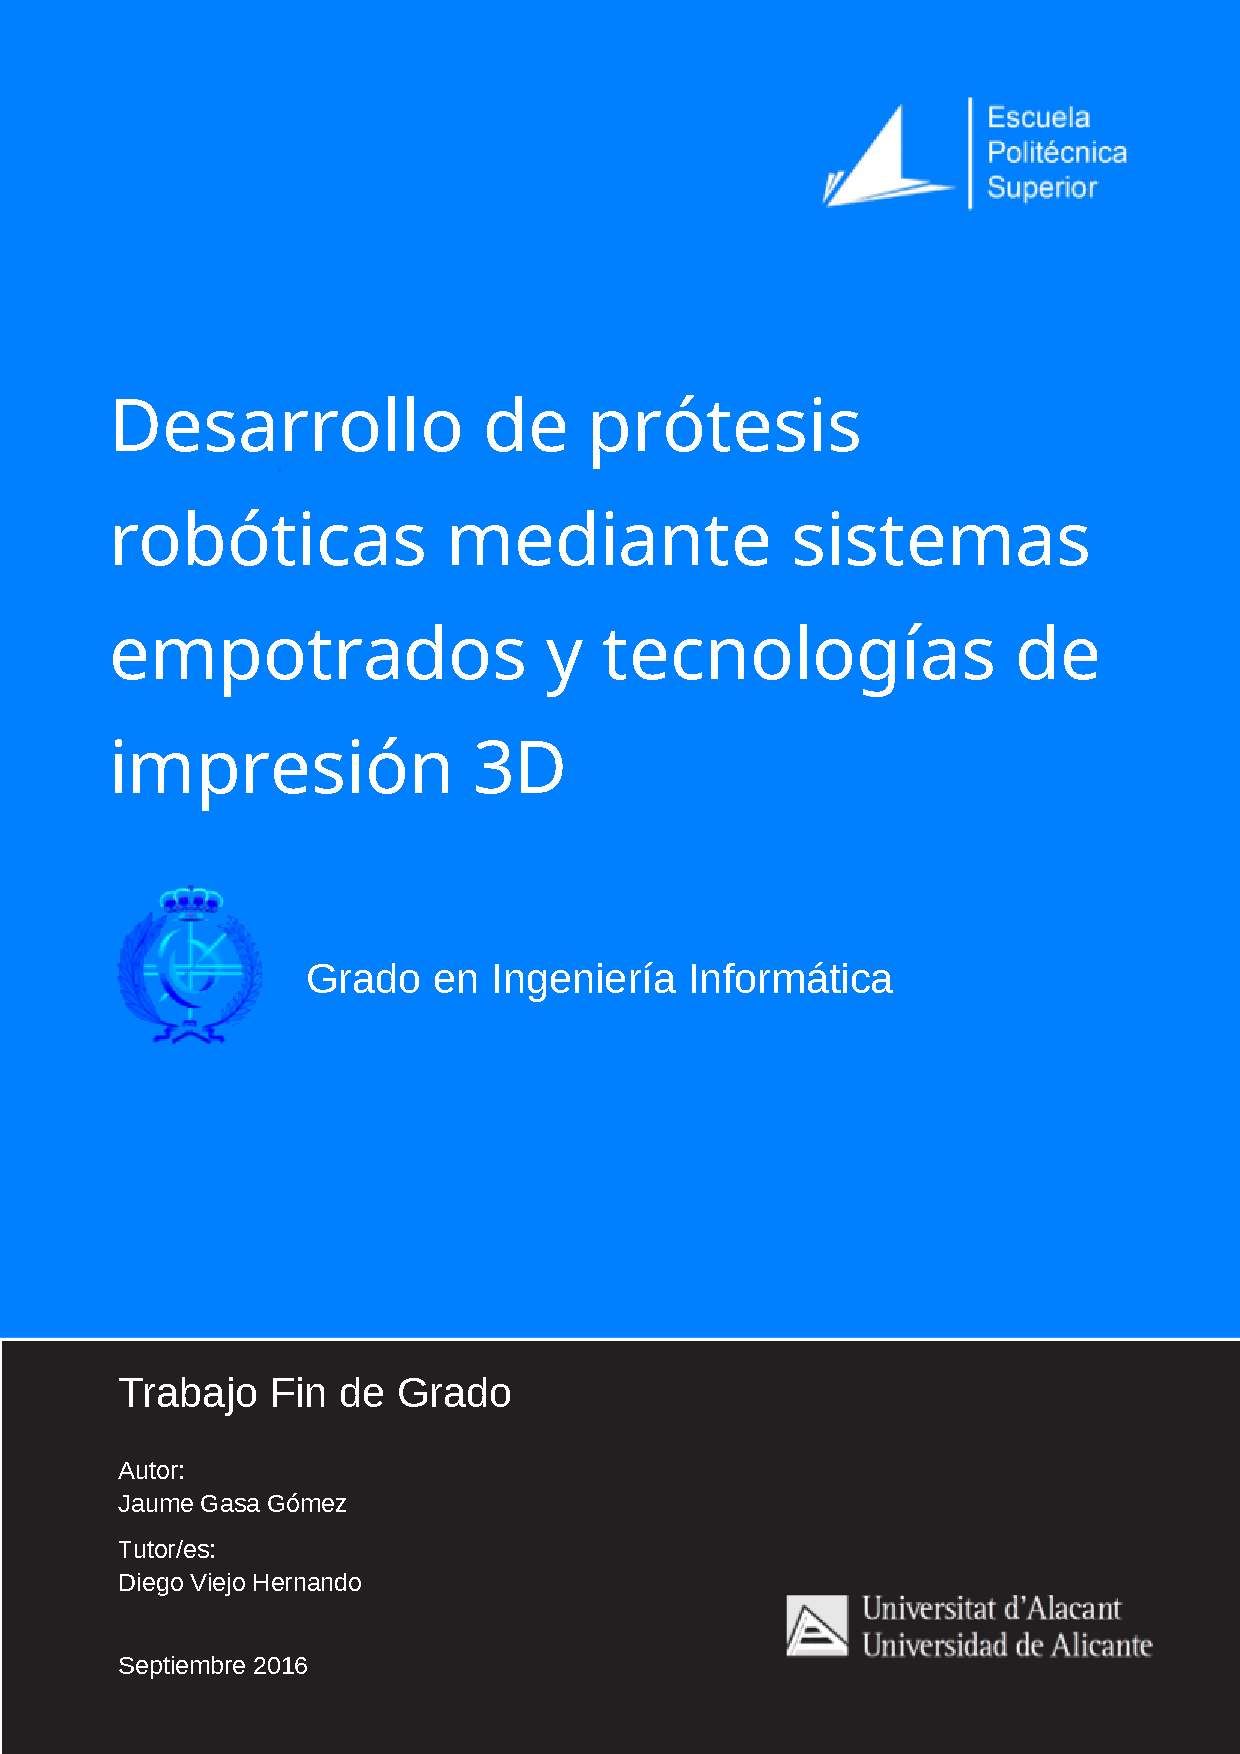
\includepdf[pages=-]{portada.pdf}

\frontmatter % Use roman page numbering style (i, ii, iii, iv...) for the pre-content pages

\pagestyle{plain} % Default to the plain heading style until the thesis style is called for the body content


%----------------------------------------------------------------------------------------
%   ABSTRACT PAGE
%----------------------------------------------------------------------------------------

\begin{abstract}
\addchaptertocentry{\abstractname} % Add the abstract to the table of contents

En este proyecto, se propone realizar una prótesis de miembro superior utilizando técnicas de impresión 3D y sistemas empotrados. Para el control de esta prótesis, se ha desarrollado una red neuronal
artificial, que clasificará las señales leídas mediante ocho sensores mioeléctricos. Mediante este proceso de clasificación se podrá controlar el movimiento de los dedos de la prótesis mediante el uso de
Arduino y un controlador de motores. El proceso de obtención de señales se realizará usando la Myo Armband, que está equipada con ocho sensores EMG, a su vez, para identificar qué longitud corresponde a
cada señal EMG, se utilizará la librería para visión artificial OpenCV con la que se podrá asociar señales EMG a distintas etiquetas que representará cómo de estirado se encuentra el dedo para cada una
de las señales EMG.


\end{abstract}




%----------------------------------------------------------------------------------------
%   LIST OF CONTENTS/FIGURES/TABLES PAGES
%----------------------------------------------------------------------------------------

\tableofcontents % Prints the main table of contents

\listoffigures % Prints the list of figures

\listoftables % Prints the list of tables

\lstlistoflistings



%----------------------------------------------------------------------------------------
%   THESIS CONTENT - CHAPTERS
%----------------------------------------------------------------------------------------

\mainmatter % Begin numeric (1,2,3...) page numbering

\pagestyle{thesis} % Return the page headers back to the "thesis" style

% Include the chapters of the thesis as separate files from the Chapters folder
% Uncomment the lines as you write the chapters


% Chapter Template

\chapter{Introducción} % Main chapter title
\label{Chapter1}

% Objetivos
% énfasis a la importancia de la temática, su vigencia y  actualidad;
% se  planteará  el  problema  a  investigar,  así  como  el  propósito  o
% finalidad de la investigación.

% TODO: Actualizar con los puntos de este capítulo (X.1, X.2) y una descripcion
%mínima
\chapquote{En este capítulo se se detallarán los motivos por los cuales se ha desarrollado este trabajo. En el apartado \ref{sec:outline} se condensan las intenciones del desarrollo de este trabajo. En el apartado \ref{sec:motivación} se explicará punto por punto qué ha determinado elegir este proyecto. El apartado \ref{sec:proyectos_relacionados} se introduce un estado del arte del las prótesis. El apartado \ref{sec:objetivos} se determina cuál se espera que sea el alcanza de este proyecto. Por último, el apartado \ref{sec:estructura}, resume el contenido del trabajo capítulo por capítulo.}




%%%%%%%%%%%%%%%%%%%%%%%%%%%%%%%%%%%%%%%%%%%%%%%%%%%%%%%%%%%%%%%%
%
%
%        Outline
%
%
%%%%%%%%%%%%%%%%%%%%%%%%%%%%%%%%%%%%%%%%%%%%%%%%%%%%%%%%%%%%%%%%

\section{Síntesis}
\label{sec:outline}


The  EMG  signal  is  a  biomedical  
signal   that   measures   electrical   currents   generated   in   
muscles       during       its       cont
raction       representing       
neuromuscular  activities.


Este trabajo consiste en la creación de un sistema, cuyo objetivo es acercar las
prótesis mioeléctricas al público general. Para ello, los esfuerzos se han
centrado en la creación de un modelo protésico mediante impresión 3D, el montaje del
mismo y sus componentes electrónicos, investigación sobre las distintas formas de captar
las señales electromiográficas (estas señales miden las corrientes eléctricas generadas en los músculos durante su contracción \cite{emg}) y la aplicación de algoritmos de aprendizaje artificial para la
clasificación de estas señales. A estos últimos apartados dedicaremos la mayor parte del
esfuerzo de este trabajo, con su posterior evaluación y comparación de los resultados de
cada algoritmo, a fin de constatar si es viable la creación de un sistema que sea robusto
para ser usado \textit{a posteriori}, como base de la creación de una prótesis de
miembro superior mioeléctrica, inteligente y de bajo coste.




%%%%%%%%%%%%%%%%%%%%%%%%%%%%%%%%%%%%%%%%%%%%%%%%%%%%%%%%%%%%%%%%
%
%
%        Motivación
%
%
%%%%%%%%%%%%%%%%%%%%%%%%%%%%%%%%%%%%%%%%%%%%%%%%%%%%%%%%%%%%%%%%

\section{Motivación}
\label{sec:motivación}

Este trabajo surge de la necesidad de dar forma a todos los conocimientos adquiridos
a lo largo de la carrera, así como de aunar y profundizar
en las pasiones descubiertas estos años. Así pues, este proyecto ha sido fuertemente influenciado por:

\begin{itemize}
  \item Parte de inteligencia artificial.
    \begin{itemize}
      \item 34024 - Sistemas Inteligentes.
      \item 34031 - Razonamiento Automático.
      \item 34032 - Desafíos de programación.
      \item 34034 - Procesamiento de Lenguajes.
      \item 34030 - Visión Artificial y Robótica.
    \end{itemize}


  \item Parte de microcontroladores y robótica.
    \begin{itemize}
      \item 34036 - Tecnología y Arquitectura Robótica.
      \item 34049 - Sistemas Embebidos.
      \item 34050 - Sistemas Industriales.
    \end{itemize}

  \item Desarrollo personal.
    \begin{itemize}
      \item Curso CECLEC Taller impresoras 3D REPRAP, \textit{Universidad de
        Alicante}.
      \item Introduction to Computational Thinking and Data Science,
        \textit{Massachusetts Institute of Technology through edX}.
    \end{itemize}
\end{itemize}


Otra necesidad ha sido poder desarrollar y trabajar sobre un prototipo real,
teniendo en mente poder aplicar todos los conocimientos mencionados
anteriormente
sobre éste. Por tanto, la impresión 3D ha tenido un papel fundamental, debido a que el uso
de cualquier otra tecnología para este fin habría sido ineficiente debido a su
alto coste.



\subsection{Motivación social}
\label{sub:Motivación-social}

Según la Asociación Nacional de Amputados (Adampi), se calcula que unas 50.000
personas en España llevan prótesis \cite{mundo-10-barbaridad}, sin contar con las que no han podido
costeárselas o quienes las adquieren por el sector privado. Además, un 10\% del
total son niños en edad de crecimiento \cite{abc-olvidados}.

Una amputación no es solo un problema fisiológico, sino que repercute en la
persona a nivel psicológico, social y económico, por lo que no basta solo con
facilitar ayudas para adquirir una prótesis y esperar que la persona tenga
suficiente dinero para pagar el porcentaje restante o que sea ella quien se
tenga que adaptar a la prótesis y no viceversa.

En esta línea se ha hecho el estudio El impacto emocional de la Ayuda Técnica
(2013), que destaca el ``papel integrador'' de las prótesis para este colectivo
y recoge sus principales demandas, que son:

\begin{itemize}
  \item \textbf{Una prótesis adecuada a las necesidades} : Una prótesis para un
	niño o niña en edad de crecimiento va a necesitar ser sustituida cada poco tiempo
	además de resistente, ya que son susceptibles de romperse cuando éstos/as
	juegan; una persona joven va a necesitar una prótesis funcional y que le
	facilite la integración laboral, y una persona mayor quizá no va a requerir
	una prótesis tan resistente pero sí que se adapte a ella. También habrá que
	valorar el estilo de vida de cada persona para poder ofrecer una prótesis
	adecuada a sus necesidades.

  \item \textbf{Cambiar la visión actual sobre el gasto social}: El gasto social
  	es realmente una inversión, tanto para mejorar el bienestar y la calidad de
	vida de las personas, como para ahorrar futuros gastos derivados de un
	recurso inadecuado. Además, favorece la integración laboral, lo que supone
	una inversión para el Estado y la recuperación del dinero destinado al gasto
	social.

  \item \textbf{Facilitar los procesos de adquisición y/o cambio}: Al tratarse
  	de un proceso parcialmente administrativo, puede resultar lento y complejo.
	Esto dificulta la realización de las actividades diarias así como la
	normalización de la situación de la persona.

\end{itemize}

En España, distintas asociaciones han puesto de manifiesto su disconformidad
sobre el actual sistema de subvenciones que estipula el Real Decreto 1506/2012
aprobado por el Ministerio de Sanidad \cite{boe}. Así, a día de hoy, muchas familias tienen
que pagar el 10\% de las prótesis, lo que puede suponer 3000\euro~en algunos casos,
sin tener en cuenta que, como ya hemos comentado, se deben renovar cada pocos
años en el caso de niños y niñas. Por otro lado, las prótesis no han sufrido un
proceso de evaluación y mejora, por lo que han quedado obsoletas o
desactualizadas; sin embargo, los precios actuales son los estipulados por este
decreto en el año 2012, que son elevados para el nivel de calidad de vida que
aportan.


En cuanto al aspecto psicológico, es sabido que las personas con amputaciones
tienen dificultades para la participación e integración social. Estas personas
se pueden encontrar con falta de autonomía para realizar tareas básicas,
frustración e incluso aislamiento social. El hecho de que puedan contar con una
prótesis de calidad y adaptada a su condición supone un impacto emocional
positivo que facilita que la persona vuelva a tener confianza en sí misma y
aumente su bienestar social y emocional y su calidad de vida.

Todo esto es lo que ha motivado la realización de este proyecto que, en
definitiva, pretende solventar estos problemas mediante el desarrollo de una
prótesis mioeléctrica impresa en 3D que ofrece un modelo funcional y
actualizado, para el que se necesita un bajo coste de producción, lo que
repercutirá en el precio final de mercado, que será menor que el actual y por
tanto podrá facilitar su adquisición a más personas. Asimismo, se han utilizado
tecnologías libres para que las personas interesadas puedan aportar ideas y/o mejoras a este proyecto.




%%%%%%%%%%%%%%%%%%%%%%%%%%%%%%%%%%%%%%%%%%%%%%%%%%%%%%%%%%%%%%%%
%
%
%        Proyectos relacionados
%
%
%%%%%%%%%%%%%%%%%%%%%%%%%%%%%%%%%%%%%%%%%%%%%%%%%%%%%%%%%%%%%%%%

\section{Proyectos relacionados}
\label{sec:proyectos_relacionados}

Como veremos a continuación, existen diversos proyectos, que se han desarrollado
en los últimos años en el ámbito de las prótesis. Esto es debido, en gran parte,
al denominado movimiento \textit{maker} y al cada vez más fácil acceso de las
impresoras 3D por parte del público general.

En las siguientes subsecciones, se hará un repaso de los proyectos que se
están desarrollando actualmente, con el fin de contextualizar las diversas
técnicas empleadas en este trabajo en el sector de las prótesis de miembro
superior.


%-----------------------------------
%	SUBSECTION 1
%-----------------------------------
\subsection{Automail}
\label{sub:automail}

Proyecto hecho público recientemente \cite{enable-myo} (25 marzo de 2016)
que comparte algunos componentes con los de este trabajo. Consiste en una
aplicación python diseñada para ser cargada en una Raspberry Pi \cite{raspberry-pi}
y que actúa de puente entre la Myo Armband~\ref{subs:myo} y un Arduino~\ref{subs:arduino}.

El funcionamiento \cite{automail} consiste en sincronizar la Myo Armband con una Raspberry Pi y
ésta a un Arduino, que se encargará de girar una base conectada a un motor
servo, el cual hará girar la prótesis sobre su eje z. El giro hacia la izquierda
o derecha depende de si la mano está abatida haca dentro o fuera
respectivamente.

Por otra parte, es capaz de mandar una señal a la prótesis si se cierra el puño
para agarrar objetos o de soltarlo si se separan los dedos.

\begin{figure}[h]
    \centering
    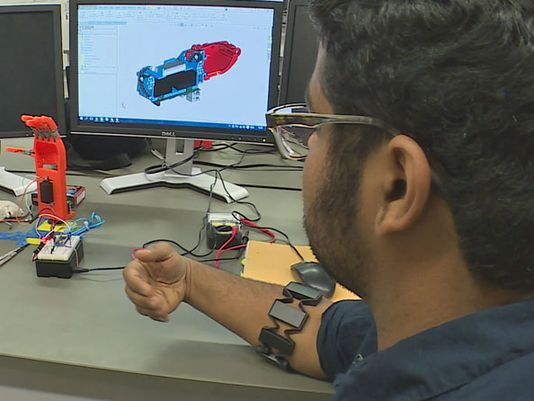
\includegraphics[width=0.7\textwidth]{Chapter1/automail}


\caption{Muestra del proyecto Automail en acción. Figura extraida de legacy.king5.com}
%http://legacy.king5.com/story/tech/science/2015/10/13/students-develop-technology-to-make-prosthetics-more-affordable/73901962/
\label{fig:automail}
\end{figure}


Este proyecto destaca por la correcta integración de los distintos
componentes (Myo, Raspberry Pi y Arduino). No obstante, al no estar
especificado,
se entiende que el proceso de reconocimiento de poses es el que viene
implementado por defecto en la Myo, el cual, al actuar como caja negra, es
imposible saber cómo funciona y, mucho menos, poder modificarlo para nuestras
necesidades.



%-----------------------------------
%	Inmoov
%-----------------------------------
\subsection{Inmoov}
\label{subs:inmoov}

Inmoov nace como proyecto personal de Gael Langevin, con el objetivo de crear
un robot humanodide hecho con tecnología de impresión 3D, completamente
funcional y libre \cite{langevin2014inmoov}. La relación con este proyecto surge
del uso que le ha dado la comunidad, ya que, al ser libre, se ha decidido utilizar
el brazo (Figura~\ref{fig:inmoov}) como prótesis.

\begin{figure}[htp]
  \centering
    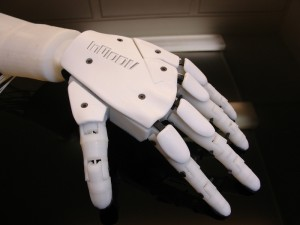
\includegraphics[width=0.8\textwidth]{Chapter1/inmoov}
  \caption{Mano y parte del brazo del proyecto Inmoov.}
\label{fig:inmoov}
\end{figure}

Inmoov destaca por su documentación sobre la construcción de la mano, que lo ha hecho
relativamente popular. Por contrapartida, el proyecto tiene un caracter
más conceptual que %TODO: rellenar esta parte y revisar todo este párrafo,
siendo habitual verlo como parte de exposiciones en museos y en algunas ferias
tecnológicas. Esto, aunque pueda parecer que no es una gran inconveniencia, en
la práctica se está viendo cómo nuevas versiones de la mano y el antebrazo están
dejando de ser 100\% libres. Por parte de la comunidad se ve bastante
actividad, pero no documentada, por lo que son simples bancos de pruebas sin desarrollar
aplicaciones serias.



%-----------------------------------
%	Open Bionics
%-----------------------------------
\subsection{Open Bionics}
\label{sub:open-bionic}

Conocida anteriormente como Open hand project, es una empresa incubada en el
Laboratorio de Robótica de Bristol que tiene como objetivo la creación de
prótesis de mano impresas en 3D y de bajo coste \cite{remenyi2015innovation}.
Este proyecto ha participado en distintas competiciones, donde destaca
el 2º puesto en Make it wereable de Intel 2014 y el 1º puesto en Innovación en
ingeniería
de los premios James Dyson 2015. Estos premios, entre otros, han permitido
que el proyecto siga desarrollándose. Actualmente, están trabajando
con la prótesis Ada (Figura~\ref{fig:ada}), así como su propio
microcontrolador PCB, el Almond PCB.
% TODO: incluir acrónimo PCB



\begin{figure}[htp]
  \centering
    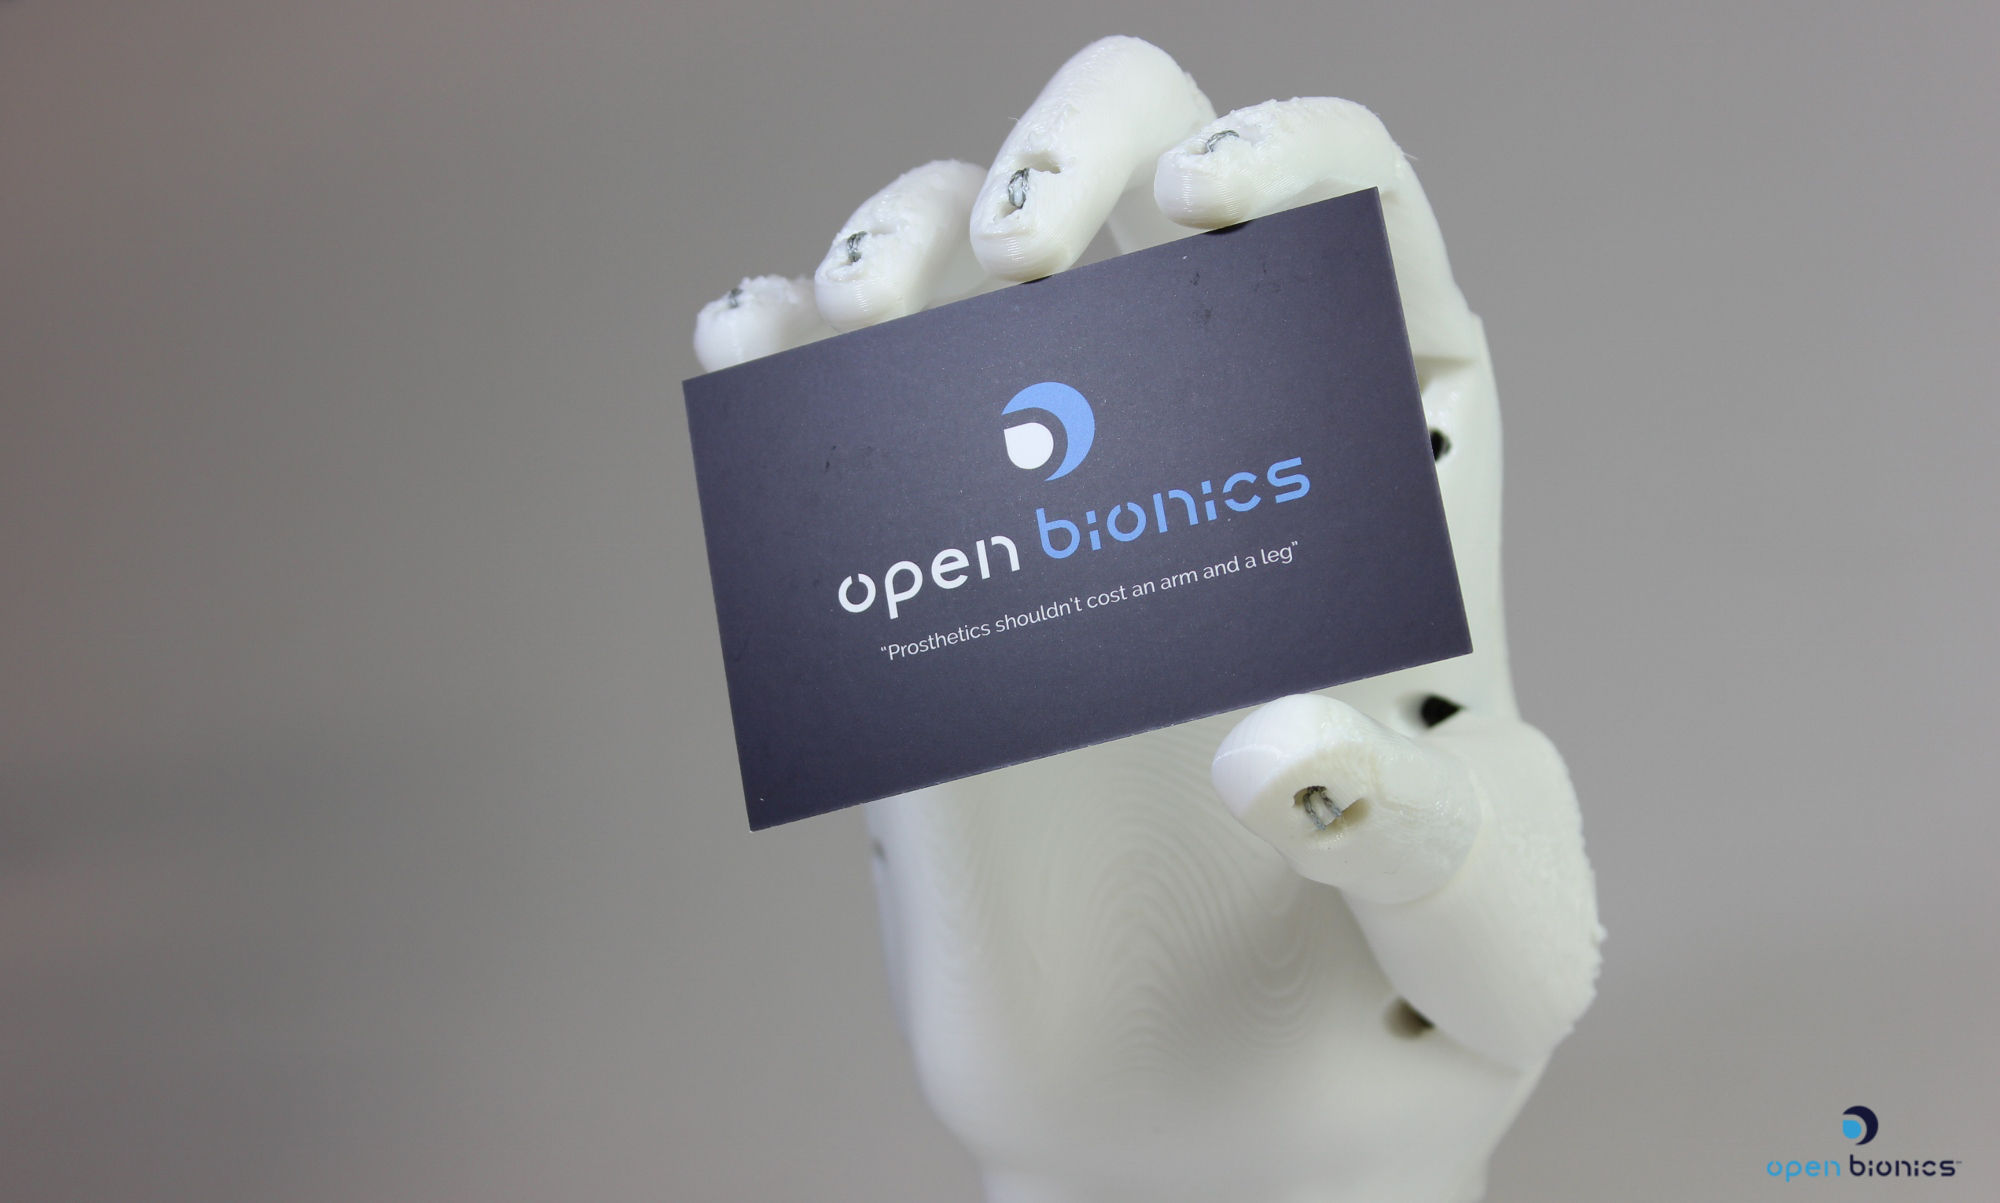
\includegraphics[width=0.8\textwidth]{Chapter1/ada}
  \caption{Ada, el último modelo de prótesis desarrollado por Open Bionics.}
\label{fig:ada}
\end{figure}


El modelo Dextrus, anterior a Ada, fue desarrollado en los inicios de esta
empresa
como parte del proyecto Open hand project. En la figura~\ref{fig:dextrus} se
muestra
una mano impresa basada en los modelos 3D Dextrus.


\begin{figure}[htp]
  \centering
    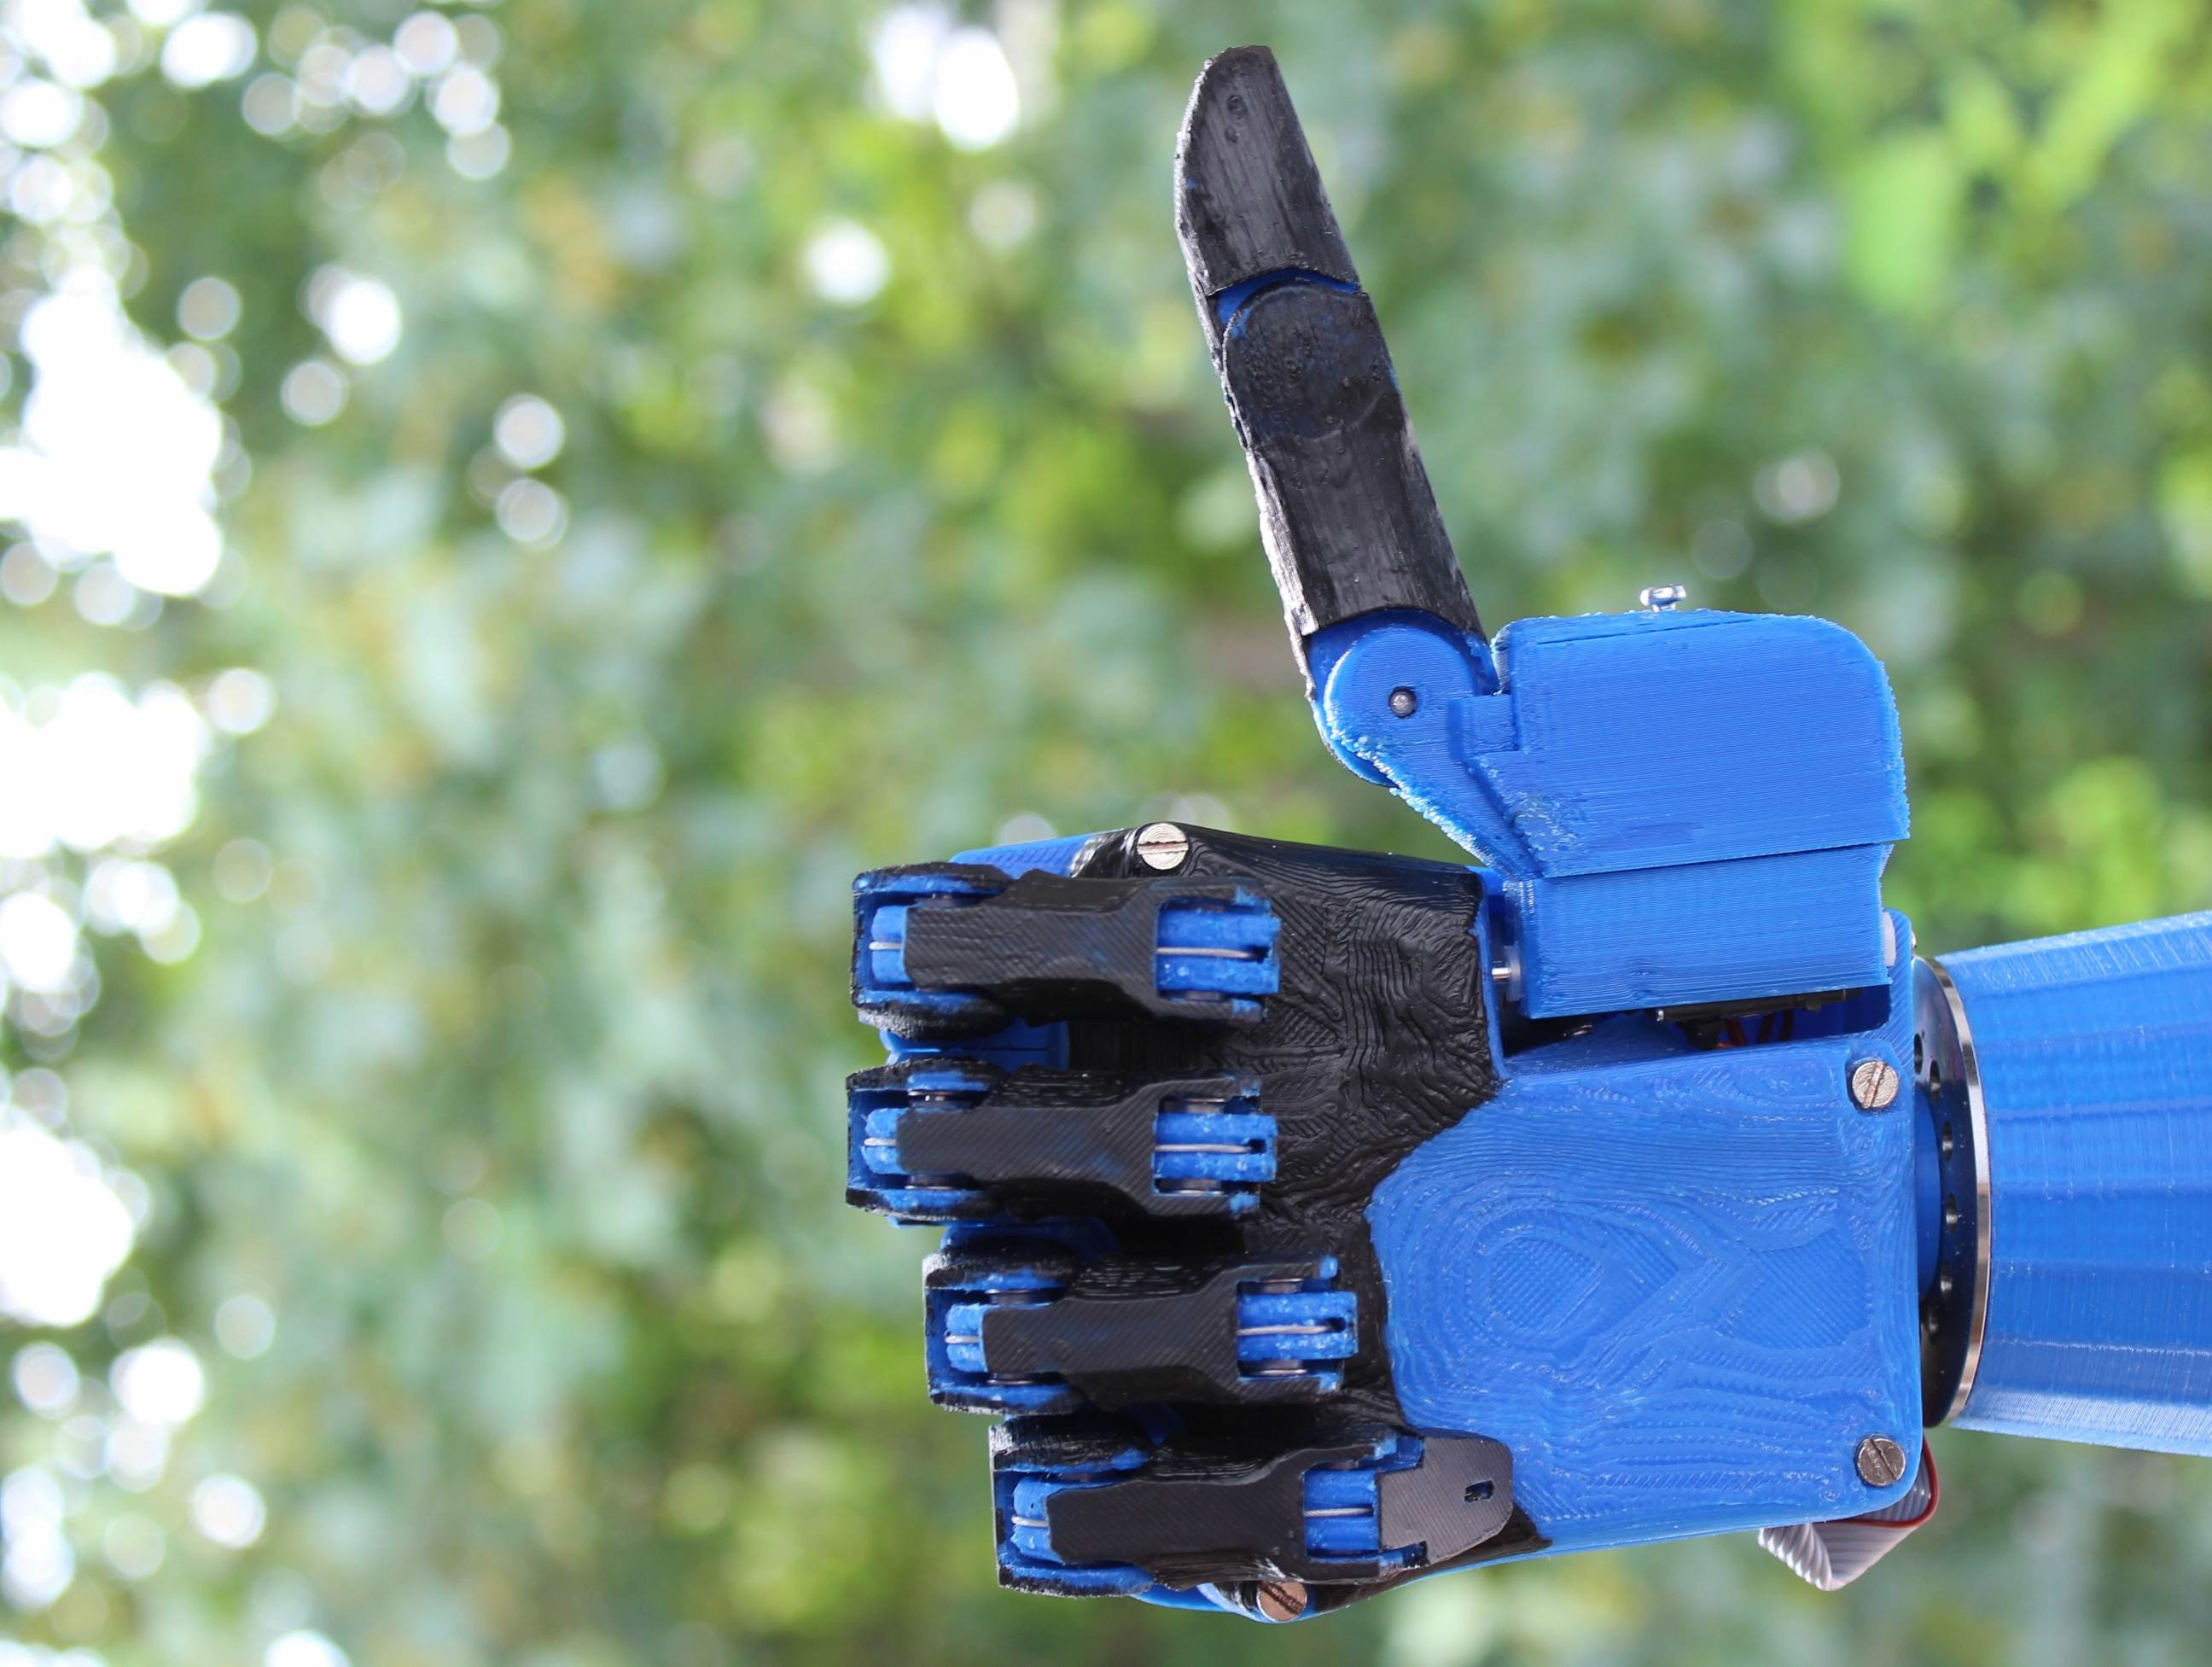
\includegraphics[width=0.65\textwidth]{Chapter1/dextrus}
  \caption{Prótesis Dextrus con el pulgar levantado.}
\label{fig:dextrus}
\end{figure}

%TODO: terminar apartado de OB con la conclusión


\subsection{Bebionic}
\label{sub:bebionic}

La prótesis mioeléctrica de mano Bebionic está diseñada por la empresa
RSLSteeper.
Esta prótesis viene preprogramada con múltiples posiciones de agarre y es
controlada
por la contracción de los músculos, como la mayoría de prótesis mioeléctricas
\cite{medynski2011bebionic}.

Esta prótesis, como se puede apreciar en al figura~\ref{fig:bebionic}, se
caracteriza por usar los materiales y técnicas más avanzadas actualmente. Es capaz de
realizar 14 posiciones o patrones de agarre distintos, además de poder usar el
pulgar de forma abatible (que ha de accionarse manualmente). La electrónica se
encarga de realizar una monitorización de cada motor (uno por cada dedo) para
reproducir correctamente los patrones y maximizar la precisión de cada
movimiento \cite{medynski2011bebionic}.


\begin{figure}[htp]
  \centering
    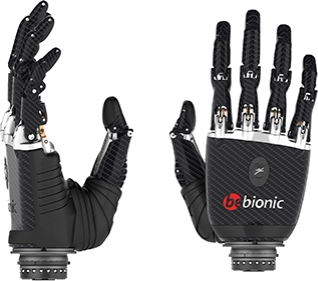
\includegraphics[width=0.6\textwidth]{Chapter1/bebionic}
  \caption{Perfil y reverso de Bebionic}
\label{fig:bebionic}
\end{figure}

% TODO: añadir RF a acrónimos (radiofrequencia)

El software que acompaña esta prótesis es Bebalance desarrollado por la propia
RSLSteeper. Toda la información es transmitida desde y hacia este sistema
mediante un emisor y receptor RF incorporado en la prótesis
\cite{waryck2011comparison}.
Bebalance permite, entre otras cosas, la configuración de la presión que puede
ejercer o la velocidad de los motores. Es posible también realizar un
seguimiento visual de los sensores mediante monitores de análisis en tiempo
real, permitiendo al usuario practicar mediante un \textit{feedback} real de
los sensores \cite{medynski2011bebionic}.

RSLSteeper autodenomina esta prótesis como ``La prótesis de mano más avanzada
del mundo'' \cite{bebionicWeb}. Por ello, y por su precio, que oscila entre
los 25.000\$ y los 35.000\$ \cite{bebionicPrice}, se ha tomado como cota
máxima
de lo que una prótesis, actualmente, puede hacer y qué limitaciones tiene.



\subsection{Propósitos}
\label{sub:propósitos}

Después de entender la motivación de este TFG y conocer el estado de desarrollo de los proyectos
relacionados que se están llevando a cabo hasta el momento, este trabajo pretende lograr:

\begin{itemize}
  \item Reducción del coste final de una prótesis de mano mioeléctrica.
  \item Crear un sistema de detección de patrones robusto.
  \item Los movimientos de la prótesis deben adecuarse de forma realista a las
  acciones hechas por el usuario.
  \item Facilitar el uso y configuración de la prótesis a usuarios no expertos.
  %TODO revisar penúltimo punto
\end{itemize}


\section{Objetivos}
\label{sec:objetivos}


El objetivo final es que una prótesis impresa en 3D sea capaz de reproducir
el movimiento natural de una mano real. Estos movimientos han de ser la respuesta a los impulsos
eléctricos del músculo del usuario, que son captados mediante un dispositivo
con sensores de señales EMG (siglas para electromiografía).

El proceso de identificación de qué movimiento debe realizar la prótesis será
implementado usando técnicas de inteligencia artificial, más concretamente,
algoritmos de clasificación.

% TODO: indicar la sección o capítulo
El proceso de aprendizaje, como veremos más adelante en \ref{sec:clasificación-señales-emg},
requiere una gran cantidad de colección de datos de todos los movimientos que se quieren
reproducir, por lo que, teniendo en cuenta que cada usuario será distinto, se facilitará una
forma lo más sencilla posible de obtener la cantidad de datos necesaria que
se precise para el correcto funcionamiento del proceso de clasificación.

Para asegurar que el sistema final sea robusto, se especificarán distintos
movimientos y se recopilarán los conjuntos de datos necesarios para aplicar distintos
algoritmos, así como distintas técnicas para decidir de forma objetiva qué algoritmo
funciona mejor con el tipo de dato que proporciona el dispositivo EMG y que será empleado
en el producto final.

Por último, aunque todo el proceso de desarrollo del sistema se haga en forma
de prototipo, se deberá realizar un análisis de la viabilidad de la exportación
del trabajo a un entorno real, es decir, estimar la vida útil de la prótesis con
las baterías actuales disponibles o comprobar si el precio de los componentes
necesarios para un entorno real no superan los límites para que la prótesis siga
considerándose de bajo coste.


\section{Estructura}
\label{sec:estructura}

Este TFG se ha estructurado de la siguiente forma:

\begin{itemize}
	\item Capítulo \ref{Chapter1}: se resume el proyecto y los motivos por el que se ha desarrollado. Se incluye también, un estado del arte sobre las prótesis y proyectos más destacables sobre las mismas.
	\item Capítulo \ref{Chapter2}: aúna las herramientas utilizadas para el desarrollo de la prótesis y de su sistema de control.
	\item Capítulo \ref{Chapter3}: introducción a los algoritmos de aprendizaje automáticos, con especial hincapié en  los modelos de redes neuronales artificiales.
	\item Capítulo \ref{Chapter4}: descripción de los métodos desarrollados para la obtención del conjunto de datos que será utilizado a su vez, por el modelo de aprendizaje para clasificar las señales EMG.
	\item Capítulo \ref{Chapter5}: conclusiones sobre los resultados obtenidos y propuestas para continuar y mejorar el trabajo realizado.
\end{itemize}

% Chapter Template

\chapter{Metodología} % Main chapter title
\label{Chapter2}



%\chapquote{En este capítulo se incluye una breve descripción de distintos proyectos que han
%influenciado el desarrollo de este Trabajo de Fin de Grado. En la sección \ref{sec:automail}
%el proyecto combina Myo, Raspberry Py y Arduino para realizar movimientos simples en una
%prótesis.}

\chapquote{En este segundo capítulo, se hablará de los distintos elementos que
conforman la tesis. En apartado~\ref{sec:introducción2} se dará un breve resumen.
A continuación, el apartado~\ref{sec:tecnologías} hablará tanto de los
componentes software como hardware que han sido utilizados. Por último, el apartado \ref{sec:prótesis-electrónica} muestra el entorno de trabajo real.}

% TODO: http://ieeexplore.ieee.org/xpl/login.jsp?tp=&arnumber=5670617&url=http%3A%2F%2Fieeexplore.ieee.org%2Fxpls%2Fabs_all.jsp%3Farnumber%3D5670617
% TODO: http://ieeexplore.ieee.org/xpl/login.jsp?tp=&arnumber=6361492&url=http%3A%2F%2Fieeexplore.ieee.org%2Fxpls%2Fabs_all.jsp%3Farnumber%3D6361492


\section{Introducción}
\label{sec:introducción2}

%Este capítulo aportará información respecto a cómo se ha elaborado el trabajo.
%El proyecto de esta tesis pretende ser un proyecto, por lo cual se ha requerido
%no solo del estudio e investigación de otros proyectos, sino que se ha tenido
%que desarrollar de forma práctica. Por ello, en el subapartado \ref{sec:tecnologías}
%se explicará algunos recursos utilizados para el desarrollo del proyecto.

%TODO completar con lo que se desarrolle más adelante

Debido a la amplitud del proyecto, en este capítulo se pretende dar un repaso a todas las herramientas utilizadas así como una breve descripción de las mismas y por qué han sido elegidas. Por una parte, en el subapartado \ref{sub:software} se describen las herramientas utilizadas para desarrollar el modelo de aprendizaje que controlará la prótesis, además se incluye una descripción de los programas utilizados para poder imprimir los modelos 3D de la prótesis en la impresora 3D (en \ref{subs:prusa-i3} se describe la impresora utilizada). Por otra parte, el subapartado \ref{sub:hardware}, contiene tanto la descripción de las herramientas físicas utilizadas, es decir, todos los sensores, cotroladores y la propia impresora 3D anteriormente citada. Por último, el apartado \ref{sec:prótesis-electrónica} describe más en profundidad el funcionamiento de la prótesis y sus componentes electrónicos.



\section{Tecnologías}
\label{sec:tecnologías}

En este apartado se aportará información tanto del \textit{software},
subapartado~\ref{sub:software}, como del \textit{hardware}, subapartado~\ref{sub:hardware},
empleado para el desarrollo del proyecto.


\subsection{Software}
\label{sub:software}

La parte \textit{software} del proyecto recae sobre la implementación de algoritmos de
aprendizaje automático y la comunicación entre los diferentes componentes
(descritos en el subapartado~\ref{sub:hardware}). De forma adicional, se
añadirá de forma breve los programas necesarios para la impresión de la prótesis.

%TODO: mencionar python y git como subsubapartado o como párrafo aqui?


\subsubsection{Scikit-learn}
\label{subs:scikit-learn}

%TODO: añadir SVM a los acrónimos

Scikit-learn \cite{scikit-learn} es un módulo de Python que integra un gran
número de algoritmos de aprendizaje automático para problemas de tamaño medio de
clasificación y regresión.

\begin{figure}[htp]
  \centering
    
\includegraphics[width=0.4\textwidth]{Chapter2/scikit-learn}
  \caption{Logo de Scikit-learn}
\label{fig:scikit-learn}
\end{figure}

 El módulo cuenta con la librería de C++ LibSVM y
LibLinear para la implementación de SVM y modelos lineales generalizados. Está
construido además sobre \textit{numpy}, que proporciona la estructura base de
los datos y el modelo de parámetros; \textit{Scipy}, que aporta algoritmos
eficientes para álgebra lineal, representación de matrices dispersas y funciones
de estadística básica; y por último \textit{Cython}, un lenguaje que combina
\textit{C} y \textit{Python} para obtener el rendimiento de los lenguajes
compilados, con la sintaxis y las operaciones de un lenguaje de alto nivel como
\textit{Python}.

Como la mayoría del ecosistema Python, Scikit-learn está distribuido mediante
una licencia BSD, lo que permite su uso en proyectos comerciales, que a su vez,
contribuyen a mantener el desarrollo del proyecto. Algunas de las empresas que
usan Scikit-learn son Spotify y Evernote \cite{scikit-learn-empresas}.

Se ha elegido este proyecto para la clasificación de las poses por la versatilidad
y rapidez de desarrollar prototipos, la vigencia y eficiencia de los algoritmos
que implementa. Además aporta en su documentación toda la base matemática y
explicaciones del funcionamiento de los algoritmos, es decir, no solo aporta
información acerca de como usar los algoritmos en Python, sino también su base
teórica.


\subsubsection{Theano}
\label{subs:theano}

\begin{figure}[htp]
  \centering
    
\includegraphics[width=0.4\textwidth]{Chapter2/theano}
  \caption{Logo de Theano}
\label{fig:theano}
\end{figure}


Theano es la librería que utilizan como base la mayoría de \textit{frameworks} orientados al \textit{deep learning} 
en \textit{Python} \cite{theano-based-projects}. Su uso permite definir, optimizar y evaluar expresiones matemáticas 
mediante \cite{theano}:

\begin{itemize}

	\item Uso de compiladores como \textit{g++} o \textit{nvcc} para optimizar la velocidad de ejecución.
	\item Diferenciación simbólica para construir grafos simbólicos para computar gradientes automáticamente.
	\item Reconocimiento de (algunas) expresiones numéricas inestables. 
	\item Soporte de operaciones dispersas, tensores y álgebra lineal.
	\item Ejecución en paralelo (SIMD, multinúcleo y multinodo en cluster o distribuido).

\end{itemize}


\subsubsection{Lasagne}
\label{subs:lasagne}

Lasagne es una librería ligera para construir y entrenar redes neuronales en theano de forma simple, transparente (no abstrae las expresiones de Theano) y modular~\cite{lasagne}. Sus principales características son:

\begin{itemize}

	\item Permite implementar redes prealimentadas como redes neuronales convolucionales, redes neuronales recurrentes y combinaciones de cualquier modelo de las redes mencionadas.
	\item Permite arquitecturas de cualquier número de entradas y salidas, incluso clasificadores auxiliares.
	\item Uso de métodos de optimización como \textit{Nesterov momentum}, \textit{RMSprop} y \textit{ADAM}.
	\item Uso de CPU y GPU mediante el uso del compiladore de expresiones de Theano.
\end{itemize}



\subsubsection{Nolearn}
\label{subs:nolearn}

Nolearn \cite{nolearn} es un conjunto de \textit{wrappers} y abstraciones de distintas librerías de redes neuronales (principalmente Lasagne) cuya principal característica, y motivo por el que se ha utilizado en este trabajo, es que todo el código es compatible con \textit{Scikit-learn}. El uso de esta librería permite construir una red neuronal y que sea reconocido como un modelo de \textit{Scikit-learn} pudiendo usar cualquier implementación auxiliar de esta librería como si la red neuronal fuera un modelo nativo.

Para mantener la compatibilidad existen ciertas pautas que se han de seguir para desarrollar las redes neuronales. La implementación puede verse en el apartado \ref{nn-arquitecture}



\subsubsection{Myo-raw}
\label{subs:myo-raw}

Proyecto independiente y libre que aporta una interfaz para poder comunicarse
con el dispositivo EMG Thalmic Myo, mediante la posibilidad de poder escanear
y conectarse al dispositivo más cercano, pudiendo de esta forma, acceder a los
datos de los sensores \cite{myo-raw}.

En concreto, este proyecto incluye los siguientes ficheros \textit{.py}:
\textit{myo\_raw.py} provee el acceso a los datos EMG, mediante la clase
MyoRaw, el cual implementa el protocolo de comunicación con la Myo.
\textit{classify\_myo.py}, contiene un ejemplo básico de clasificación, en este
fichero implementaremos nuestros propios algoritmos, mediante la librería scikit-learn,
descrita en el subsubapartado~\ref{subs:scikit-learn}). Por último, \textit{myo.py},
esta clase puede ser usada para notificar a otros programas cuando una pose se ha
``activado''.

A pesar de ser un programa relativamente pequeño, provee las operaciones más importantes
a la hora de trabajar con la \textit{Myo Armband}, sin depender de los SDK
oficiales de la propia empresa, que ha dejado claro su negación (por el momento)
de abrir su producto para poder utilizarlo sin restricciones \cite{myo-close}.
Por ello ha sido la opción elegida para la comunicación entre el el programa que
obtendrá los datos de los sensores EMG de la Myo y que usará el sistema \textit{software}
tanto para el entrenamiento de los algoritmos como para la clasificación de las
poses.


\subsubsection{OpenCV}
\label{subs:opencv}

\begin{figure}[htp]
  \centering
    
\includegraphics[width=0.2\textwidth]{Chapter2/opencv}
  \caption{Logo de la librería OpenCV}
\label{fig:opencv}
\end{figure}

OpenCV (\textit{Open Source Computer Vision}, visión artificial de código abierto) es una librería que contiene 
funciones para trabajar con visión artificial en tiempo real. Es multiplataforma (funciona en Windows, GNU/Linux,
Mac OS, Android e IOS), tiene interfaces para trabajar en C++, C, Python y Java. Su licencia BSD \cite{bsd},
permite su uso tanto 
académico como comercial \cite{opencv}.

Se ha utilizado esta librería por su facilidad de uso mediante la interfaz de Python y la gran cantidad de 
documentación y trabajos disponibles \cite{opencv-python}.




\subsubsection{Cura}
\label{subs:cura}


\begin{figure}[htp]
  \centering
    
\includegraphics[width=0.2\textwidth]{Chapter2/cura}
  \caption{Logo del software Cura de Ultimaker}
\label{fig:cura}
\end{figure}


Cura es un software desarrollado por Ultimaker que permite generar ficheros
\textit{.gcode} (que marca el recorrido que debe realizar la impresora para imprimir correctamente el objeto) a partir de ficheros \textit{.stl} (estos ficheros son exportados desde el programa de diseño con el que se ha realizado el modelaje 3D del objeto), permitiendo configurar todo tipo de parámetros que determinaran la calidad y modo de impresión de la pieza en formato \textit{stl} aportada \cite{Cura}. Cura es distribuido mediante
licencia AGPLv3.



\begin{figure}[htp]
  \centering
    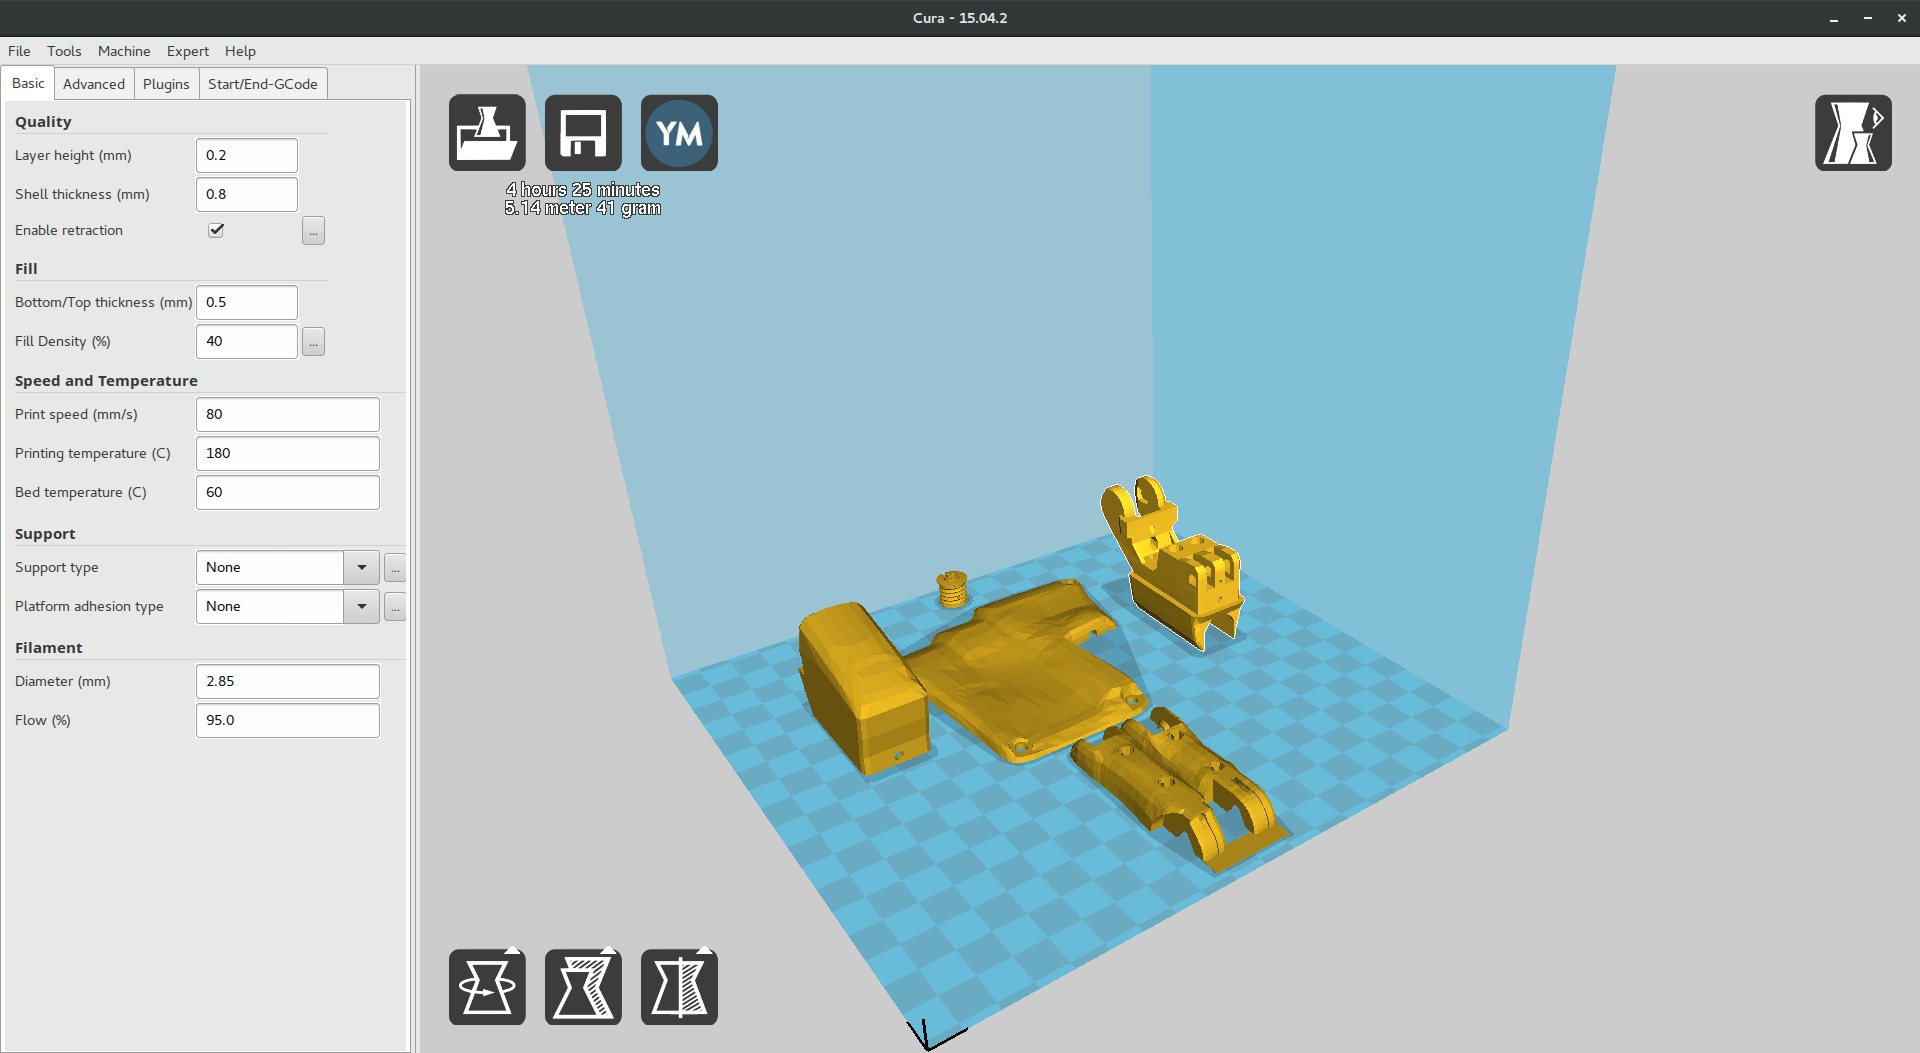
\includegraphics[width=1\textwidth]{Chapter2/cura-desk}
  \caption{Software Cura con algunas partes de la prótesis Dextrus.}
\label{fig:cura-desk}
\end{figure}

Su facilidad de uso y la gran cantidad de opciones que ofrece para la configuración
del proceso de impresión hacen de este programa una herramienta indispensable para
usuarios básicos y avanzados.



\subsubsection{Printrun}
\label{subs:printrun}

Printrun es una colección de programas y scripts que implementa la comunicación
del PC con las impresoras 3D. Está compuesto principalmente por: \textit{printcore.py}
es una librería que permite escribir \textit{reprap hosts}  de forma sencilla;
\textit{pronsole.py} es un programa interactivo con autocompletado basado en comandos;
y, por último, \textit{pronterface.py}, una interfaz gráfica para \textit{pronsole}
\cite{printrun}.

\begin{figure}[htp]
  \centering
    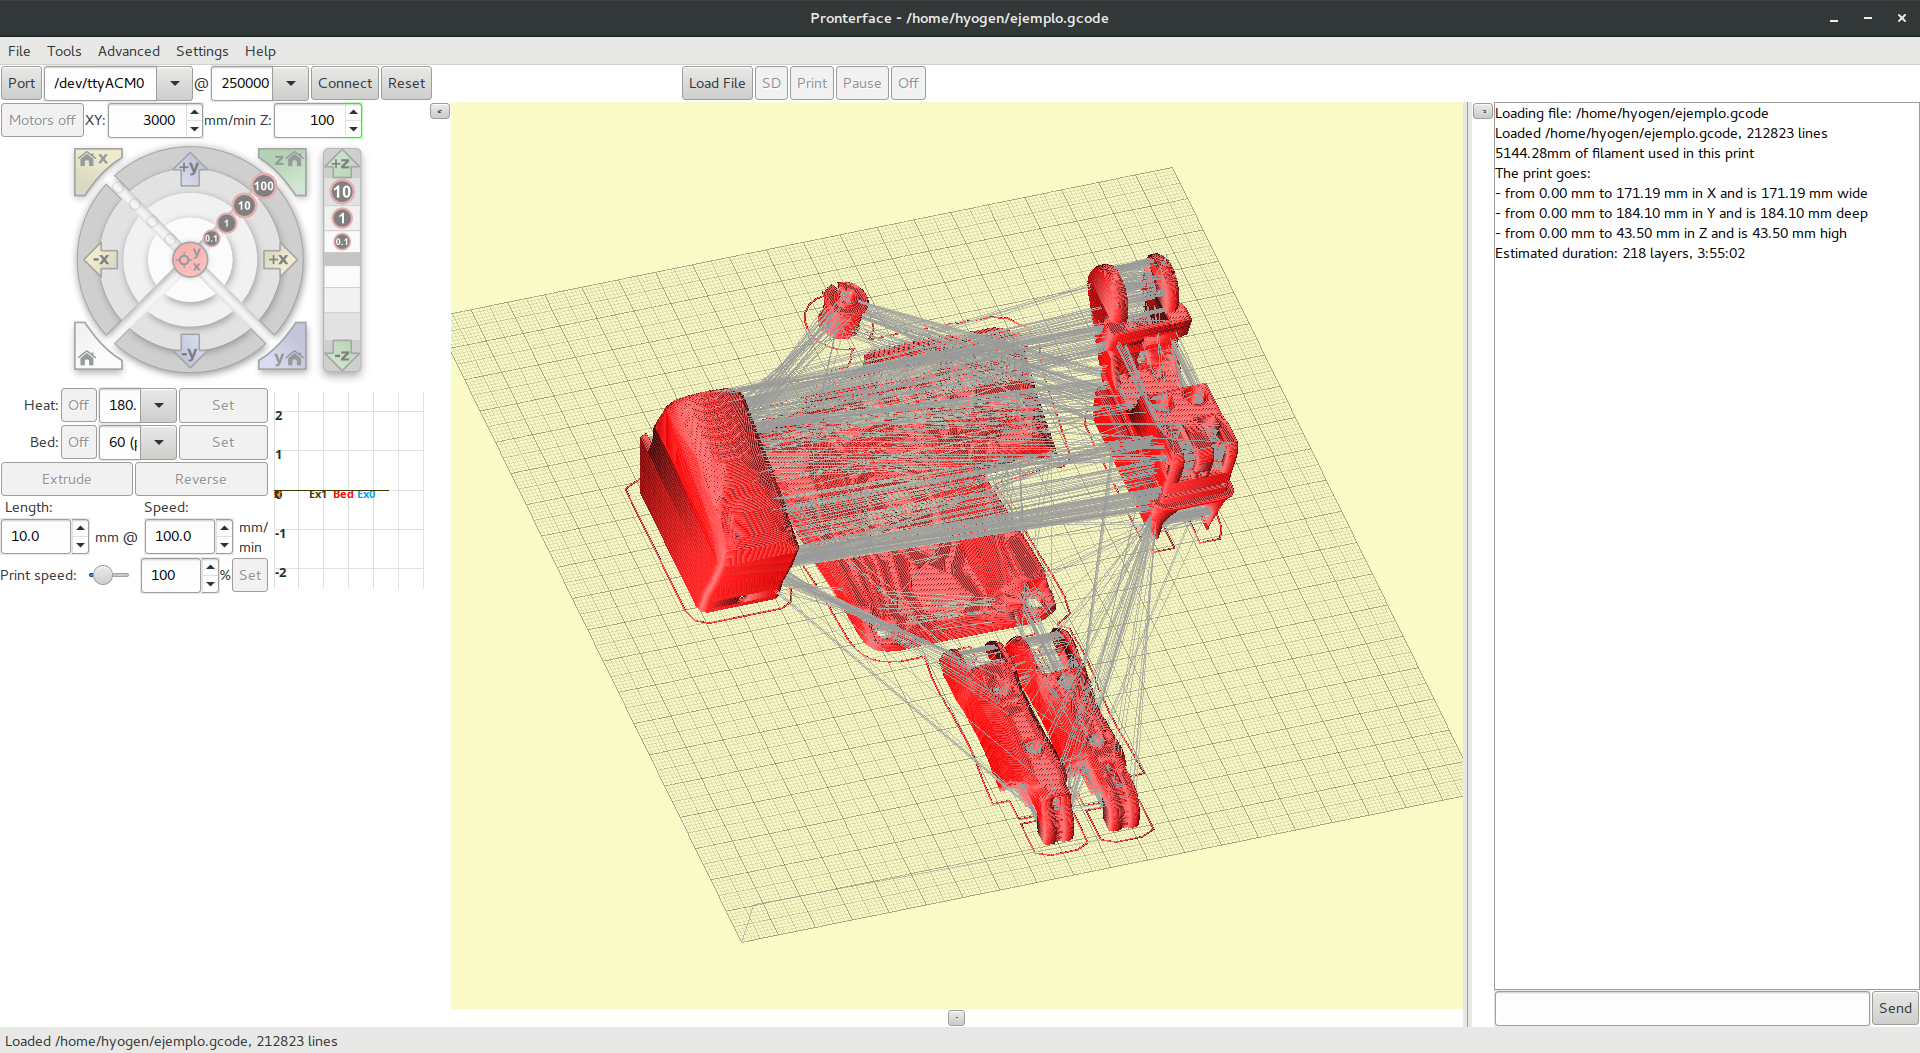
\includegraphics[width=1\textwidth]{Chapter2/pronterface-desk}
  \caption{Pronterface con el gcode cargado de la figura~\ref{fig:cura-desk}.}
\label{fig:pronterface-desk}
\end{figure}

Printrun es el estándar \textit{de facto} para la comunicación entre el PC y la
impresora 3D.



\subsubsection{Arduino IDE}
\label{subs:arduino_ide}

Este software permite desarrollar código para la plataforma \textit{hardware}
Arduino (se describirá en~\ref{subs:arduino}), además de proporcionar la
comunicación entre el ordenador y el microcontrolador, siendo imprescindible
para cargar el código en las placas Arduino. Este \textit{software} está basado
en \textit{Java} y \textit{Processing} y es distribuido mediante la licencia
GPL \cite{arduino-software}.

\begin{figure}[htp]
  \centering
    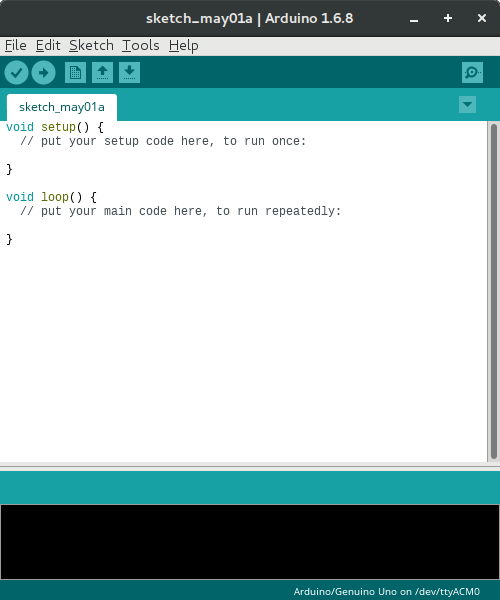
\includegraphics[width=0.7\textwidth]{Chapter2/arduino-ide}
  \caption{Interfaz gráfica del Arduino IDE.}
\label{fig:arduino-ide}
\end{figure}

El IDE de Arduino permite gestionar librerías y cargar de modo sencillo el
\textit{software} desarrollado en los Arduino, por ello, el código se ha escrito
usando este IDE.






\subsection{Hardware}
\label{sub:hardware}

\subsubsection{Arduino}
\label{subs:arduino}

Arduino, figura~Figure~\ref{fig:arduino}  es una plataforma de prototipado libre. Estas placas, permiten leer
datos de entrada (actividad en un sensor, accionado de un botón o un mensaje
de Twitter) y convertirla en un dato de salida (activar un motor, encender
un LED o publicar algo \textit{online}). Para ello, se debe usar el lenguaje
de programación de Arduino (basado en Wiring) y el IDE de Arduino
(subsubapartado~\ref{subs:arduino_ide}), basdado en Processing \cite{arduino-software}.

\begin{figure}[htp]
  \centering
    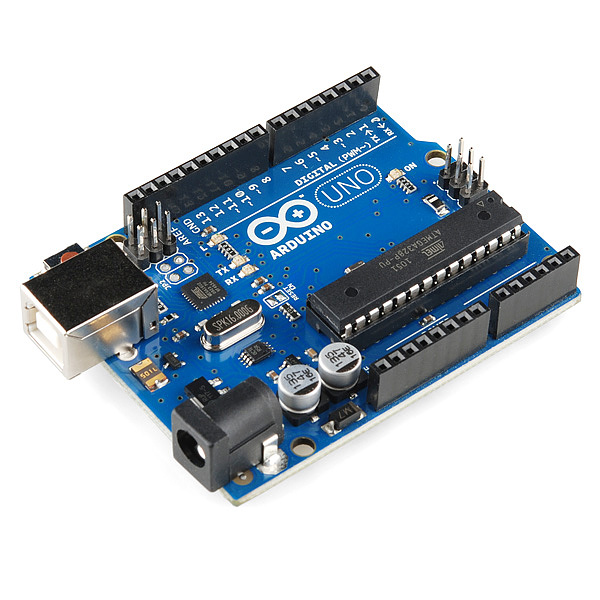
\includegraphics[width=0.6\textwidth]{Chapter2/arduino}
  \caption{Modelo UNO de Arduino.}
\label{fig:arduino}
\end{figure}

Sus principales características son: su facilidad de uso, bajo coste,
multiplataforma, \textit{software} y \textit{hardware} libre y extensible. Todo
esto a propiciado que un gran abanico de usuarios use esta plataforma, desde
estudiantes y profesores hasta artistas y \textit{makers} \cite{arduino-intro}.

Arduino es el estándar \textit{de facto} en los microcontroladores abiertos, no
requiere conocimientos avanzados para realizar pequeños y medianos proyectos y
tiene una gran comunidad que aporta mucha documentación.


\subsubsection{Adafruit Motorshield}
\label{subs:adafruit motor shield}

%TODO: añadir I2C y DC LED a los acrónimos

Diseñado por Adafruit, el MotorShield, figura~\ref{fig:motor-shield},  sirve
para ampliar las prestaciones de las placas Arduino. Esta placa proporciona un
driver MOSFET TB6612 con 1.2A por canal y un driver PWM embebido para controlar
los motores y sus velocidades mediante el protocolo I$^2$C. Mediante esta placa
es posible controlar dos servos de 5V, 4 motores DC (unipolares o bipolares) y
dos motores paso a paso. Añade, además, medidas de seguirdad para evitar problemas,
como bloques termoresistentes o autoapagado por temperatura \cite{motorshield}.

\begin{figure}[htp]
  \centering
    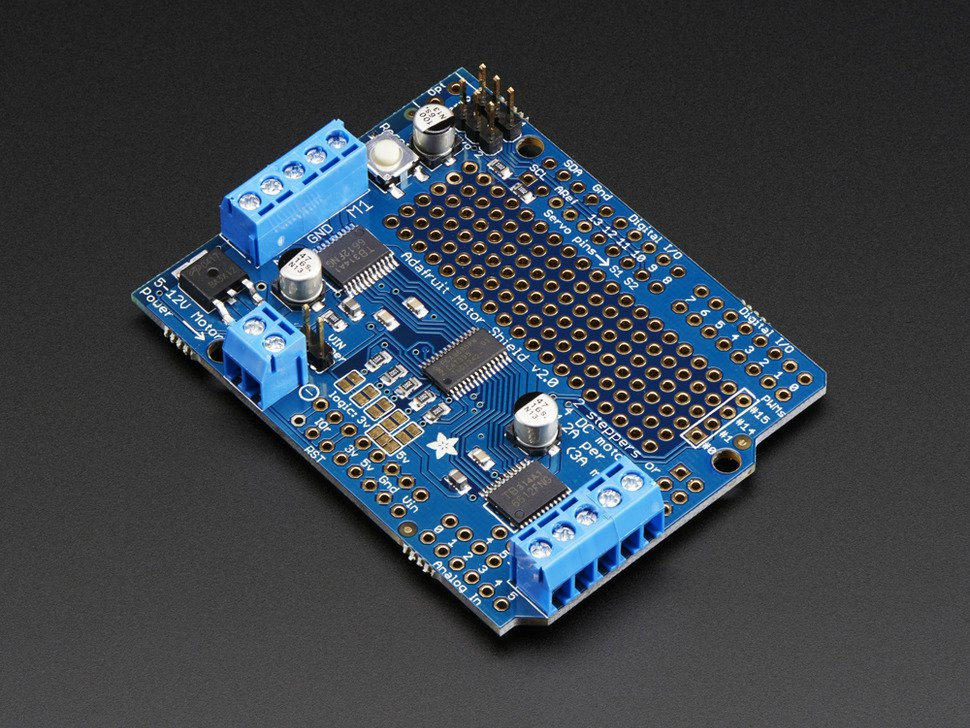
\includegraphics[width=0.7\textwidth]{Chapter2/motor-shield}
  \caption{Vista de la parte superior del MotorShield para Arduino.}
\label{fig:motor-shield}
\end{figure}

\subsubsection{Prusa i3}
\label{subs:prusa-i3}

La impresora Prusa i3 es el útlimo modelo desarrollado por Prusajr. Se caracteriza
por ser un modelo muy popular y en el que mucha gente a basado sus propios diseños
debido a su diseño está licenciado mediante GPL \cite{prusa1}. Otra característica
es que las partes autoreplicables de la impresora están diseñadas de forma
paramétrica, pudiendo adaptar estas piezas a las necesidades de cada persona
\cite{prusa2}.

\begin{figure}[htp]
  \centering
    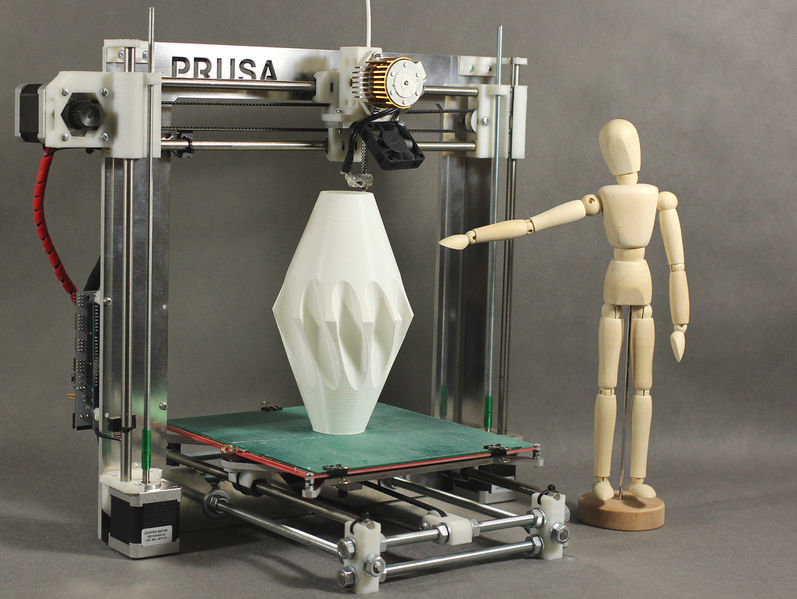
\includegraphics[width=0.8\textwidth]{Chapter2/prusai3}
  \caption{Impresora 3D Prusa i3 con una pieza impresa junto a un muñeco arti-
culado.}
\label{fig:prusai3}
\end{figure}

Debido a la gran cantidad de gente que aporta soluciones y ayuda ha hecho de este
modelo sea la impresora con la que se inicia la gran mayoría de personas. Fue
también el modelo propuesto y que se construyó en el Taller RepRap UA
\cite{TallerRepRap} y a la que se ha tenido acceso durante el desarrollo de
este trabajo.

\subsubsection{Myo}
\label{subs:myo}

%NOTE añadir que el EMG va a 200Mz y el IMU a 50Hz

%TODO añadir IMU unidad de medición inercial, inertial measurement unit
Este dispositivo, creado por Thalmic Labs, es capaz de detectar la actividad
eléctrica ejercida por los músculos mediante el uso de 8 sensores EMG de grado
médico. Además cuenta con un IMU de 9 ejes que contiene un giroscopio de 3
ejes, un accelerómetro de 3 ejes y un magnetómetro de 3 ejes \cite{myo-specs}.


\begin{figure}[htp]
  \centering
    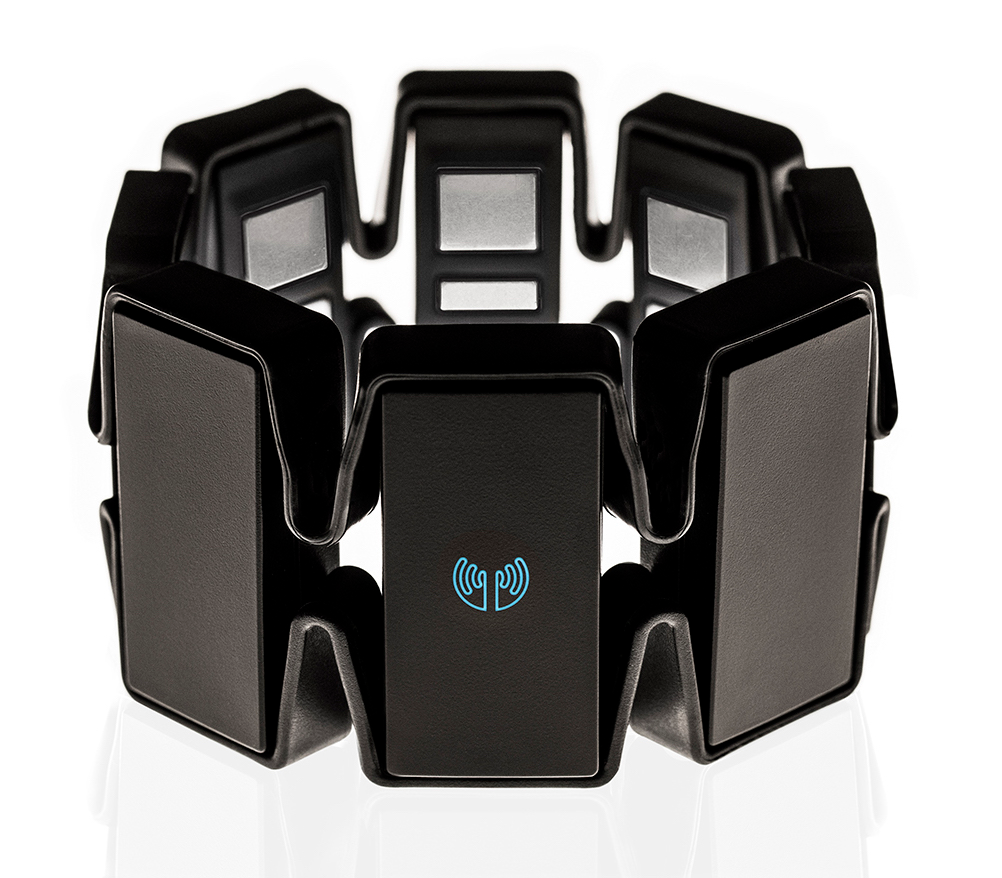
\includegraphics[width=0.5\textwidth]{Chapter2/myo}
  \caption{Vista de frente de la Myo Armband}
\label{fig:myo}
\end{figure}

Gracias a estos sensores, es posible analizar tanto datos EMG, con un rango de
-128 a 128 en unidades de activación. Por otro lado, mediante el IMU se podrán
obtener datos acerca de la orientación y el movimiento del brazo en el que esté
situada la Myo \cite{abduo2015myo}.

A pesar de ser de no ser un proyecto libre, es un prodcuto que ofrece 8 sensores
EMG, se recarga mediante un cable micro USB (el usado por la mayoría de teléfonos
móviles), y no es necesario ningún tipo de complemento adicional, simplemente
se coloca en el brazo del usuario y ya puede usarse puesto que la comunicación
se realiza mediante~\textit{bluetooth}. Por estas facilidades y el número de
sensores de los que dispone, se ha elegido como dispositivo para obtener las
señales EMG.





%%%%%%%%%%%%%%%%%%%%%%%%%%%%%%%%%%%%%%%
%
%
%			PRÓTESIS Y ELECTRÓNICA
%
%
%%%%%%%%%%%%%%%%%%%%%%%%%%%%%%%%%%%%%%%


\section{Prótesis y electrónica}
\label{sec:prótesis-electrónica}
Este apartado resume cómo se ha elaborado el entorno de pruebas con el fin de probar el \textit{software} desarrollado en un entorno real. Se ha utilizado una impresora 3D \ref{subs:prusa-i3} para crear la prótesis Dextrus \ref{sub:bebionic}. Mientras que el control de los motores de la prótesis se ha realizado mediante Arduino \ref{subs:arduino} y una controladora de motores adheriddo a este \ref{subs:adafruit motor shield}.


\begin{figure}[htp]
  \centering
    \includegraphics[width=1\textwidth]{Chapter2/dorsal}
  \caption{Vista del dorsal de la prótesis terminada}
\label{fig:dorsal}
\end{figure}


\begin{figure}[htp]
  \centering
    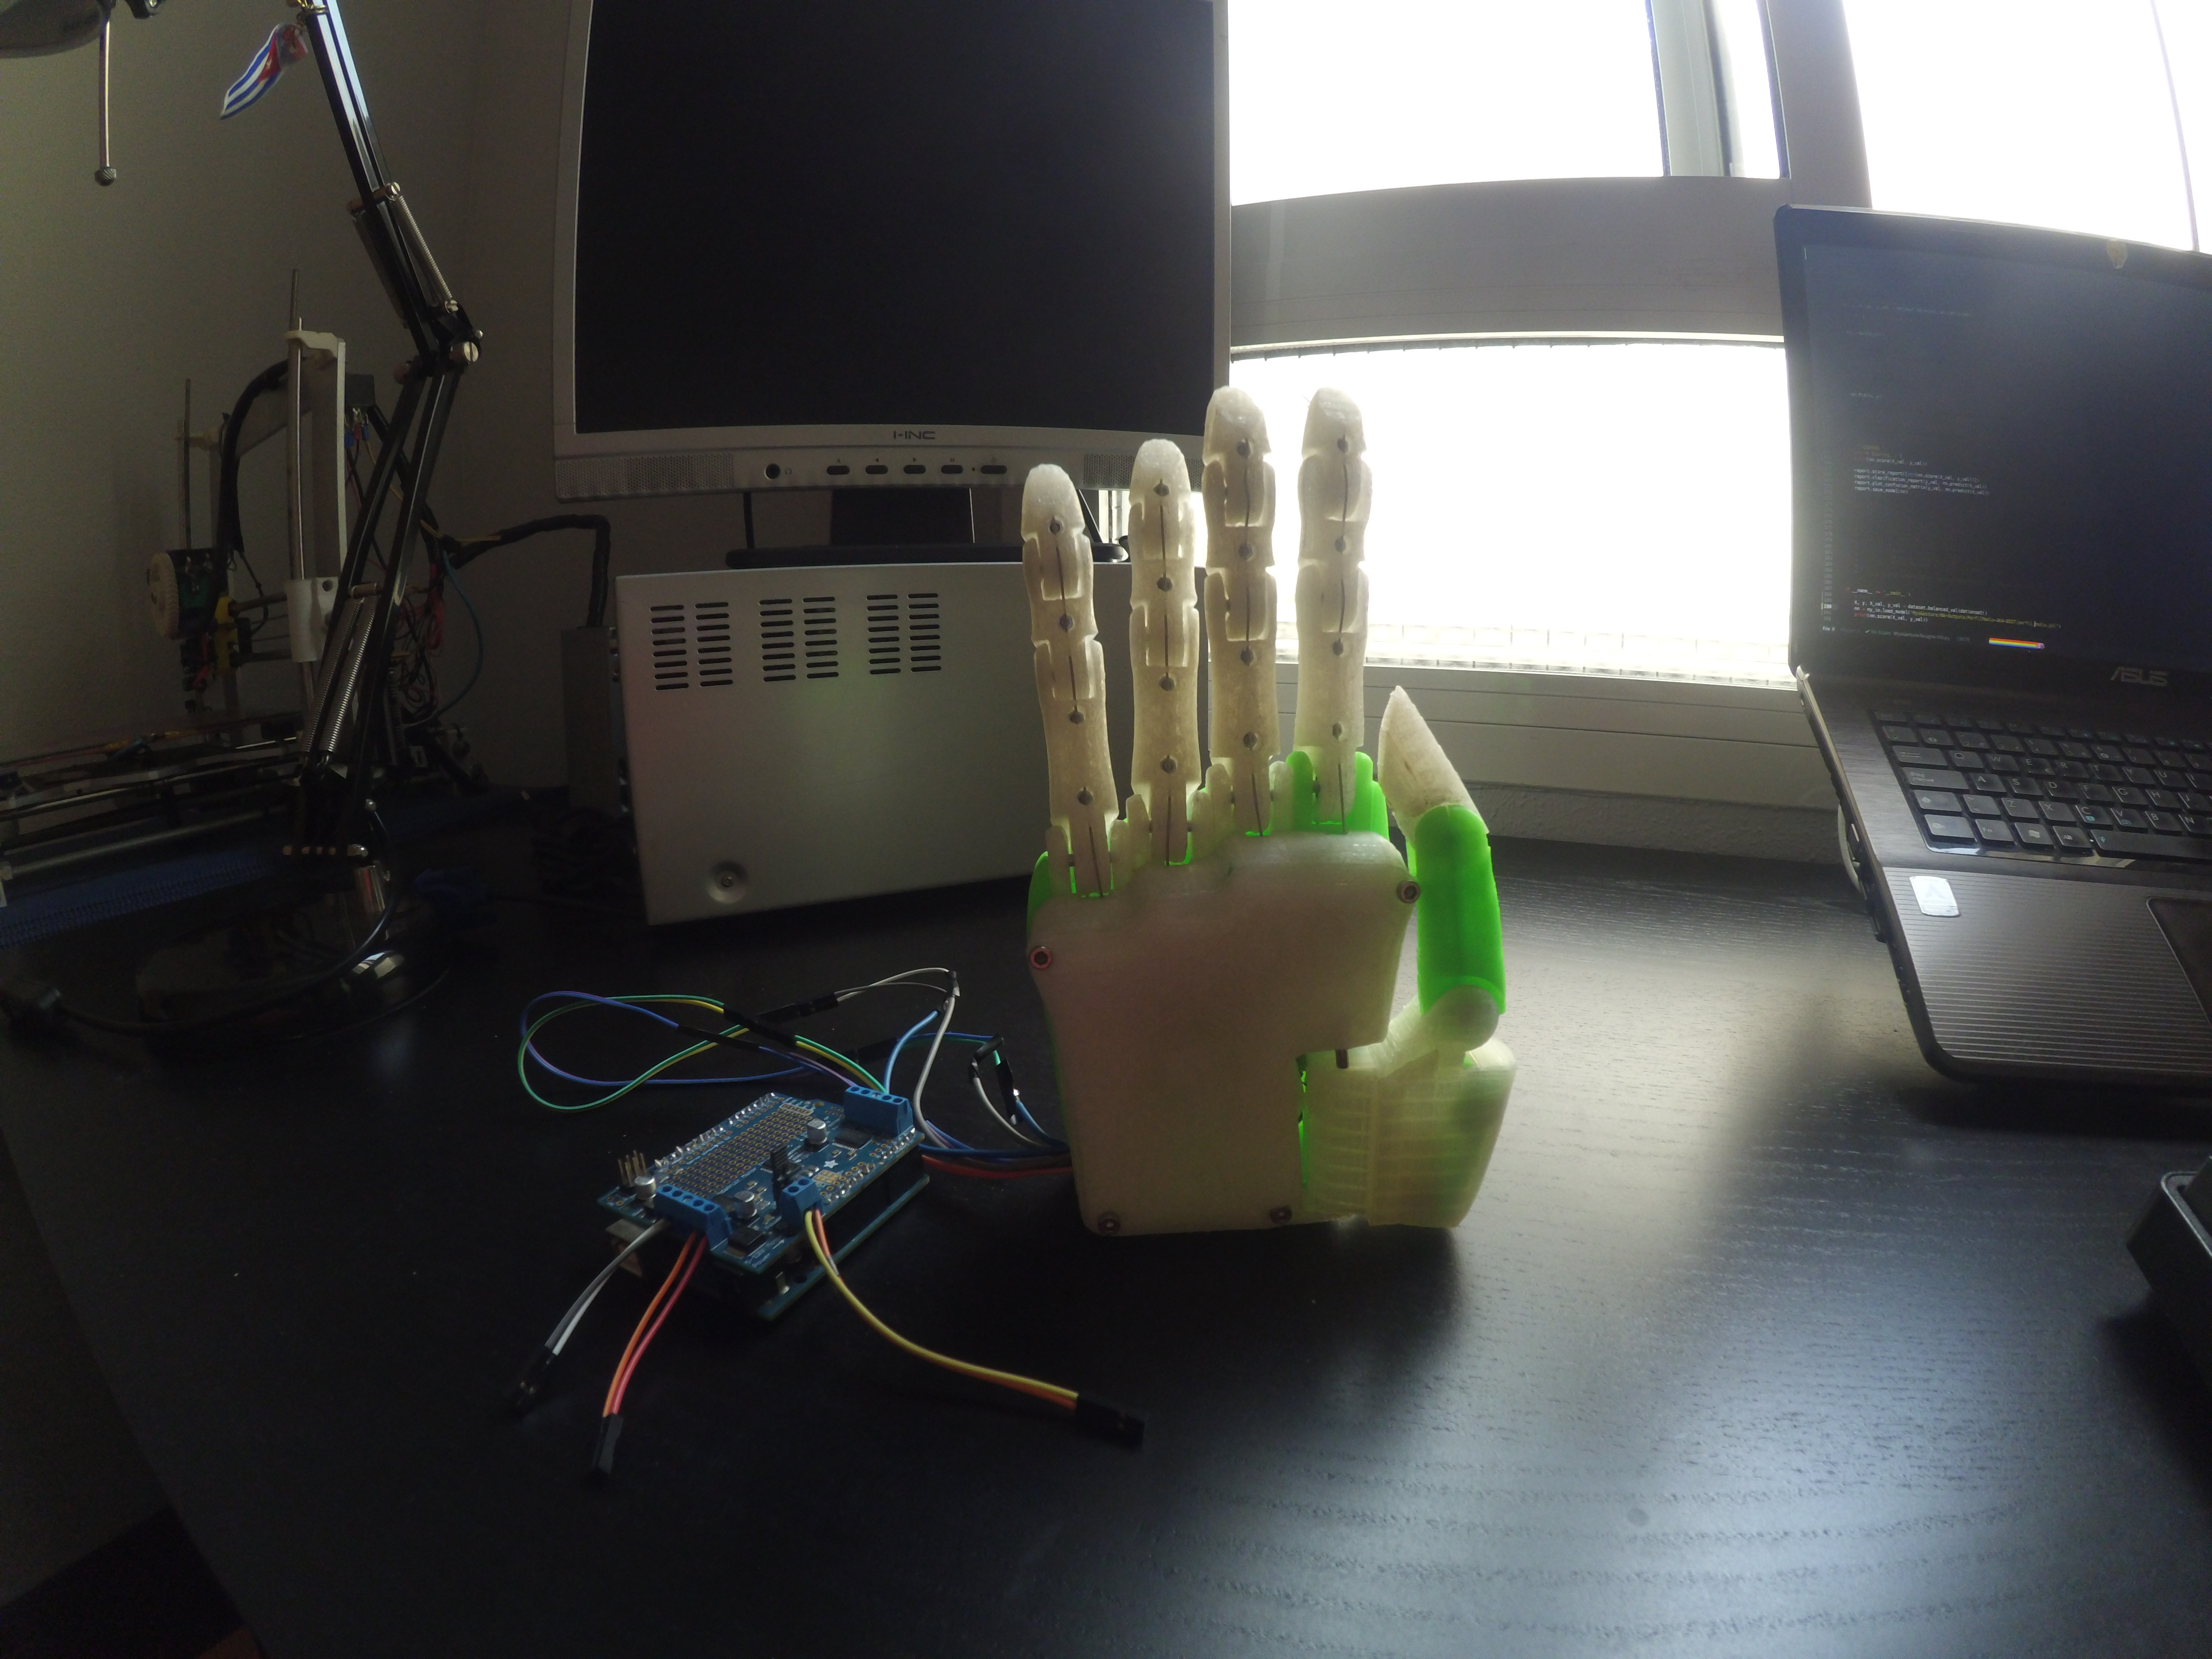
\includegraphics[width=1\textwidth]{Chapter2/palma}
  \caption{Vista del palmar de la prótesis terminada}
\label{fig:palmar}
\end{figure}


\subsection{Desarrollo de la prótesis}

En el anexo \ref{presupuestoProyecto} se especifica los materiales utilizados tanto para la creación de la prótesis como la parte de la electrónica que la controlará.


Los modelos 3D de la prótesis Dextrus \ref{fig:dorsal} \ref{fig:palmar} pueden descargarse en \cite{openbionics-downloads} y las instrucciones del montaje en
\cite{dextrus-instructions}. El mayor problema ha sido encontrar ciertos materiales, en concreto: tornillería de
métrica dos o inferior (tienda de modelismo especializado), los cables que emulan los tendones (hilos métalicos de
pesca), las virolas para unir los dos extremos de los cables (material de pesca) y clavijas o tarugos de metal, que
son las piezas que se introducen en los rodamientos (este ha sido el componente más difícil de encontrar ya que
el modelo de la prótesis requiere longitudes de este componente muy determinadas -se pueden consultar en el anexo
\ref{presupuestoProyecto} -, para conseguirlo se ha tenido que cortar y limar destornilladores de 3mm de anchura a mano).







\subsection{Componentes electrónicos}

La electrónica consiste básicamente en el controlador de motores, que controla el movimiento de los motores de la prótesis, y el Arduino, que se encarga de cuándo deben moverse los motores. Para poder alimentar tanto los
componentes electrónicos como los motores que están dentro de la prótesis, se ha utilizado para el entorno de pruebas una fuente de alimentación de PC (fuera de este entorno la fuente sería sustituida por una batería
recargable, pero esto queda fuera del trabajo y se propone como futuras mejoras).
%TODO añadir batería de a trabajo futuro.

La alimentación a todos los componentes se realiza mediante el controlador de motores, que recibe una tensión de 12V desde la fuente. Para utilizar los cables de esa intensidad \cite{power-pc} de deben seguir los siguientes pasos \textbf{siempre con la fuente desconectada de la red eléctrica}:

\begin{itemize}
\item Crear un puente entre el pin PS\_ON y cualquiera de los cables de toma de tierra (Ver figura \ref{fig:atx-colors} para comprobar los colores).

\item Sacar los cables de 12V de tensión (color amarillo). Se puede usar regletas y cables macho-hembra para facilitar el proceso de conexión y desconexión como se muestra en la figura \ref{fig:mi-fuente}.

\end{itemize}

\begin{figure}[htp]
  \centering
    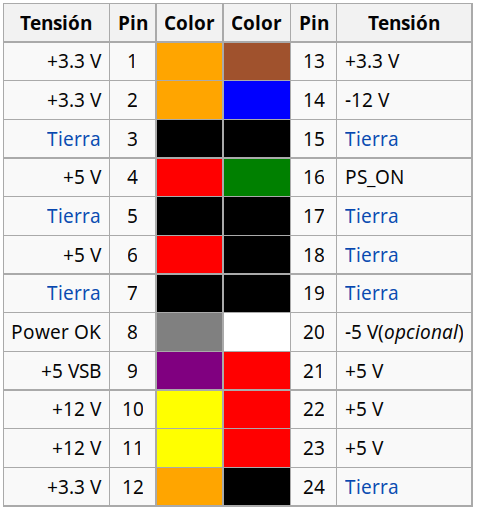
\includegraphics[width=0.6\textwidth]{Chapter2/atx-colors}
  \caption{Información sobre los pines de una fuente de alimentación ATX. Imagen extraida de wikipedia.org}
\label{fig:atx-colors}
\end{figure}



\newpage
\subsection{Entorno de pruebas}

En las figuras \ref{fig:mi-fuente} y \ref{fig:mi-prótesis} se puede observar los componentes que se utilizarán para realizar las pruebas reales con el modelo de clasificación desarrollado a lo largo del proyecto.

\begin{figure}[htp]
  \centering
    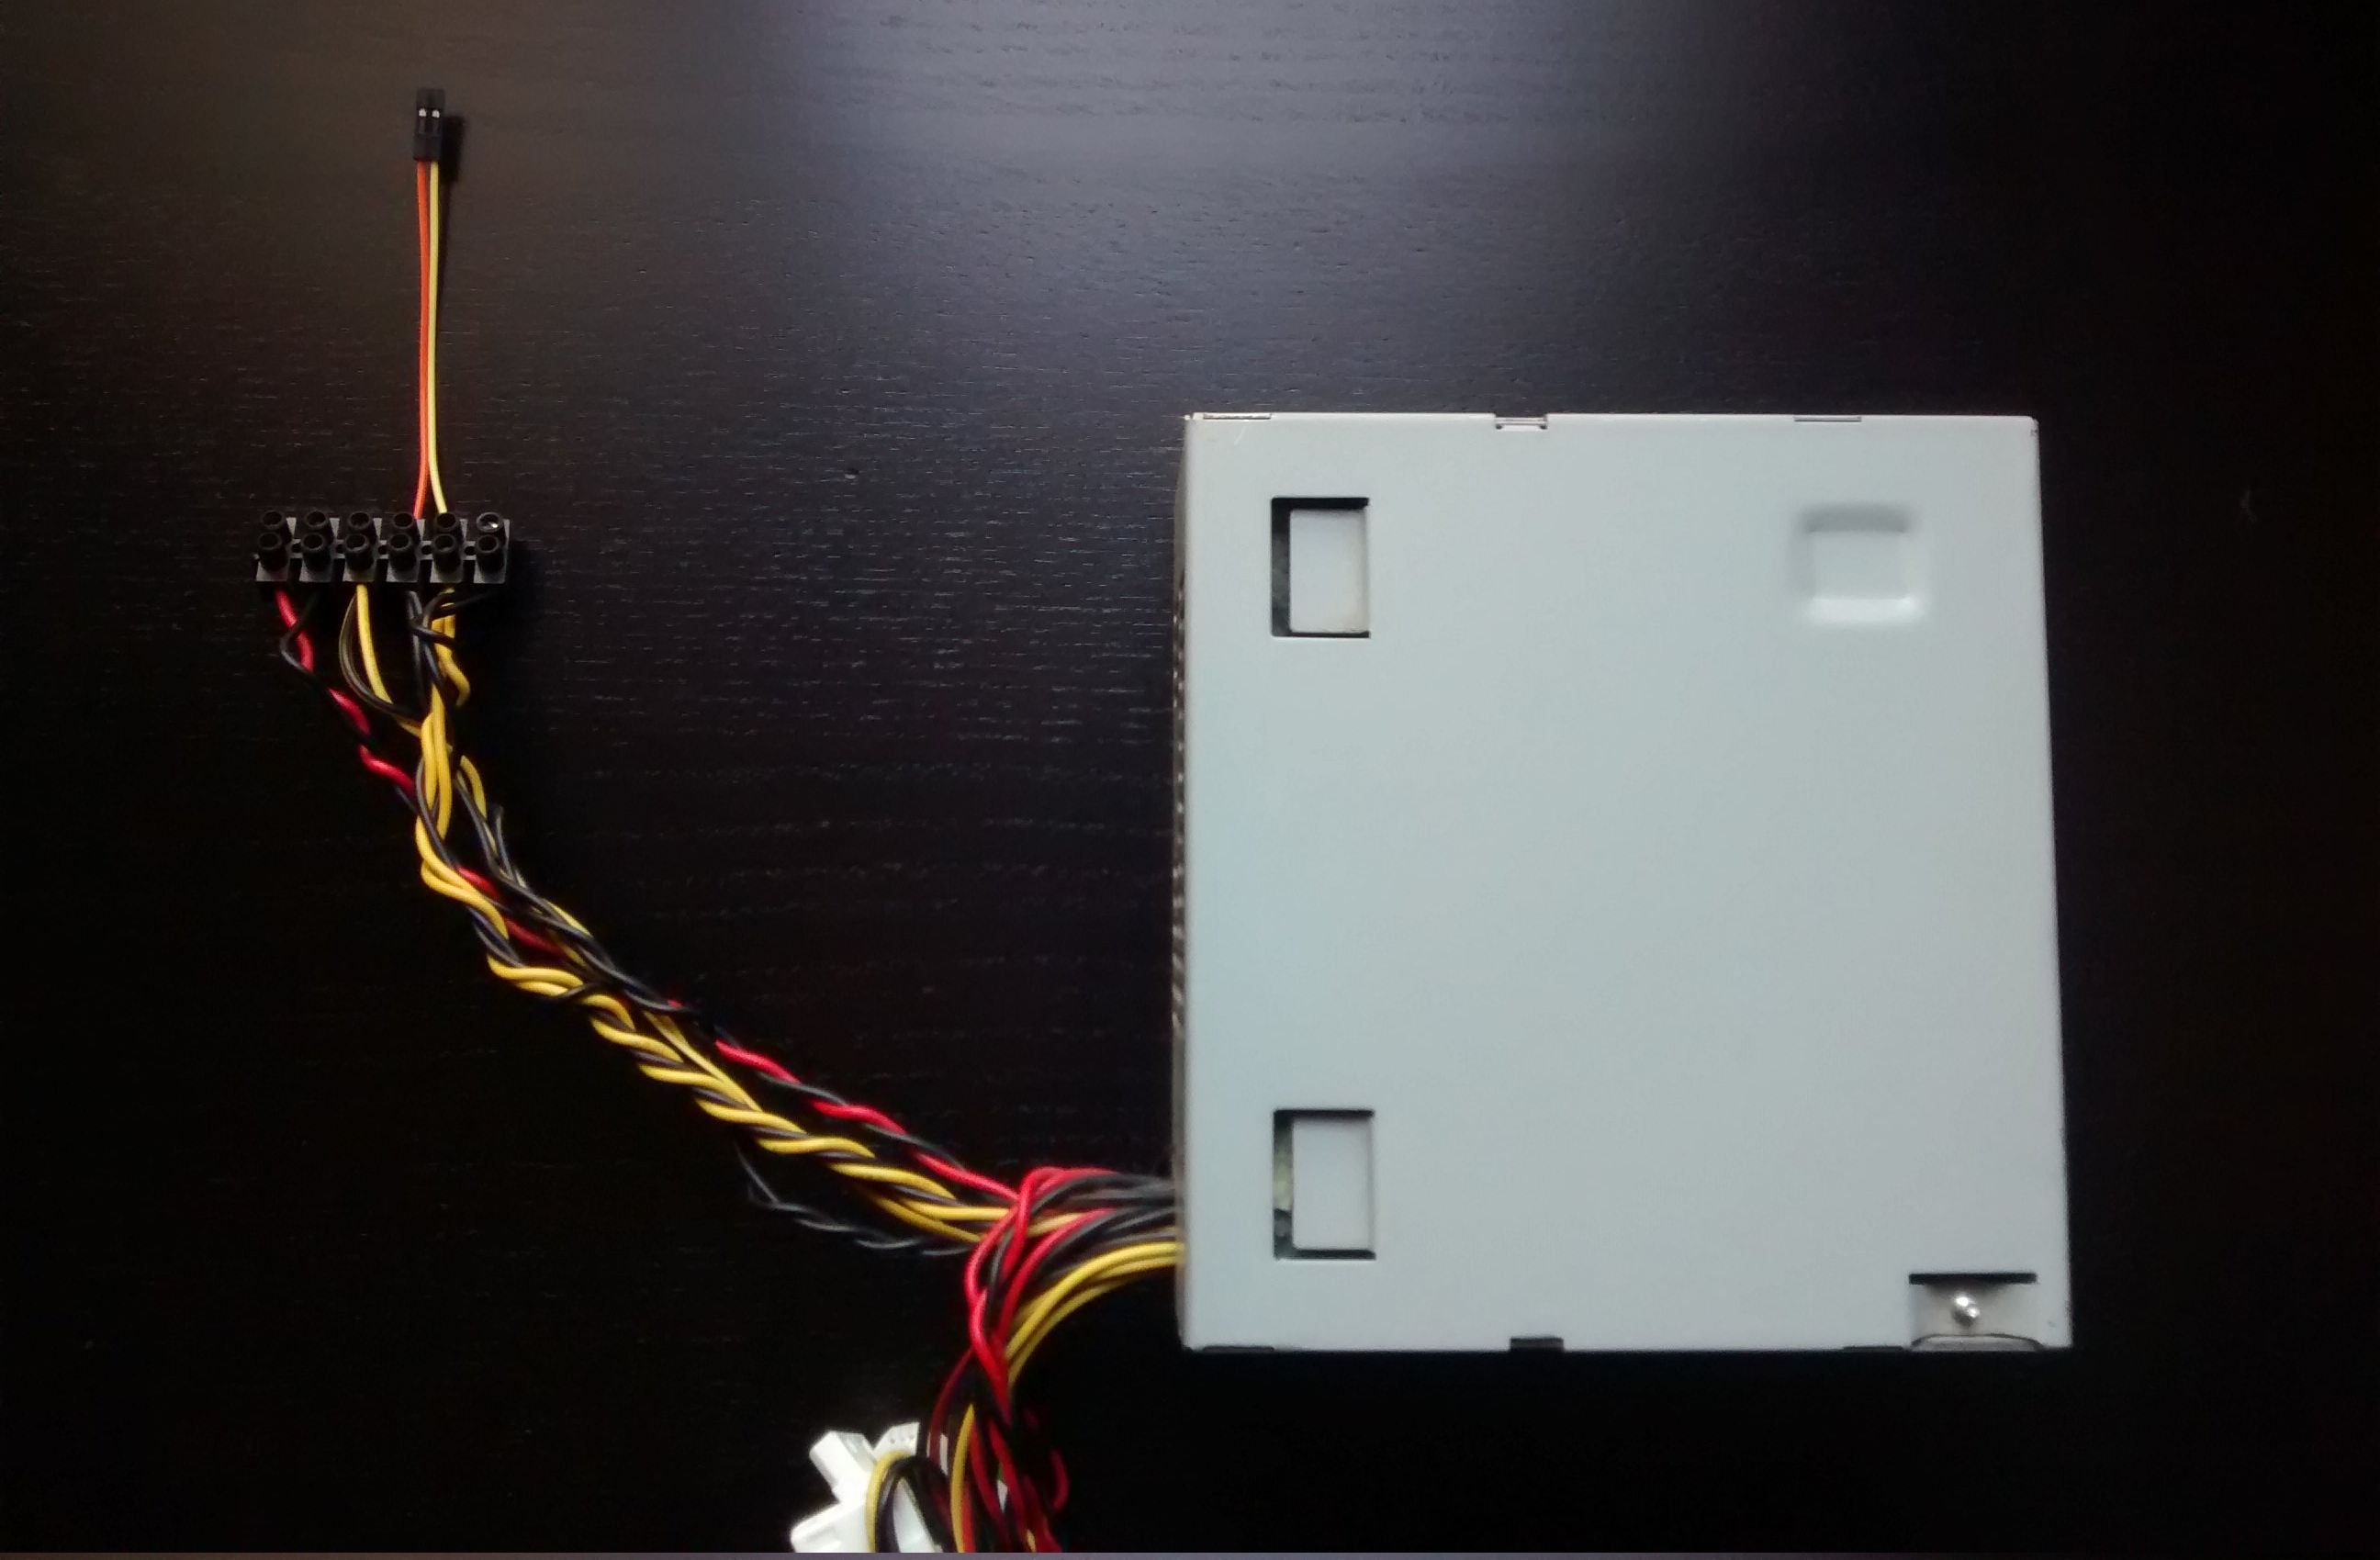
\includegraphics[width=0.85\textwidth]{Chapter2/mi-fuente}
  \caption{Fuente de alimentación preparada para utilizar 12V.}
\label{fig:mi-fuente}
\end{figure}

\begin{figure}[htp]
  \centering
    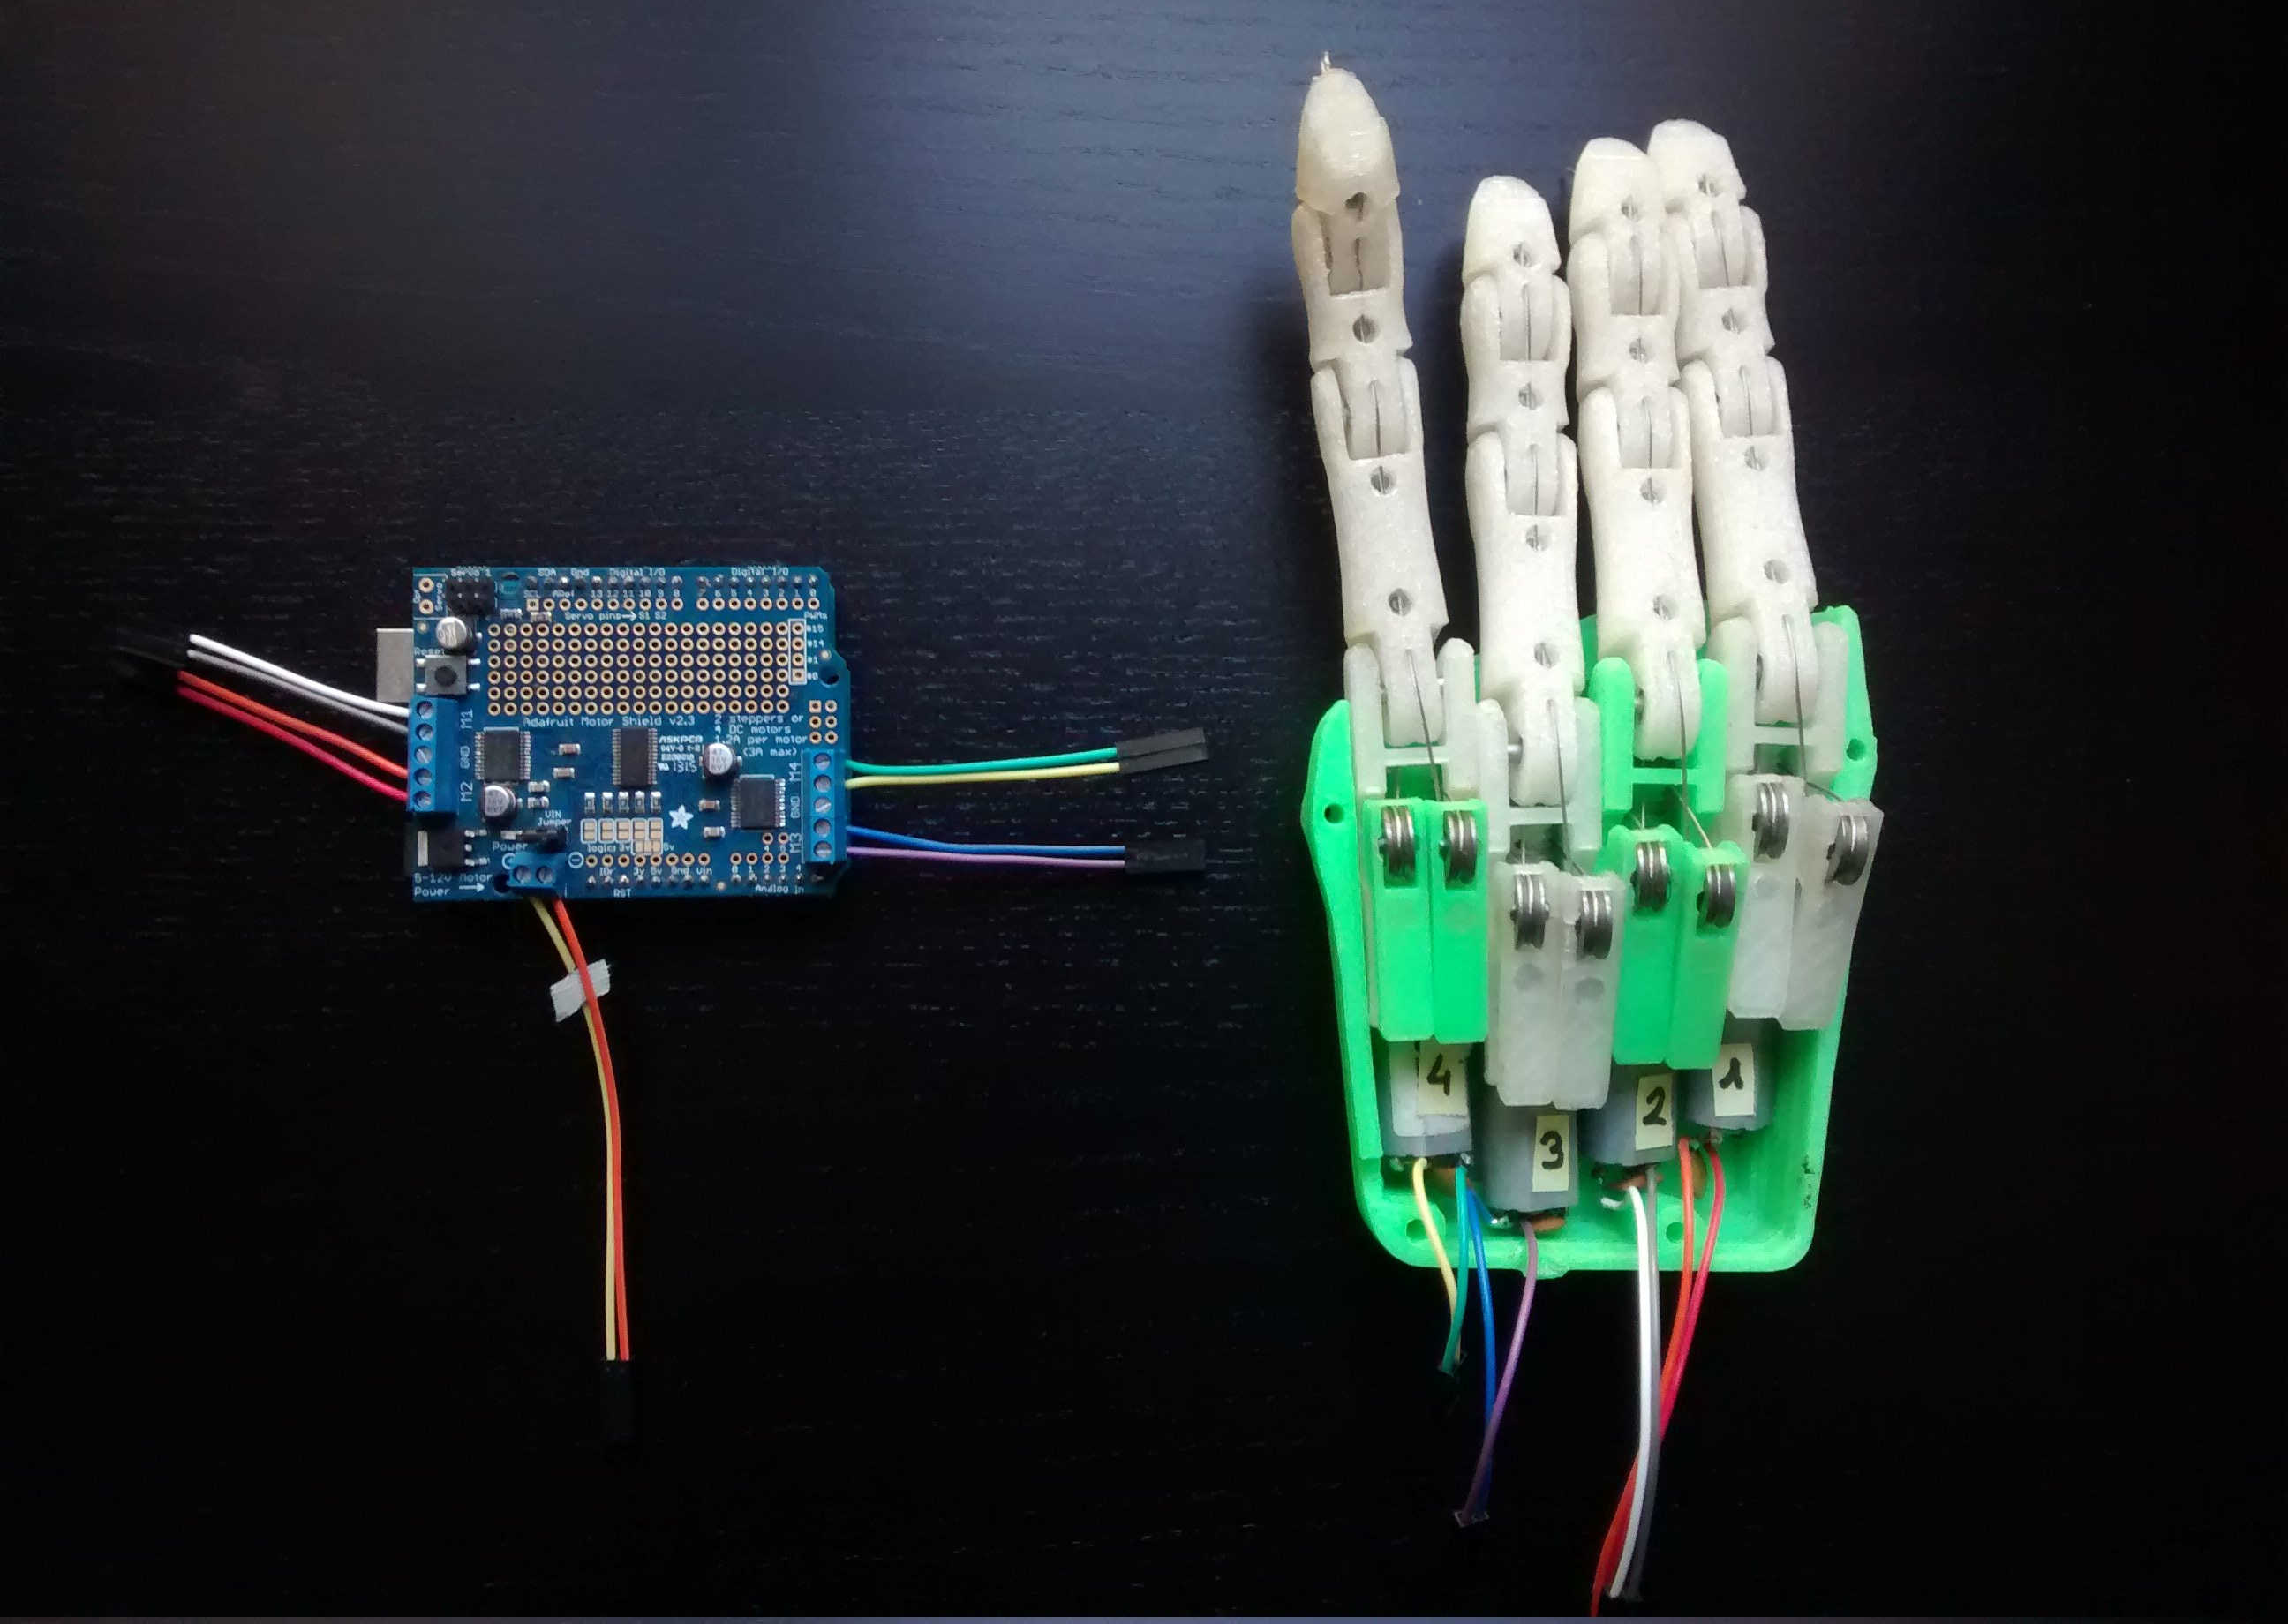
\includegraphics[width=0.85\textwidth]{Chapter2/mi-protesis}
  \caption{Arduino con el controlador de motores acoplado junto con la prótesis y sus componentes al descubierto.}
\label{fig:mi-prótesis}
\end{figure}

\chapter{Aprendizaje automático y \textit{deep learning}}
\label{Chapter3}

\chapquote{
En este capítulo se introducen de forma resumida nociones teóricas
sobre aprendizaje automático y \textit{deep learning}. En el apartado
\ref{sec:introducción-aprendizaje} se define formalmente qué es el aprendizaje automático y se resume
qué tipos de aprendizaje hay. En el apartado \ref{sec:redes-neuronales} se explica qué son
las redes neuronales artificiales y el modelo de red utilizado en este
proyecto.}


\section{Introducción}
\label{sec:introducción-aprendizaje}

Mediante el uso de algoritmos de aprendizaje automático se pueden crear modelos que, a partir de una colección de datos, sean capaces de tomar decisiones. Formalmente, \cite{mitchell1997machine} define el aprendizaje automático como
``Se dice que un programa aprende de la experiencia E respecto a un tipo de trabajo T con una medida de rendimiento R, cuando el rendimiento de una tarea T medido por R mejora con la experiencia E''. El enfoque de este trabajo es práctico, por lo que no se entrará en detalles filosóficos como qué es la consciencia o biológicos sobre cómo se han formalizado las redes neuronales a partir del concepto de neuronas.

Así pues, podemos definir principalmente dos tipos de tareas que corresponden a dos tipos de aprendizaje:

\begin{itemize}
  \item Aprendizaje supervisado: las muestras contienen atributos que se
  quieren predecir. Dependiendo del resultado que se busque, se distingue
  a su vez entre:

    \begin{itemize}
%      \item Clasificación: cuando el resultado es ``discreto'', es decir, se busca
%      que una muestra pertenezca a una clase a partir de un conjunto de muestras
%      que haya sido clasificado previamente.

      \item Clasificación: el programa determina qué datos de entrada (muestras) pertenecen a qué categoría. Por
      ejemplo, dado la longitud de un pétalo y su color(muestras), se puede determinar a qué especie pertenece
      (categoría).

      \item Regresión: la predicción de este tipo de tareas es una variable contínua, es decir, dado un conjunto
      de muestras, predice un valor real. Por ejemplo, estimar el valor de alquiler de una zona residencial dado un
      número de habitantes y sus ingresos económicos.

    \end{itemize}

    \item Aprendizaje no supervisado: donde ninguna de las muestras está clasificada y el objetivo es inferir
   similitudes patrones con el fin de agruparlas en distintos conjuntos.

\end{itemize}

El problema que se plantea en este trabajo, es un problema de clasificación,
puesto que el resultado que se espera es un número real comprendido entre 0 y 5 que representará la longitud que la
prótesis debe procesar para estirar el dedo. Las muestras serán los 8 valores de cada sensor EMG que posee la Myo.


\section{Redes neuronales artificiales}
\label{sec:redes-neuronales}
Para resolver el problema de clasificar señales EMG en etiquetas de longitudes, se ha implementado una red neuronal prealimentada (\textit{feedforward neural network}) o perceptrón multicapa (MLP por sus siglas en inglés, \textit{Multilayer perceptron}). Este tipo de modelo, pertenecen al \textit{deep learning}, una rama del aprendizaje automático \cite{Goodfellow-et-al-2016-Book}.

%TODO añadir acrónimo MLP

El objetivo de un MLP es intentar definir una función \textit{f}, formalmente:
%y=f(x;\theta)
\begin{equation}
	y=f(x;\theta)
\end{equation}

donde \textit{y} es la etiqueta resultante, \textit{x} los datos de entrada y $\theta$ el valor de los parámetros \cite{Goodfellow-et-al-2016-Book}. Este tipo de redes ha dado lugar a la resolución de problemas de reconocimiento de voz, reconocimiento de objetos, procesamiento de señales entre otros \cite{DBLP:journals/corr/abs-1206-5538}.

Estructuralmente, como podemos ver en la figura \ref{fig:red-neuronal} se componen de distintos elementos inspirados
por la neurociencia \cite{riesenhuber1999hierarchical} (aunque su funcionamiento es matemático y el objetivo es obtener funciones, no recrear neuronas o un cerebro biológico). Los elementos principales son:


\begin{itemize}
	\item Capa de entrada: las muestras de las que se quiere aprender son introducidas en esta primera capa.

	\item Capa oculta: recibe como entrada las salidas de la capa de entrada u otras capas ocultas. Estas capas
	contienen un número determinado de neuronas o unidades que contienen cada una de ellas su propio valor de
	activación.

	\item Capa de salida: dependiendo del tipo de problema la capa de salida implementa determinada función para
	obtener los resultados esperados. Por ejemplo, un problema de clasificación multiclase implementará una
	función \textit{softmax} (obteniendo una salida), mientras que para clasificaciones multietiqueta se usaría
	una función \textit{sigmoid} (obteniendo más de una salida).
\end{itemize}


\begin{figure}[htp]
    \centering
    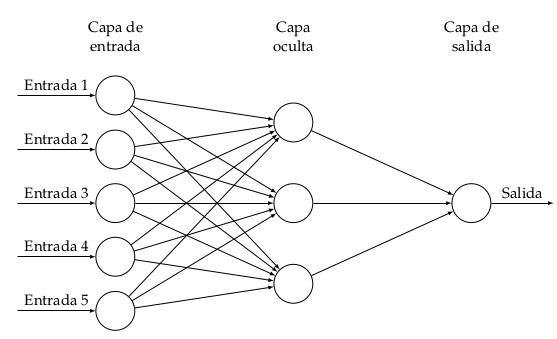
\includegraphics[width=1\textwidth]{Chapter3/neural-net}
\caption{Ejemplo de red neuronal prealimentada de cinco entradas y una salida.}
\label{fig:red-neuronal}
\end{figure}



Puesto que el objetivo del trabajo es poner en funcionamiento una modelo de clasificación multiclase no se entrará en más detalles del funcionamiento interno de este tipo de redes. No obstante, en los siguientes subapartados se explicarán algunas técnicas utilizadas durante el desarrollo del perceptrión multicapa en capítulo \ref{Chapter4}

\newpage


\subsection{Dropout}
\label{subs:dropout}

Existe una situación en la que durante el entrenamiento de un modelo podemos obtener altas tasas de acierto mientras que al usar el conjunto de validación o datos reales -es decir, cuando el software está en producción- tiene un rendimiento muy bajo, esto es debido al sobreentrenamiento (\textit{overfitting} en inglés).

Para contrarrestar este efecto se utiliza de forma extendidada técnicas como los términos de regularización L1 y L2,
que básicamente son funciones que penalizan ciertas configuraciones de parámetros \citep{xu2010l1}. No obstante,
para las redes neuronales existe otra técnica que además de ofrecer una solución al sobreentrenamiento permite
acortar los tiempos de entrenamiento. Esta técnica se denomina \textit{dropout} \citep{JMLR:v15:srivastava14a}, y consiste en, de forma aleatoria, desconectar unidades (o neuronas) de la red como se muestra en la figura \ref{fig:dropout}.

\begin{figure}[htp]
    \centering
    \begin{subfigure}[b]{0.3\textwidth}
        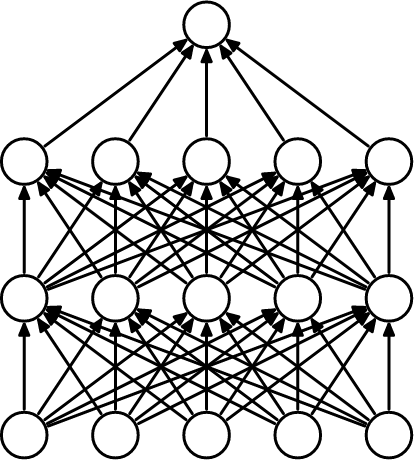
\includegraphics[width=\textwidth]{Chapter3/dropout-before}
        \caption{Red neuronal original.}
        \label{fig:dropout-before}
    \end{subfigure}
    \qquad
     %add desired spacing between images, e. g. ~, \quad, \qquad, \hfill etc.
      %(or a blank line to force the subfigure onto a new line)
    \begin{subfigure}[b]{0.3\textwidth}
        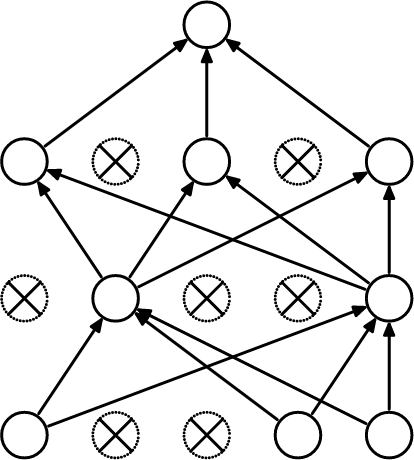
\includegraphics[width=\textwidth]{Chapter3/dropout-after}
        \caption{Despúes de aplicar \textit{dropout}.}
        \label{fig:dropout-after}
    \end{subfigure}
     %add desired spacing between images, e. g. ~, \quad, \qquad, \hfill etc.
    %(or a blank line to force the subfigure onto a new line)
    \caption{Comparación tras aplicar \textit{dropout} a una red neuronal. Las unidades marcadas con una X son las que han sido apartadas aleatoriamente en esta iteración. (Figura extraída de \citep{JMLR:v15:srivastava14a})}\label{fig:dropout}
\end{figure}



\newpage



\subsection{Inicialización Glorot}

El algoritmo Glorot (también llamado Xavier \cite{glorot2010understanding}) determina el valor de todos los pesos
iniciales de la red basándose en el número de entradas y salidas de las neuronas \cite{glorot-lasagne}. Existen distintas implementaciones para esta función, sobretodo dependiendo el programa o \textit{framework} que se utilice, aunque los autores \cite{glorot2010understanding} originalmente la definen como :

\begin{equation}
Var(W)=\frac{2}{n_{in}+n_{out}}
\end{equation}

Esta función permite regular la inicialización de los pesos de la red de forma correcta, puesto que un valor de
inicio pequeño se perdería según fuera avanzando en la red; mientras que, uno grande, iría incrementándose hasta ser
demasiado grande como para ser útil.


\subsection{Funciones no lineales}

El propósito de las funciones de activación es introducir nolinearidad a la red con tal de que las salidas no puedan ser reproducidas mediante una combinación lineal de las entradas.

A continuación se muestra alguna de las funciones utilizadas en el apartado de experimentación [\ref{sec:experimentación}] del capítulo \ref{Chapter4}.


\subsubsection{Rectificador}

Se define la función \textit{rectify} como:

\begin{equation}
f(x) = max(0, x)
\end{equation}

La figura \ref{fig:rectify} representa esta función en una gráfica para los valores de x comprendidos entre -5 y 5.

\begin{figure}[ht]
  \centering
    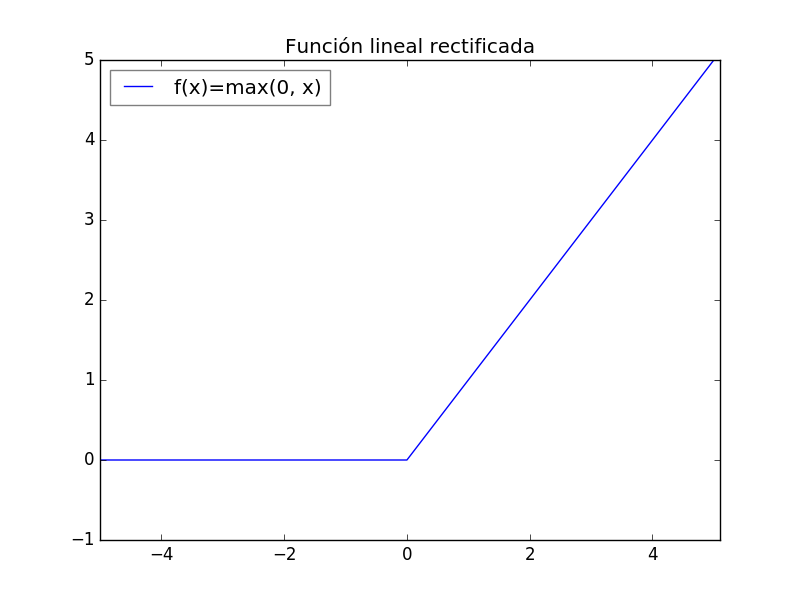
\includegraphics[width=1\textwidth]{Chapter3/rectify}
  \caption{Valores que toma la función \textit{rectify}}
\label{fig:rectify}
\end{figure}


\subsubsection{Tangente hiperbólica}

La functión \textit{tanh} se define formalmente en \ref{tanh} y su representación en un gráfico en \ref{fig:tanh}

\begin{equation}
f(x) = tanh(x)
\label{tanh}
\end{equation}

\begin{figure}[ht]
  \centering
    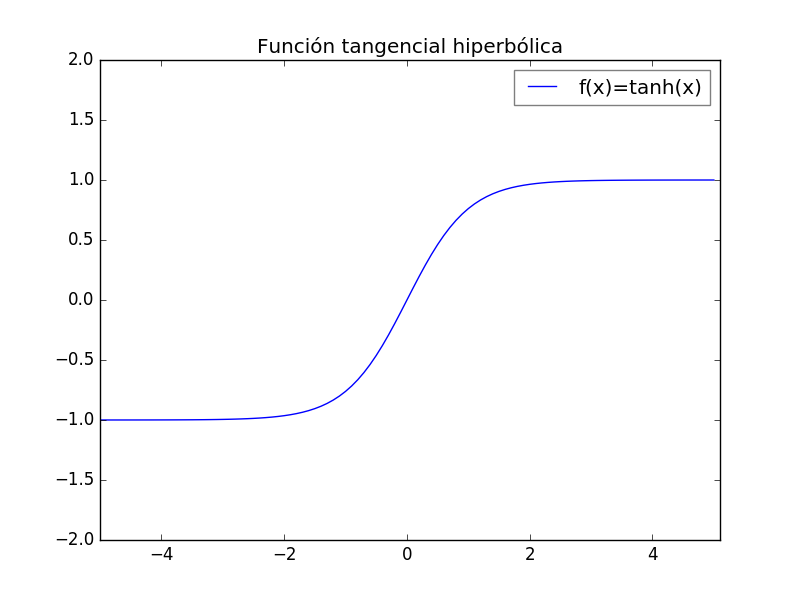
\includegraphics[width=1\textwidth]{Chapter3/tanh}
  \caption{Valores que toma la función \textit{tanh}}
\label{fig:tanh}
\end{figure}


\subsubsection{Sigmoidea}

La última función probada como función de activación en la red funcional es la función \textit{sigmoid}:

\begin{equation}
f(x)=\frac{1}{1+{e}^{-x}}
\end{equation}

Y para los valores de x entre -5 y 5, la función tiene el aspecto que se muestra en la figura \ref{fig:sigmoid}.


\begin{figure}[ht]
  \centering
    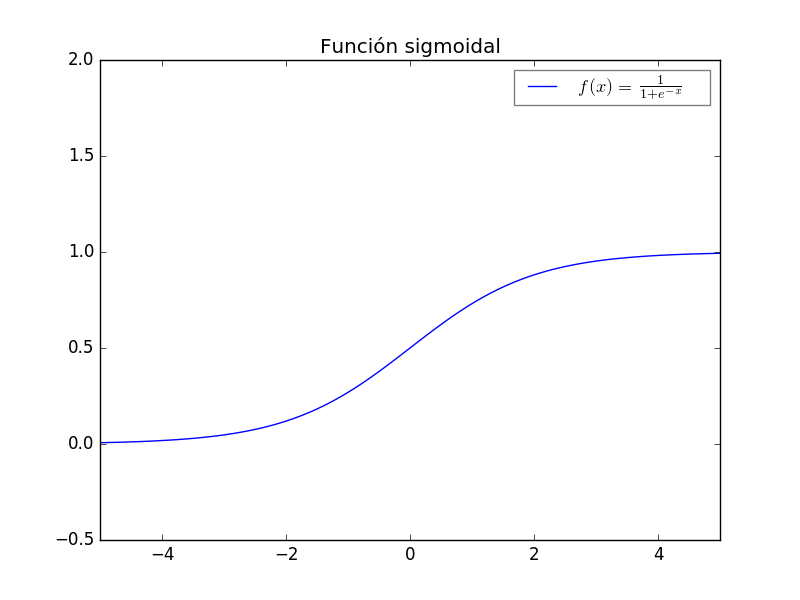
\includegraphics[width=1\textwidth]{Chapter3/sigmoid}
  \caption{Valores que toma la función \textit{sigmoid}}
\label{fig:sigmoid}
\end{figure}

% Chapter Template

\chapter{Obtención y clasificación de señales EMG} % Main chapter title

\label{Chapter4} % Change X to a consecutive number; for referencing this chapter elsewhere, use \ref{ChapterX}

\chapquote{En este capítulo se describe la implementación de la idea propuesta en el capítulo \ref{Chapter1}
utilizando las herramientas y tecnologías descritas en el capítulo \ref{Chapter2}.
En el apartado \ref{sec:obtención-señales} se explica el código desarrollado para captar y guardar las señales EMG y
su etiqueta de longitud correspondiente. En el apartado \ref{sec:clasificación-señales-emg} se explicará el modelo de clasificación implementado. Y por último, en el apartado \ref{sec:experimentación} se describe el proceso que se ha llevado a cabo para optimizar el rendimiento del modelo y se muestran los resultados obtenidos.}






%%%%%%%%%%%%%%%%%%%%%%%%%%%%%%%%%%%%%%%%%%%%%%%%%%%%%%%%%%%%%%%%
%
%
%        OBTENCIÓN DE SEÑALES EMG
%
%
%%%%%%%%%%%%%%%%%%%%%%%%%%%%%%%%%%%%%%%%%%%%%%%%%%%%%%%%%%%%%%%%

\section{Obtención de las señales EMG}
\label{sec:obtención-señales}
Para lograr capturar los datos de la Myo correctamente, se ha desarrollado dos \textit{scripts}
que permiten captar las señales EMG durante el movimiento del dedo (estirar y encoger) y
asociarlas a una etiqueta determinada.

Para captar el movimiento del dedo y poder tratar los datos \textit{a posteriori} se han utilizado
utilizado una \textit{webcam} y un fondo blanco (para poder facilitar el proceso de discernir la
mano del entorno). Una vez colocada la Myo en el brazo del usuario y preparado el entorno,
se puede proceder a iniciar el primer \textit{script}, \textit{data\_recorder.py}, encargado de orquestar
todo el proceso de obtención, etiquetado y grabado de los datos. %TODO: hacer referencia a los listings y hacer un pequeño resumen aqui.

El código \ref{setup} utiliza OpenCV \ref{subs:resultados} para poder mostrar por pantalla las imágenes que toma la
\textit{webcam}, en la figura \ref{fig:obtencion-señal-interfaz} puede verse cómo un usuario interactuaría con el programa. Utiliza además la interfaz de comunicación para la Myo \ref{subs:myo-raw} para abrir la conexión
con ésta.

\begin{figure}
    \centering
    \begin{subfigure}[b]{0.3\textwidth}
        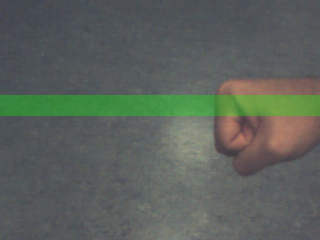
\includegraphics[width=\textwidth]{Chapter4/not-recording}
        \caption{A la espera de entrar en modo grabación.}
        \label{fig:not-recording}
    \end{subfigure}
    ~ %add desired spacing between images, e. g. ~, \quad, \qquad, \hfill etc. 
      %(or a blank line to force the subfigure onto a new line)
    \begin{subfigure}[b]{0.3\textwidth}
        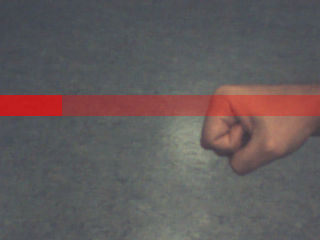
\includegraphics[width=\textwidth]{Chapter4/recording-20}
        \caption{En proceso de grabación, 20\%}
        \label{fig:recording-20}
    \end{subfigure}
    ~ %add desired spacing between images, e. g. ~, \quad, \qquad, \hfill etc. 
    %(or a blank line to force the subfigure onto a new line)
    \begin{subfigure}[b]{0.3\textwidth}
        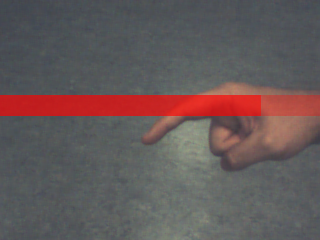
\includegraphics[width=\textwidth]{Chapter4/recording-80}
        \caption{Modo grabación al 80\%}
        \label{fig:recording-80}
    \end{subfigure}
    \caption{Interfaz de usuario para tomar los datos EMG.}\label{fig:obtencion-señal-interfaz}
\end{figure}

\begin{python}[frame=none, numbers=left, label={setup}, caption={Conexión de la \textit{webcam} y la Myo}]
def run(cam_port):
    # Camera set up
    cam = cv2.VideoCapture(cam_port)
    hd.set_up(cam)

    # Myo set up
    m = myo.MyoRaw(sys.argv[1] if len(sys.argv) >= 2
    			    else None)
    m.connect()
    is_disconnected = False

\end{python}



\begin{python}[frame=none, numbers=left,label={data-recorder}, caption={El algoritmo implementado muestra una ventana con la imagen de la \textit{webcam}, cuando el usuario presiona la tecla \textbf{r}(línea 8) se crea un proceso (l. 15) que guarda los
valores que capta la Myo. Se puede diferenciar el ''modo grabación'' cuando la franja cambia de verde \ref{fig:not-recording} a rojo \ref{fig:recording-20} \ref{fig:recording-80} Al pasar un tiempo determinado (l. 19), se procede a recuperar los datos EMG (l.29) así como los de las etiquetas de longitud (l. 30-32). Estos datos son asociados (l.35) y guardados (l.38) }]
def run(cam_port):
...
# Start
while(True):
    # Take a frame form the webcam
    ok, frame = cam.read()
    # Start collecting data when r (recording) is pressed
    if cv2.waitKey(1) & 0xFF == ord('r'):
        # Flag to start the recording's state
        recording = True
        # Set up a thread for recording emg values
        startRecording = time.monotonic()
        # Set up the emg recoerder thread
        emg_queue = Queue()
        p = Process(target=process_run_myo, args=(m, emg_queue, ))
        p.start()
    if recording:
        # Stop recording after hd.RECORD_TIME seconds
        elapsedTime, finished = is_record_finished(startRecording)
        # The guide turns red when recording
        userImg = hd.add_guide(frame.copy(), COLOR_RED)
        # Shows the remaining time until the record ends
        userImgProgress = hd.add_progress(userImg, COLOR_RED,
                                          elapsedTime)
        cv2.imshow('Capture finger lenght', userImgProgress)
        if finished:
            # Save emg values
            p.join()
            emg = emg_queue.get()  # emg is a queue
            fingerList = [queue_length.get()
                             for i in range(0, queue_length.qsize())]
            finger = deque(normalize(fingerList))
            queue_length = Queue()
            # Label each emg value with a finger length [0 - 5]
            dictLabeledData = label_data(emg, finger)
            # Save in a file the data
            num_records += 1
            my_io.save_dict_to(dictLabeledData,
                               name_data_file+str(num_records))
            recording = False
        else:
            p2 = Process(target=process_finger_length,
                         args=(frame, elapsedTime, queue_length, ))
            p2.start()
    # while not recording, show the user-friendly image
    else:
        userImg = hd.add_guide(frame.copy(), (0, 255, 0))
        cv2.imshow('Capture finger lenght', userImg)
cam.release()
cv2.destroyAllWindows()

\end{python}


Por otra parte, el \textit{script hand\_ detection.py} es el encargado de todo lo relativo a las imágenes
captadas por la \textit{webcam}. En el método \ref{finger-length} se aplican distintas técnicas sobre una imagen
RGB para transformarla en una imagen binarizada. Esta imagen es usada en el método \ref{finger-threshold} para
determinar exactamente la longitud del dedo para utilizarla como etiqueta.

\begin{python}[frame=none, numbers=left, label={finger-length},
caption={Este método aplica diversos tratamientos
sobre la imagen para obtener la etiqueta de longitud. Primero se cambia el espectro de color a HSV (línea 3)
\cite{hsv}, se aplica un desenfoque gaussiano (l. 5)\cite{gaussian-blur}. Una vez realizado se aplica a la
imagen un filtro usando un rango de valores (l.7) para obtener la etiqueta de longitud para esa imagen determinada
(l. 11)  }]
def get_finger_strech_and_H_value_from_img(raw_frame):
    # Convert the frame into HSV image
    hsvImg = cv2.cvtColor(raw_frame, cv2.COLOR_BGR2HSV)
    # Apply a blur to clean up the frame
    blurImg = cv2.GaussianBlur(raw_frame, (3, 7), 0)
    # Apply a threshold to try to binarizing the image
    threshImg = cv2.inRange(blurImg, FINGER_MIN, FINGER_MAX)
    # Get the H values for the image
    hValues = mean_h_value_for_img(threshImg)
    # Get the finger lenght
    fingerLen = finger_length(hValues)
    return hValues, fingerLen
\end{python}


\begin{python}[frame=none, numbers=left,label={finger-threshold}, caption={Función que determina en que punto de la empieza el dedo.
Se calcula un límite con el valor de los primeros 40 píxeles que pertenecen al fondo (línea 3), cuando el valor
de la imagen varía significativamente (l. 7) se ha localizado el inicio del dedo (l. 8), y por tanto su longiutd.}]
def finger_length(hValues):
    threshold = sum(hValues[0:40])/40

    for i in range(40, len(hValues)):
        # Find the value that is higher than the threshold
        if hValues[i] < threshold:
            return IMG_WIDTH - i

    # In case of error return -1
    return -1
\end{python}

En las figuras \ref{fig:finger-length-1}, \ref{fig:finger-length-2} y \ref{fig:finger-length-3} se puede ver como, dependiendo de los valores medios de los píxeles comprendidos en la franja que actúa de guía, se determina dónde comienza el dedo. La localización del inicio del dedo se marca en las figuras mediante una línea roja.

\begin{figure}[htp]
  \makebox[\textwidth][c]{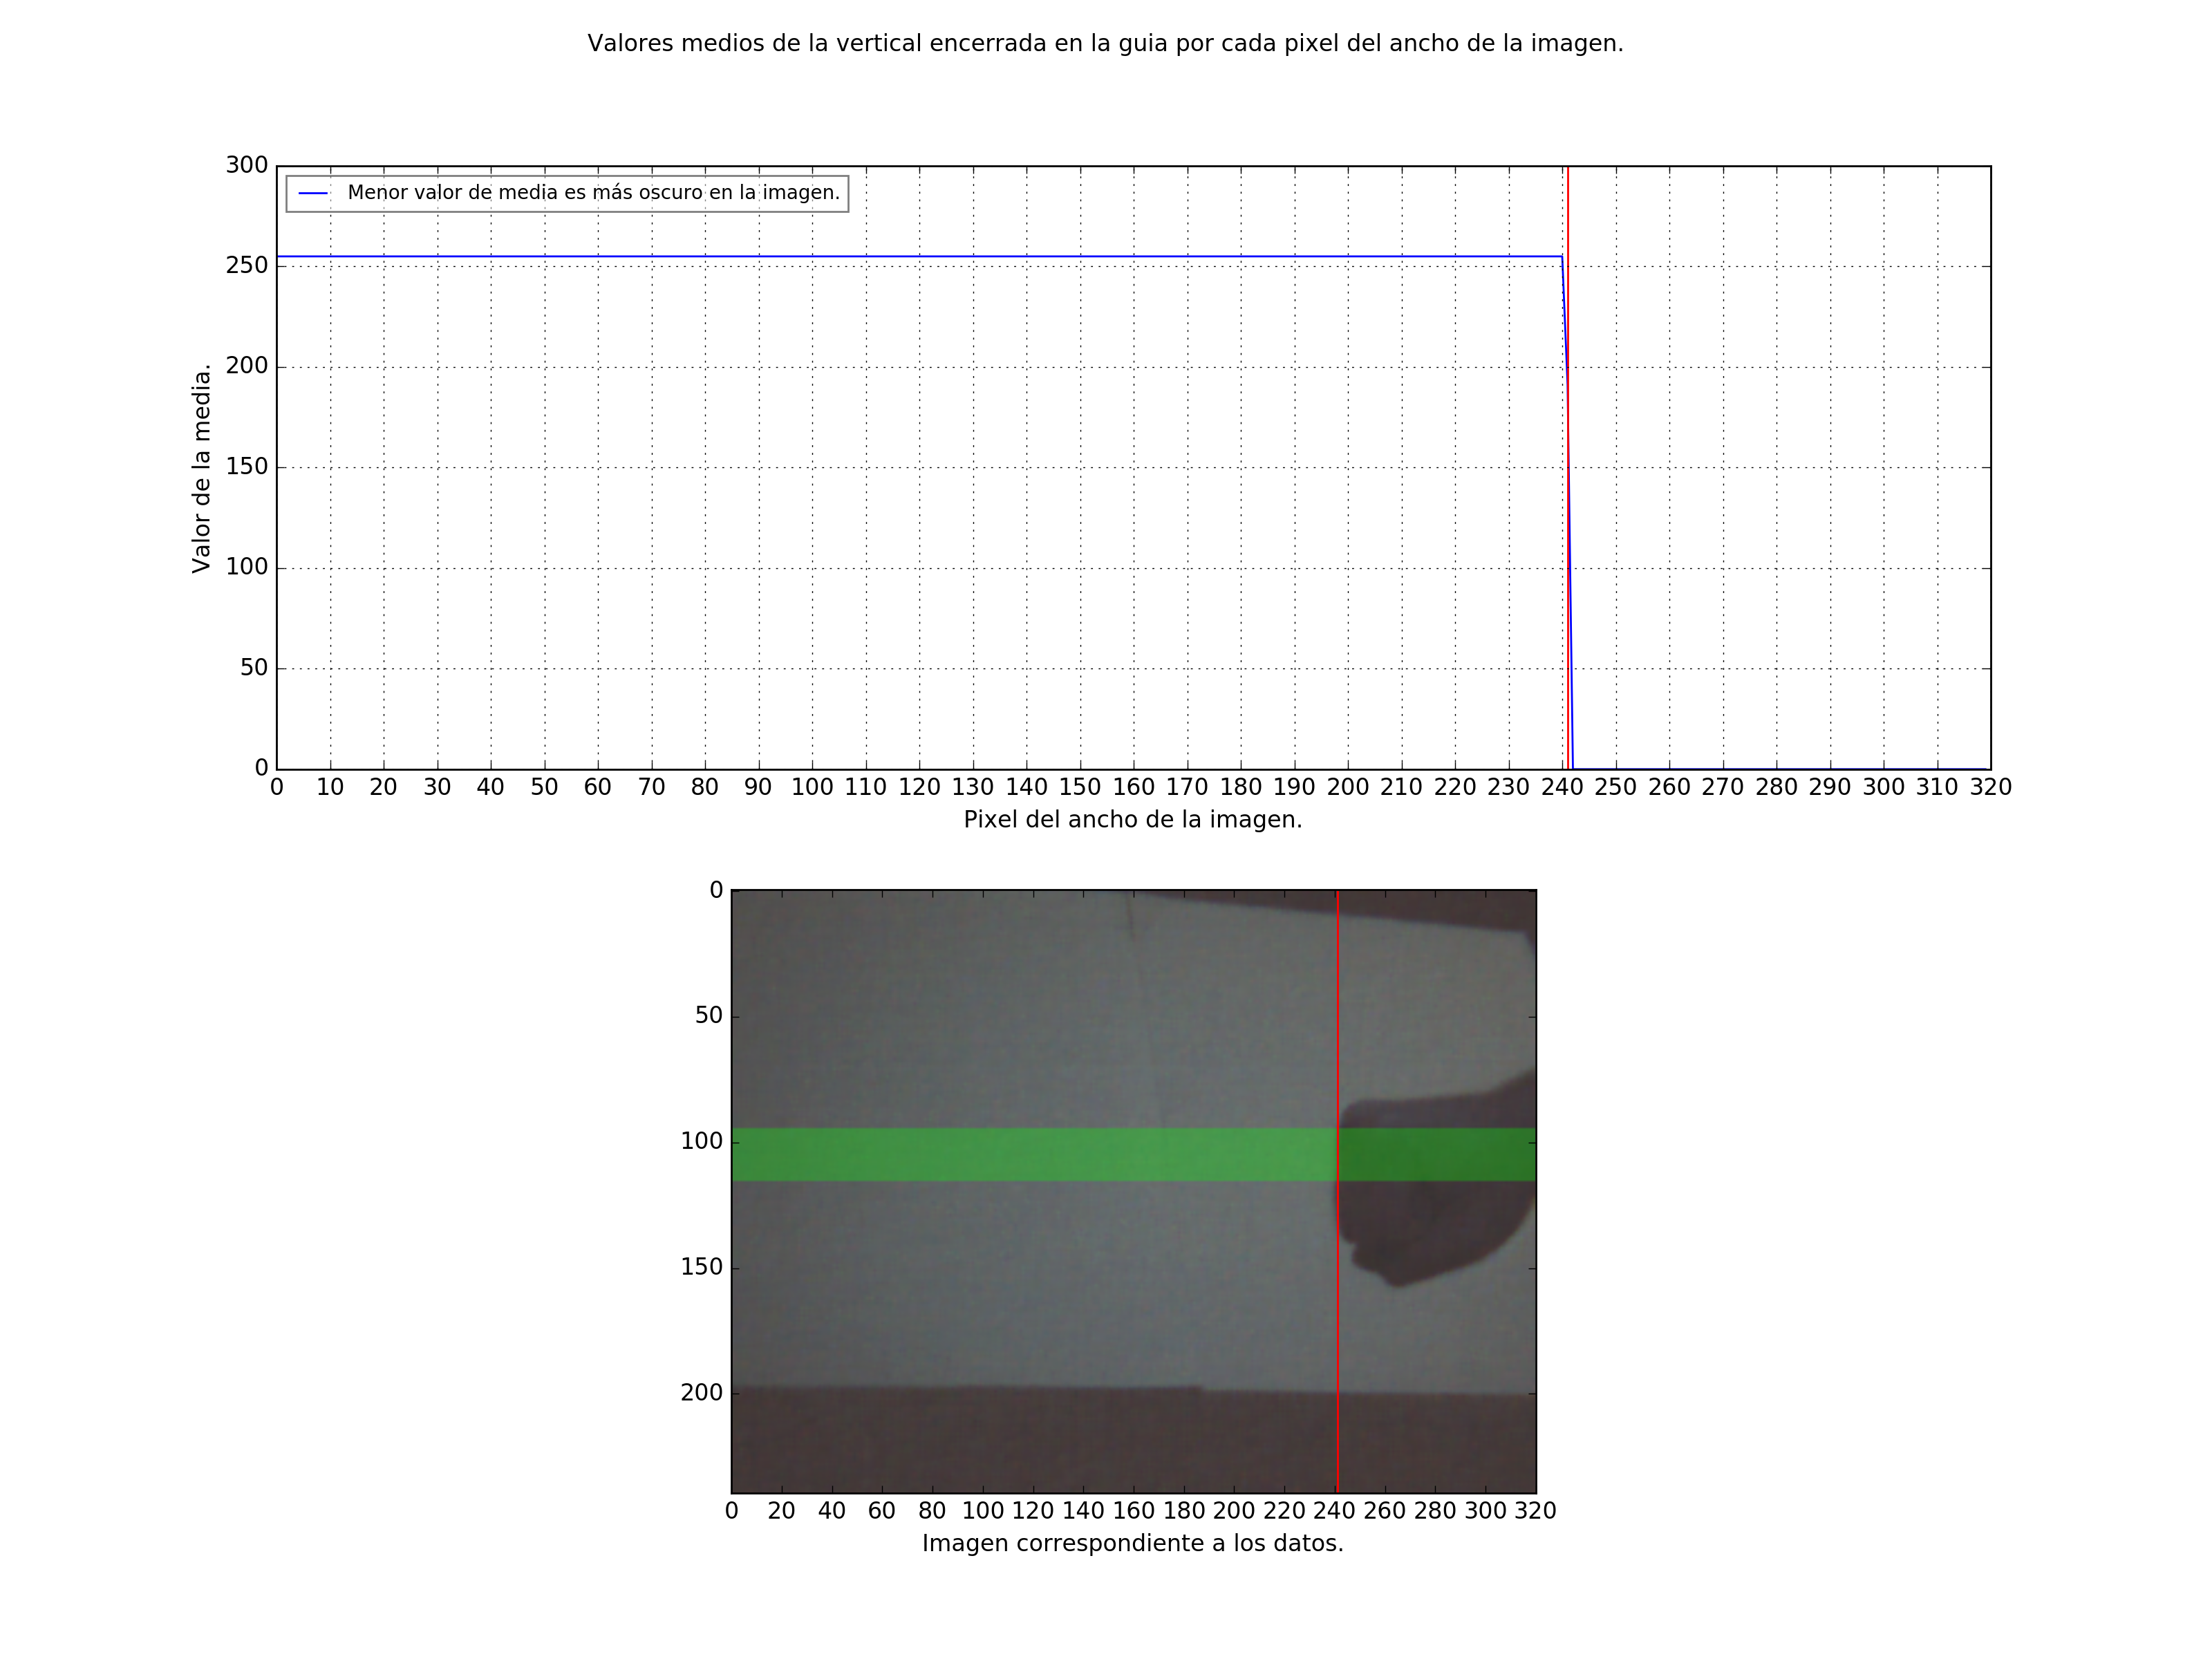
\includegraphics[width=1.8\textwidth]{Chapter4/finger-length-1}}
  \caption{El valor medio es la media de los píxeles comprendidos en la franja dado un píxel de anchura. En la gráfica vemos este valor a lo largo de toda la imagen adjunta.}
\label{fig:finger-length-1}
\end{figure}


\begin{figure}[htp]
  \makebox[\textwidth][c]{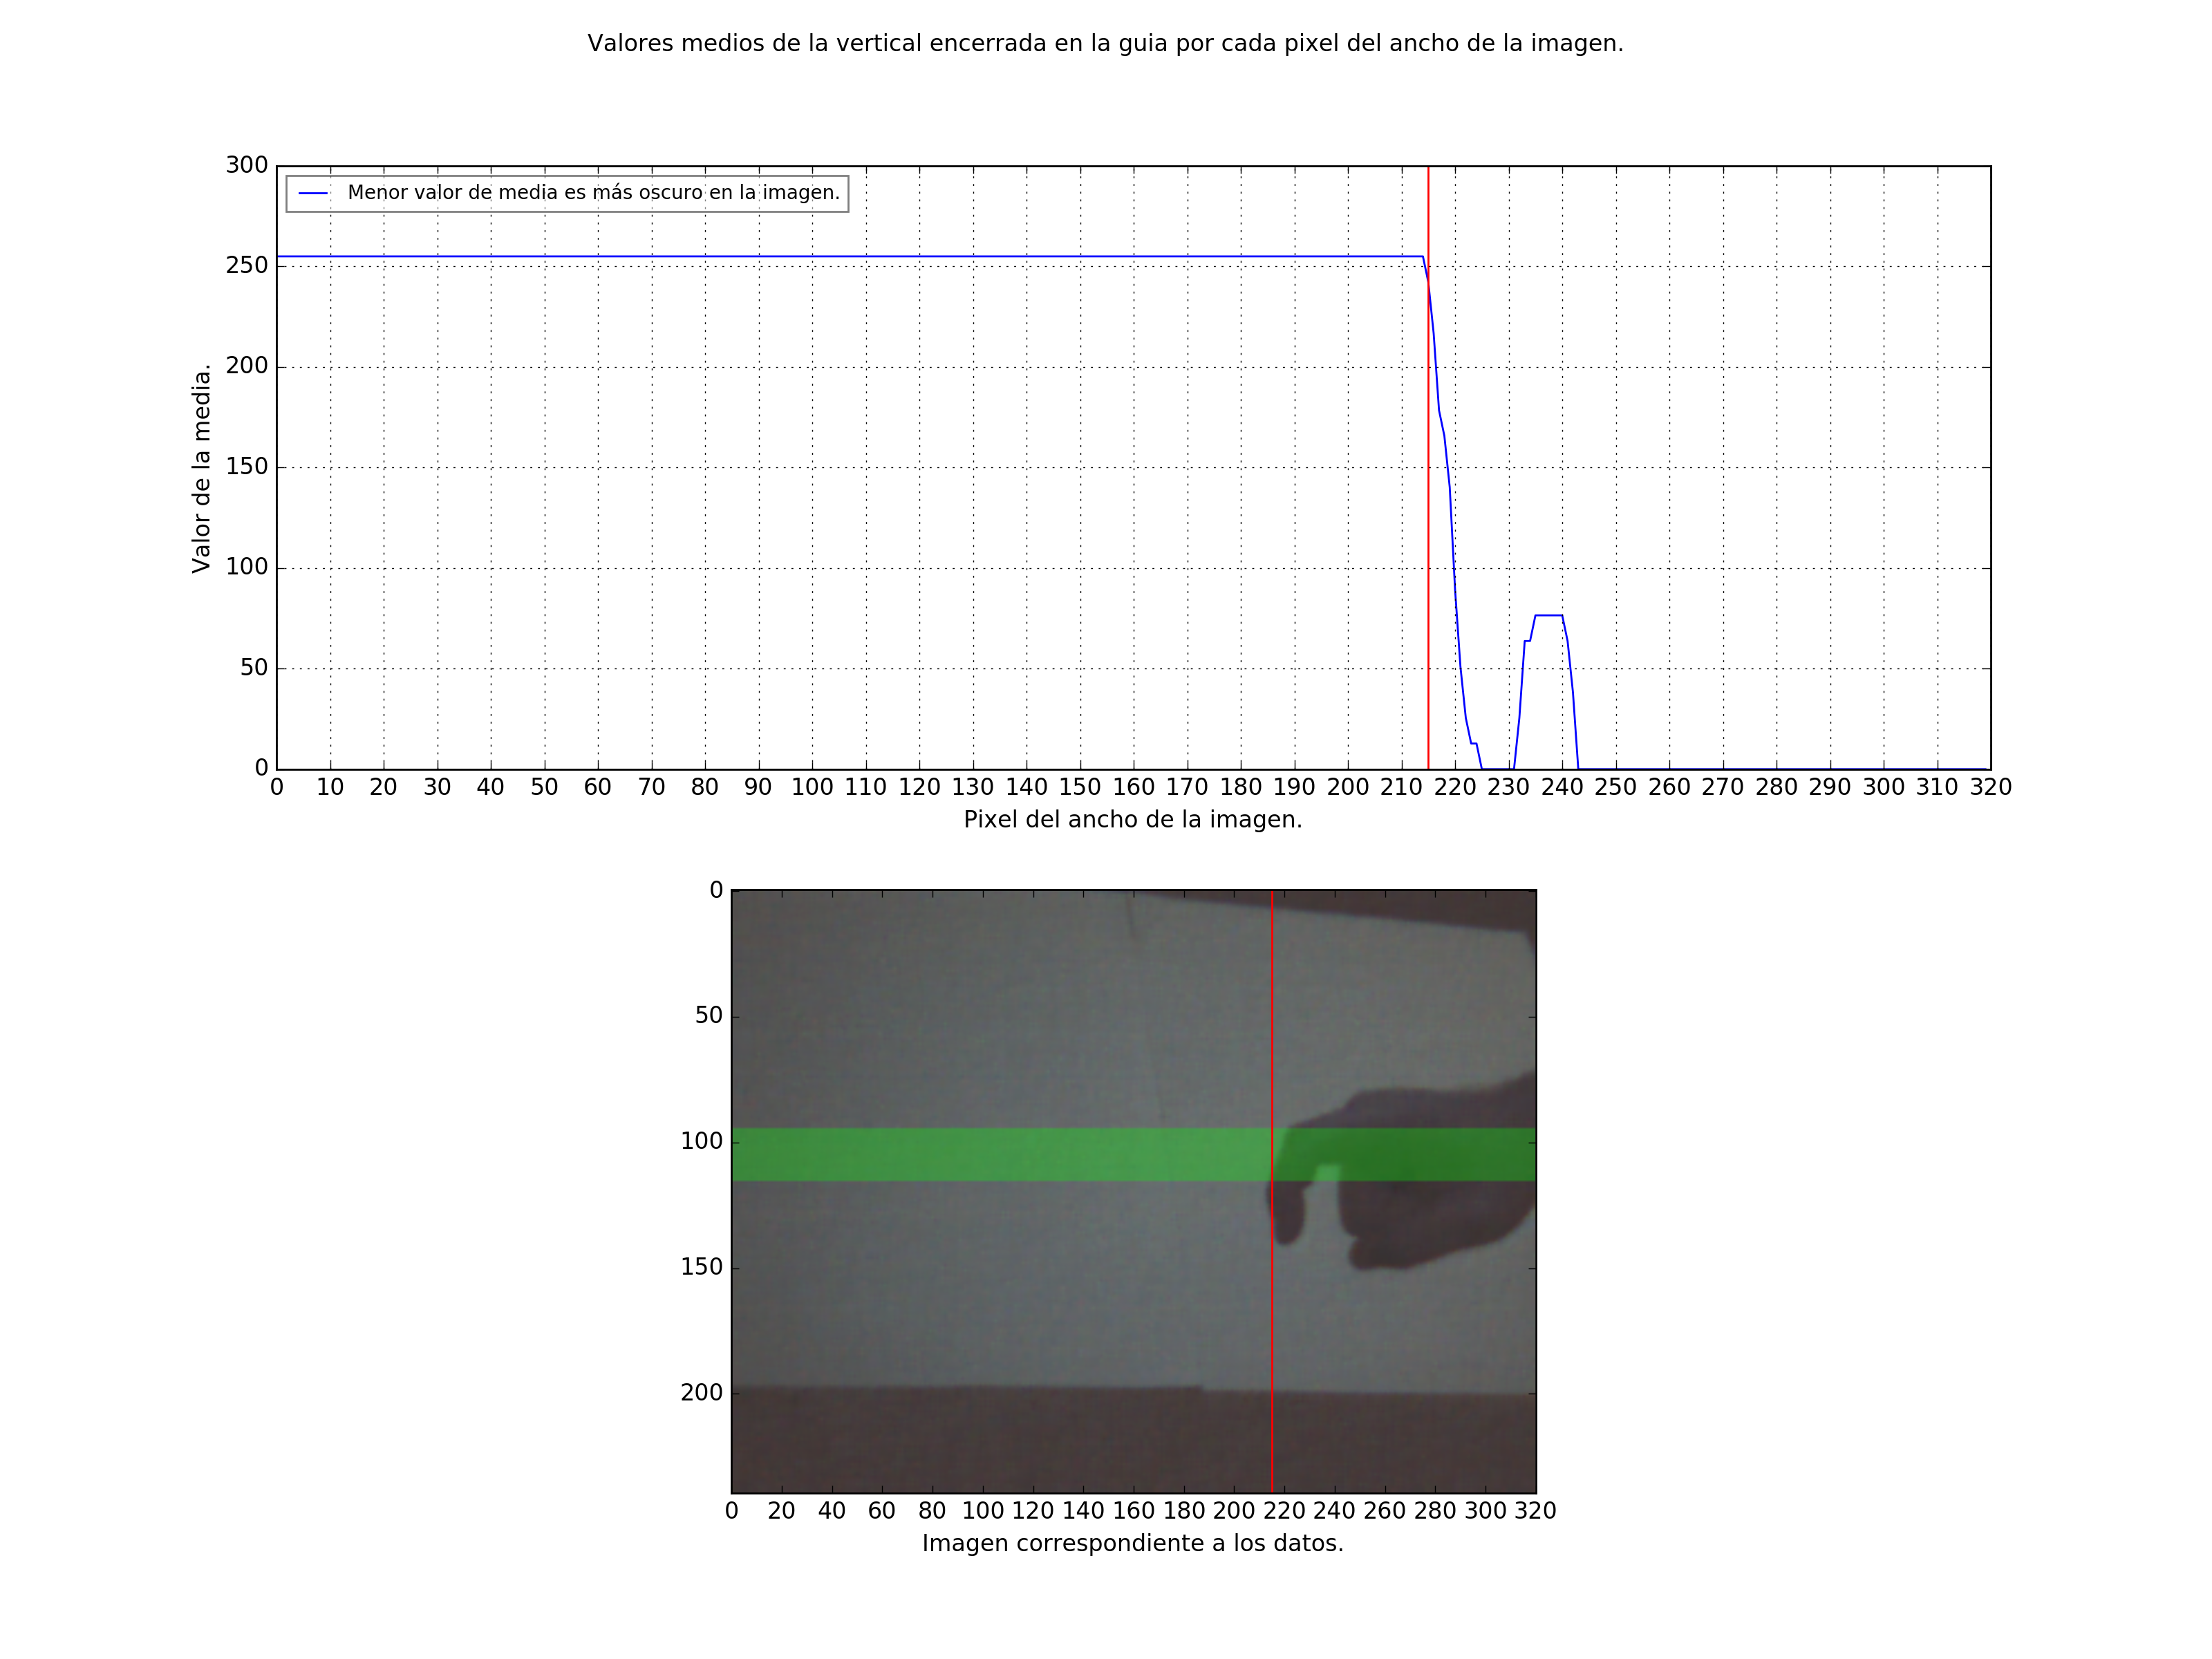
\includegraphics[width=1.8\textwidth]{Chapter4/finger-length-2}}
  \caption{Segunda muestra del código \ref{finger-length} y \ref{finger-threshold}.}
\label{fig:finger-length-2}
\end{figure}



\begin{figure}[htp]
  \makebox[\textwidth][c]{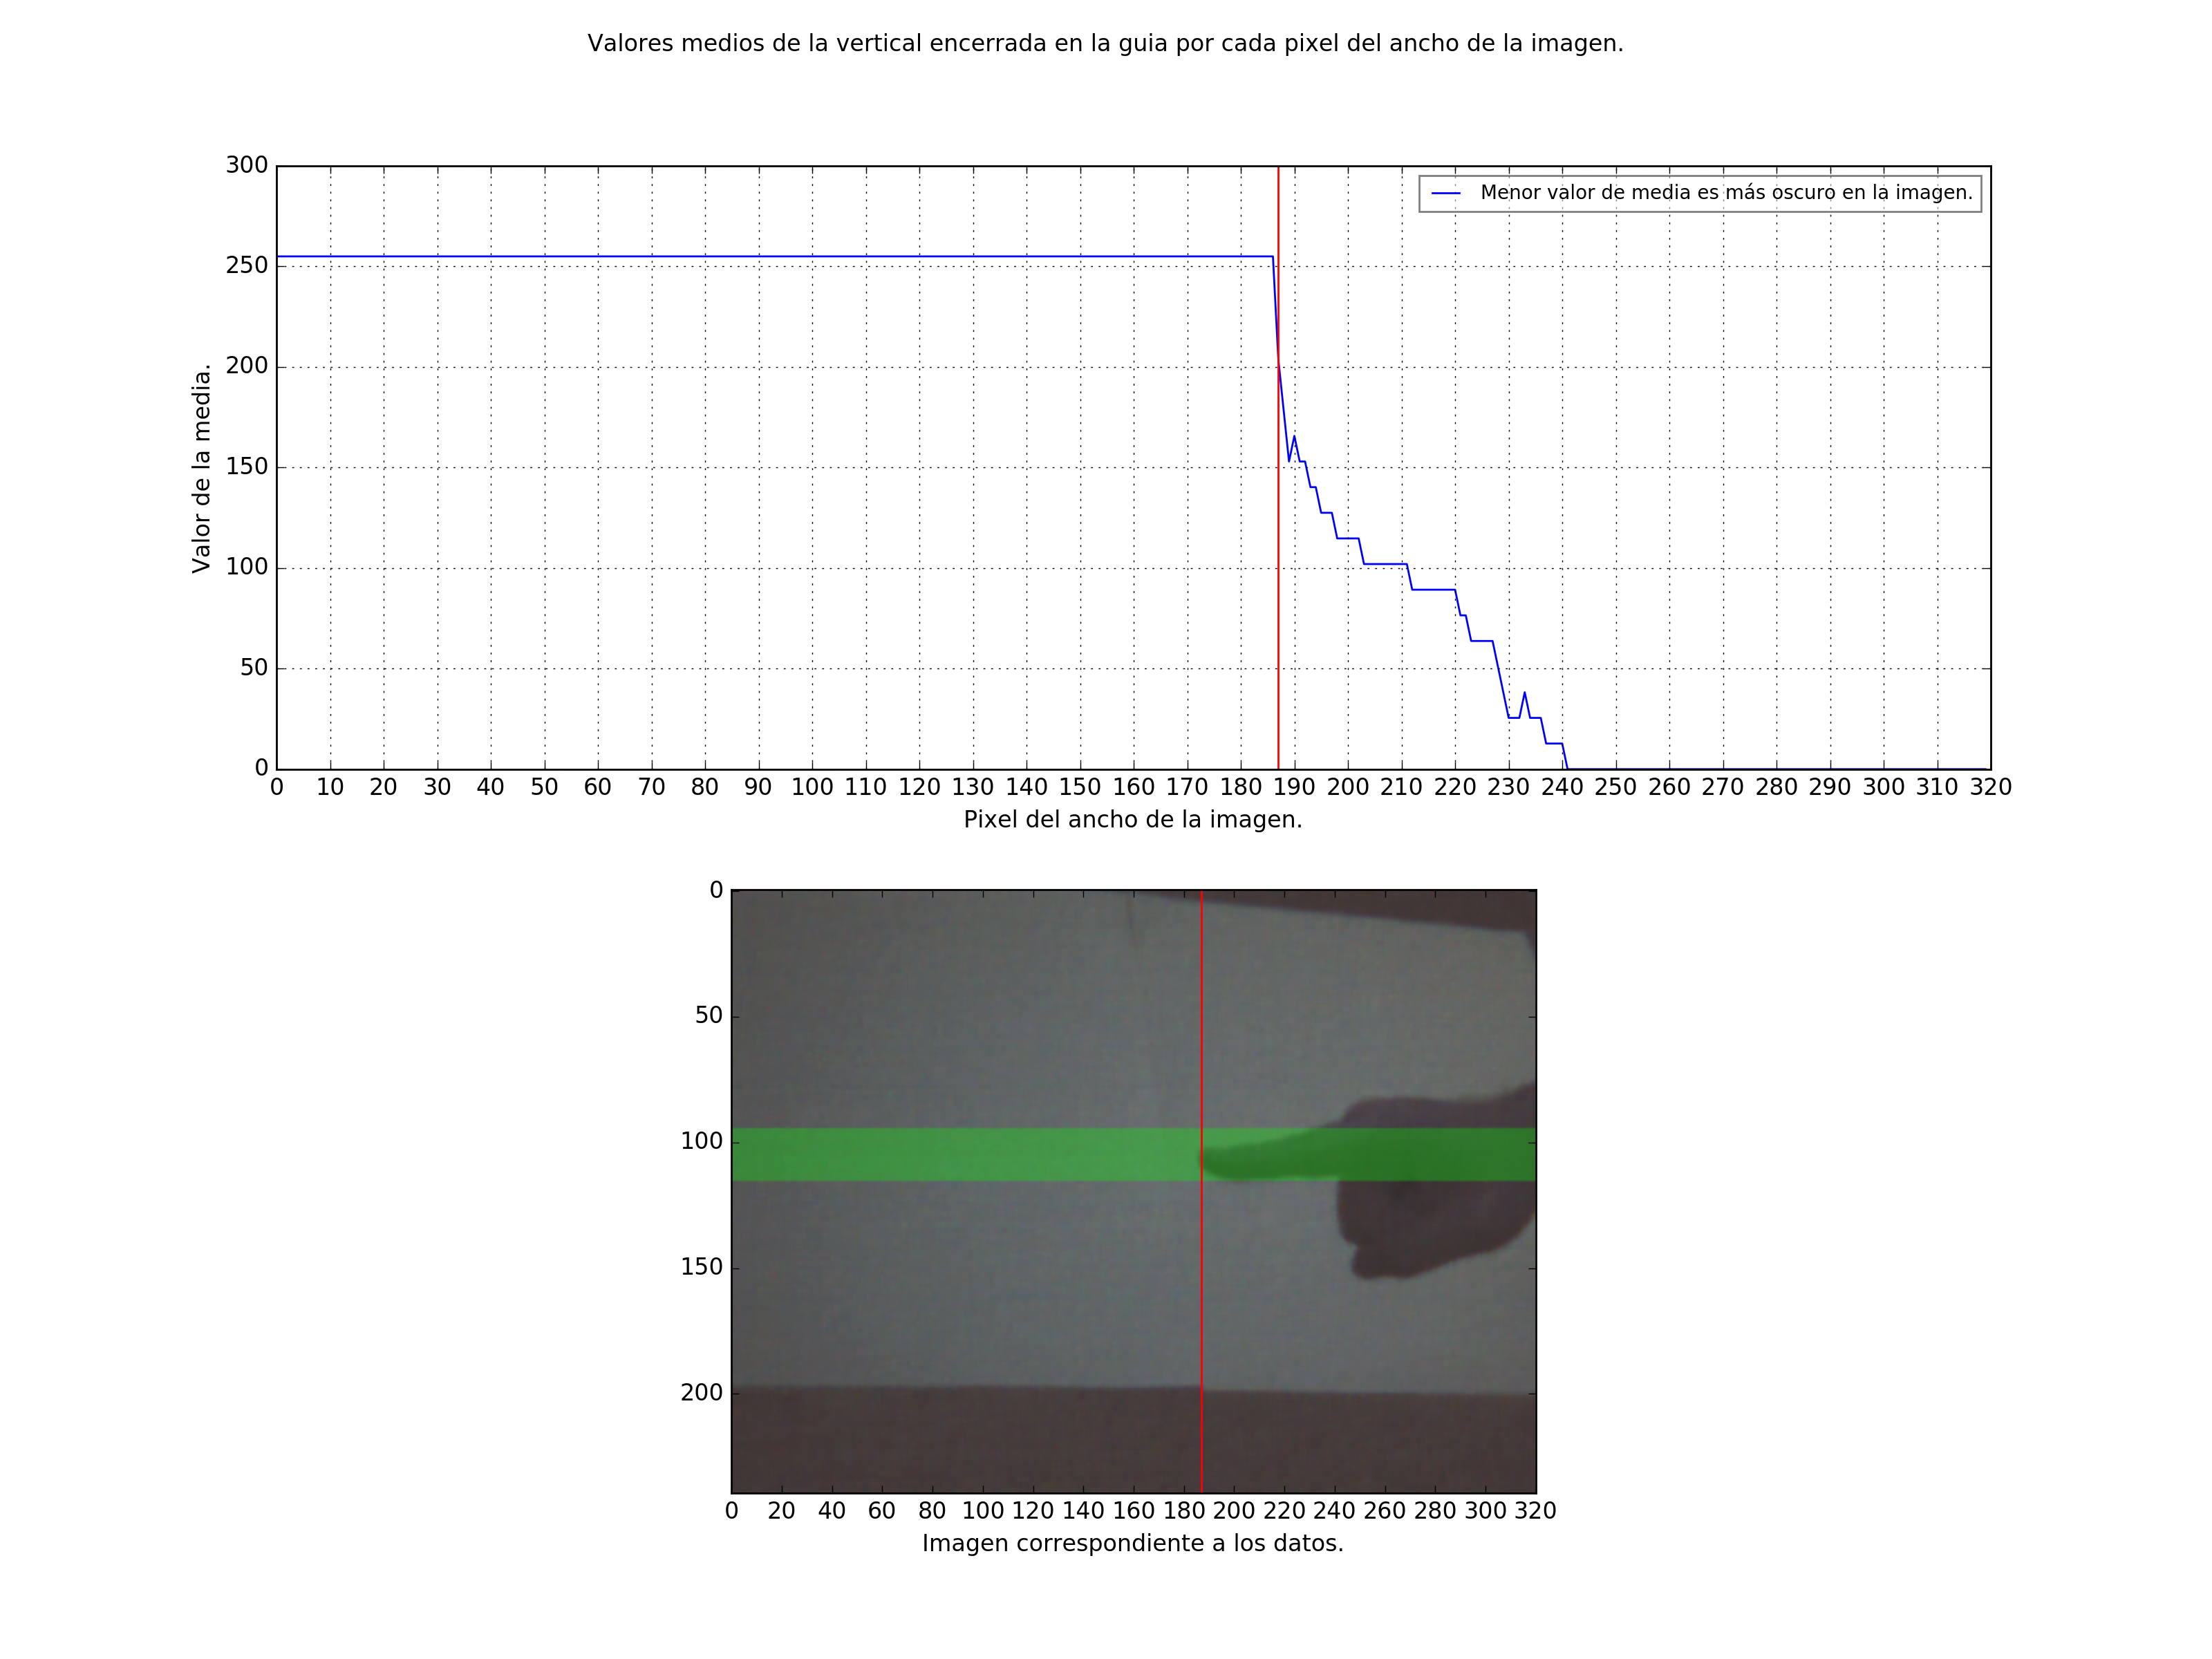
\includegraphics[width=1.8\textwidth]{Chapter4/finger-length-3}}
  \caption{Tercera y última muestra}
\label{fig:finger-length-3}
\end{figure}

\newpage


Mediante el uso de ambos \textit{scripts} obtenemos un fichero separado mediante saltos de línea de la
siguiente forma:

\begin{center}
\textit{label, (int, int, int, int, int, int, int, int)}
\end{center}

Esto es, una etiqueta (\textit{label}) que representa la longitud seguido de 8 números enteros (\textit{int}).
Las etiquetas pueden ser cualquier número entero en el rango de 0 a 5, donde 0 sería el puño cerrado y 5 sería
el dedo en extensión completa. Por otra parte, ocho valores enteros, representan la señal EMG captada por cada
uno de los 8 sensores que posee la Myo. Este fichero con los datos obtenidos de del proceso descrito en %TODO añadir referencia de dónde se explique el proceso de estirar el dedo y coger los datos
serán los datos de entrada para los algoritmos de aprendizaje automático descritos en \ref{sec:clasificación-señales-emg}.








%%%%%%%%%%%%%%%%%%%%%%%%%%%%%%%%%%%%%%%%%%%%%%%%%%%%%%%%%%%%%%%%
%
%
%
%
%        CLASIFICACIÓN DE SEÑALES
%
%
%
%
%%%%%%%%%%%%%%%%%%%%%%%%%%%%%%%%%%%%%%%%%%%%%%%%%%%%%%%%%%%%%%%%


\section{Clasificación de señales EMG}
\label{sec:clasificación-señales-emg}


Para lograr que la prótesis responda correctamente a los movimientos del usuario mediante la Myo, se ha diseñado
un modelo %TODO cambiar a plural si decido añadir más algoritmos
basado en \textit{Deep learning} %TODO añadir referencia deeplearning
utilizando las herramientas \textit{software}: \textit{nolearn} \ref{subs:nolearn}, \textit{lasagne} \ref{subs:lasagne} y \textit{scikit-learn} \ref{subs:scikit-learn}.
%TODO añadir más frameworks si añado más cosas



Para acceder al conjunto de datos de entrenamiento se ha desarrollado un programa auxiliar para ello.
Desde \textit{dataset.py} es posible recuperar los datos mediante el uso del método que podemos ver en
ref{load-dataset}.

Este método es de gran importancia puesto que la correcta carga de los datos es fundamental para el buen
funcionamiento del la red neuronal. En las líneas 6-15 se lee el fichero creado por \textit{data\_recorder.py}
\ref{data-recorder}. Como existe la posibilidad de que los datos estén ordenados de alguna forma, se debe aplicar
una permutación(líneas 18-22). Por último, se reserva una cantidad de datos fija (2000 en este caso) como conjunto
de validación (líneas 25-26). Este conjunto permite determinar la tasa de aciertos real del modelo entrenado, pues nunca formara parte del propio entrenamiento.

\begin{python}[frame=none, numbers=left,label={load-dataset}, caption={Método encargado de preparar los conjuntos de validación y entrenamiento para la red neuronal.}]
 def load_dataset():
    list_data = my_io.readFile('./Data/all_data')
    X = []
    y = []

    for data in list_data:
        y.append(eval(data[:1]))
        aux = data[4:-1].split(',')
        for i in range(len(aux)):
            aux2 = np.empty(8, dtype=np.int64)
            aux2[i] = aux[i]
        X.append(aux2)

    X = np.array(X, dtype=np.float32)
    y = np.array(y, dtype=np.int32)

    # Declare a random number generator
    rng = np.random.RandomState(seed=0)

    # Shuffle the data the right way to avoid missleading label-emg
    permutation = rng.permutation(len(X))
    X, y = X[permutation], y[permutation]

    # We reserve the last 2000 training examples for validation.
    X_train, X_val = X[:-2000], X[-2000:]
    y_train, y_val = y[:-2000], y[-2000:]

    # return all the arrays in order, as expected in main().
    return X_train, y_train, X_val, y_val

 \end{python}

Los conjuntos de datos serán utilizados por el fichero \textit{neural\_network.py} \ref{neural-network}. Este
fichero contien todo lo referente al proceso de aprendizaje, desde la construcción de la arquitectura de la red neuronal(línea 7) hasta el proceso de aprendizaje (l. 11) y la evaluación del modelo (l. 19)

\begin{python}[frame=none, numbers=left, label={neural-network},
caption={Declaración, aprendizaje y evaluación de la red neuronal}]
def main(num_epochs=500):
    # Load the dataset
    print("Loading data...")
    X, y, X_val, y_val = dataset.load_dataset_and_validationset()

    # Building the network
    nn = build_nn()

    # Begin the training phase
    tic = my_time_utils.begin()
    nn.fit(X, y)

    # Show how much time does it take the training phase
    print('Finished fitting in '
          + str(my_time_utils.elapsed_time(tic)) + 'seconds\n')

    # Show the accuracy of the model
    print('Scoring...')
    print(round(nn.score(X_val, y_val)*100, 4), '%',)

\end{python}

La arquitectura de la red neuronal \ref{nn-arquitecture} se compone de una capa de entrada, una capa de salida y de 3 capas ocultas

\begin{python}[frame=none, numbers=left, label={nn-arquitecture}, caption={Arquitectura y parámetros de la red neuronal}]
def build_nn():
    num_features = 8
    num_classes = 6

    layers = [  # 5 layers: 3 hidden layers
              ('input', InputLayer),
              ('dense0', DenseLayer),
              ('dropout0', DropoutLayer),
              ('dense1', DenseLayer),
              ('dropout1', DropoutLayer),
              ('dense2', DenseLayer),
              ('dropout2', DropoutLayer),
              ('output', DenseLayer)]
    # layer parameters:
    net = NeuralNet(layers=layers,
                    # Input
                    input_shape=(None, num_features),
                    # Dense0
                    dense0_nonlinearity=tanh,
                    dense0_num_units=200,
                    dropout0_p=0.4,
                    # Dense1
                    dense1_nonlinearity=tanh,
                    dense1_num_units=200,
                    dropout1_p=0.2,
                    # Dense2
                    dense2_num_units=200,
                    dense2_nonlinearity=tanh,
                    dropout2_p=0.2,
                    # Output
                    output_num_units=num_classes,
                    output_nonlinearity=softmax,

                    update=nesterov_momentum,
                    update_learning_rate=0.01,
                    update_momentum=0.9,

                    verbose=1,
                    on_training_finished=[report.PlotLossesAccuracy(
                                          figsize=(16, 12), dpi=200)],
                    max_epochs=500)

    return net
\end{python}

Además de la arquitectura de la red en \ref{nn-arquitecture}, podemos ver a partir de la línea 17, una
serie de parámetros. Estos parámetros configuran el comportamiento y definen cómo aprende la red neuronal:

\begin{itemize}

\item \textit{Input\_shape}: define los datos de entrada de la red. En este caso, los datos serían los 8 valores
captados por la Myo.

%TODO añadir referencia a la explicación de no linearidad
\item \textit{DenseX\_nonlinearity}: atribuye una función de activación no linear a la capa oculta \textit{X}.

\item \textit{DenseX\_num\_units}: número de unidades (neurones) que posee la capa oculta \textit{X}.

\item \textit{Update}: estas funciones afectan al cálculo del \textit{training rate} durante todo el proceso
de entrenamiento/aprendizaje.

\item \textit{{Update\_training\_rate}}: modifica el tamaño de los pasos del aprendizaje.

\item \textit{Update\_momentum}: permite suavizar los valores oscilantes de los errores.

\item \textit{Verboese}: muestra por pantalla valores como el error y los aciertos por cada iteración.

\item \textit{On\_training\_finished}: permite activar funciones o procedimientos al terminar el entrenamiento.

\item \textit{Max\_epoch}: número de iteraciones máximas que puede llevar el entrenamiento de la red.

\end{itemize}

%TODO concluir el apartado del código de la red neuronal



%%%%%%%%%%%%%%%%%%%%%%%%%%%%%%%%%%%%%%%%%%%%%%%%%%%%%%%%%%%%%%%%
%
%
%        EXPERIMENTACIÓN
%
%
%%%%%%%%%%%%%%%%%%%%%%%%%%%%%%%%%%%%%%%%%%%%%%%%%%%%%%%%%%%%%%%%

\newpage

\section{Experimentación}
\label{sec:experimentación}


Las redes neuronales pueden llegar a alcanzar millones de hiper-parámetros \cite{NovikovPOV15} y es necesario
probar diversas calibraciones. En esta sección se expondrán las pruebas realizadas con la red neuronal definida
en \ref{nn-arquitecture}.

El primer parámetro a probar será \textit{update} sin modificar ningún otro de los parámetro descritos en \ref{nn-arquitecture}. Los resultados que se muestran en \ref{tab:update} son los resultados del aprendizaje sobre el
conjunto de datos de validación


\begin{table}[htp]
\caption{Porcentaje de aciertos obtenido usando el conjunto de entrenamiento según el algoritmo utilizado como
\textit{update}. El mejor resultado está marcado en negrita.}
\label{tab:update}
\centering
\begin{tabular}{l c c c c}
\toprule
& \textbf{rmsprop} & \textbf{adagrad} & \textbf{nesterov-momentum}  &   \textbf{adam}  \\
\midrule
Tasa de aciertos (\%) & 47.25 & 52.89 & \textbf{58.25} & 48.96   \\
\bottomrule\\

\end{tabular}
\end{table}


\begin{table}[htp]
\label{tab:aciertos}
\centering
\begin{tabular}{l c c c c }
\toprule
 & \textbf{momentum} &  \textbf{sgd}  &  \textbf{adamax}  & \textbf{adadelta}\\
\midrule
Tasa de aciertos (\%) & 56.50 & 48.84 & 56.90 & 47.08 \\
\bottomrule\\

\end{tabular}
\end{table}



En las siguientes pruebas se utilizará \textit{nesterov-momentum} como función de actualización por haber conseguido la mayor tasa de aciertos (58.25\%). 

Cada una de las capas ocultas de la red puede implementar una función de activación no lineal\cite{nonlinearities}. La tabla \ref{tab:nonlinearities} es el resultado de aplicar \textit{grid search} sobre las funciones \textit{verify, tanh y sigmoid} en cada capa oculta de la red neuronal. De ella, se puede extraer que la combinación \textit{rectify-rectify-rectify} es la que presenta mejores resultados (40.36\%)

\begin{table}[htp]
\caption{Porcentaje de aciertos sobre el conjunto de entrenamiento mediante la permutación de las funciones \textit{verify}, \textit{tanh} y \textit{sigmoid}. En negrita se marca el mejor resultado.}
\label{tab:nonlinearities}
\centering
\begin{tabular}{c c c c c}

\toprule
\textbf{Capa oculta 1} & \textbf{Capa oculta 2} & \textbf{Capa oculta 3} & \textbf{Precisión (\%)} & \textbf{std} \\
\midrule
tanh & tanh & tanh & 52.16 & 0.00563   \\
tanh & sigmoid & tanh & 51.51 & 0.00660   \\
tanh & rectify & tanh & 54.53 & 0.00794   \\
tanh & tanh & sigmoid & 47.81 & 0.00565   \\
tanh & sigmoid & sigmoid & 46.35 & 0.01223   \\
tanh & rectify & sigmoid & 50.89 & 0.00871   \\
tanh & tanh & rectify & 52.91 & 0.00671   \\
tanh & sigmoid & rectify & 52.64 & 0.00696   \\
tanh & rectify & rectify & 55.91 & 0.00858   \\
sigmoid & tanh & tanh & 46.30 & 0.01287   \\
sigmoid & sigmoid & tanh & 46.02 & 0.01117   \\
sigmoid & rectify & tanh & 49.95 & 0.00885   \\
sigmoid & tanh & sigmoid & 43.9 & 0.00864   \\
sigmoid & sigmoid & sigmoid & 41.81 & 0.00656   \\
sigmoid & rectify & sigmoid & 46.51 & 0.01078   \\
sigmoid & tanh & rectify & 47.44 & 0.00752   \\
sigmoid & sigmoid & rectify & 46.31 & 0.01228   \\
sigmoid & rectify & rectify & 51.21 & 0.00854   \\
rectify & tanh & tanh & 49.98 & 0.00526   \\
rectify & sigmoid & tanh & 50.31 & 0.00916   \\
rectify & rectify & tanh & 54.37 & 0.00501   \\
rectify & tanh & sigmoid & 49.09 & 0.01037   \\
rectify & sigmoid & sigmoid & 46.23 & 0.00888   \\
rectify & rectify & sigmoid & 51.22 & 0.00635   \\
rectify & tanh & rectify & 55.07 & 0.01142   \\
rectify & sigmoid & rectify & 51.54 & 0.00993   \\
\textbf{rectify} & \textbf{rectify} & \textbf{rectify} & \textbf{56.77} & \textbf{0.00961}   \\


\bottomrule\\
\end{tabular}
\end{table}





\newpage






El siguiente experimento se realizará sobre el parámetro que controla el número de unidades (neuronas) de cada una de las capas ocultas de la red neuronal y el parámetro \textit{dropout} \ref{subs:dropout}:

\begin{itemize}

	\item Perfil bajo: 200 neuronas por capa y 0.2 de \textit{dropout}.

	\item Perfil intermedio: 1200 neuronas por capa y 0.4-0.5 de \textit{dropout}.

	\item Perfil alto: 10000 neuronas por capa y 0.8-0.9 de \textit{dropoout}.

\end{itemize}


\begin{table}[htp]
\caption{Experimentación con el número de unidades (neuronas) y \textit{dropout}. Marcado en negrita está el mejor resultado.}
\centering
\begin{tabular}{l c c c}
\toprule
& \textbf{Neuronas} & \textbf{Dropout} & \textbf{Precisión de validación (\%)} \\
\midrule
\textbf{Perfil bajo}  & 200   &  0.2  & 55.25  \\
\textbf{Perfil medio} & \textbf{1200}  &  \textbf{0.4}  & \textbf{61.10}  \\
\textbf{Perfil alto}  & 4500  &  0.8  & 45.05  \\

\bottomrule\\

\end{tabular}
\label{tab:perfil}
\end{table}


En la tabla \ref{tab:perfil} el perfil alto usa 4500 neuronas cuando debería ser una prueba con 10000
o más neuronas, esto es debido a limitaciones de la tarjeta gráfica del equipo utilizado para las pruebas (NVIDIA GT 540M).


En la columna de precisión de validación, podemos ver la tasa de aciertos que logra el modelo con datos con los que
no ha sido entrenado. Vemos que un mayor número de neuronas no implica una mayor tasa de aciertos, pero se puede observar que 1200 neuronas con 0.4 de \textit{dropout} funcionan mejor que 200 neuronas con 0.2 de \textit{dropout}.
La configuración del perfil medio es la que se usará en la siguiente y última prueba.


El último parámetro a probar es el \textit{learning rate}, la tabla \ref{tab:learning-rate}

\begin{table}[htp]
\caption{Experimentación con el parámetro \textit{learning rate}. En negrita se marca el mejor resultado.}
\centering
\begin{tabular}{c c}
\toprule
\textbf{Learning rate} &  \textbf{Precisión de validación (\%)} \\
\midrule
  0.1    &  44.00  \\
  \textbf{0.01}   &  \textbf{61.10}  \\
  0.001  &  43.25  \\

\bottomrule\\

\end{tabular}
\label{tab:learning-rate}
\end{table}







\newpage




\subsection{Modelo final}

Tras el proceso de experimentación, los parámetros que se usarán en el apartado de resultados (\ref{subs:resultados}) son los que se muestran a continuación en \ref{parametros-finales}.

\begin{python}[frame=none, numbers=left, label={parametros-finales}, caption={Configuración de las capas de la red neuronal y sus parámetros finales marcados en negrita}]
num_features = 8
num_classes = 6

layers = [  # 5 layers: 3 hidden layers
          ('input', InputLayer),
          ('dense0', DenseLayer),
          ('dropout0', DropoutLayer),
          ('dense1', DenseLayer),
          ('dropout1', DropoutLayer),
          ('dense2', DenseLayer),
          ('dropout2', DropoutLayer),
          ('output', DenseLayer)]
# layer parameters:
net = NeuralNet(layers=layers,
                # Input
                input_shape=(None, num_features),
                # Dense0
                dense0_nonlinearity=rectify,
                dense0_num_units=1200,
                dropout0_p=0.4,
                # Dense1
                dense1_nonlinearity=rectify,
                dense1_num_units=1200,
                dropout1_p=0.4,
                # Dense2
                dense2_num_units=1200,
                dense2_nonlinearity=rectify,
                dropout2_p=0.4,
                # Output
                output_num_units=num_classes,
                output_nonlinearity=softmax,

                update=nesterov_momentum,
                update_learning_rate=0.01,

                max_epochs=500)
\end{python}

\subsection{Resultados}
\label{subs:resultados}

El rendimiento del modelo, como se ha explicado anteriormente, se determinará mediante el conjunto de validación
compuesto por 2000 de los 26540 conjunto total de datos disponibles. Remarcar de nuevo, que este grupo de datos no
ha sido utilizado en ningún momento en el proceso de aprendizaje, por lo cual, todos los datos son nuevos para el
modelo.

El primer resultado se muestra en la figura \ref{fig:confusion-matrix}. Esta matriz permite ver de forma gráfica el
resultado de las predicciones. A la matriz le acompaña una barra de colores, donde el color más cálido (marrón en
este caso) indica una mayor tasa de coincidencia de índices columna-fila. En contraposición, el color frío indica
un menor ratio. Idealmente, la matriz debería mostrar en su diagonal secundaria los tonos cálidos, indicando que las predicciones son correctas.


\begin{figure}[htp]
  \centering
    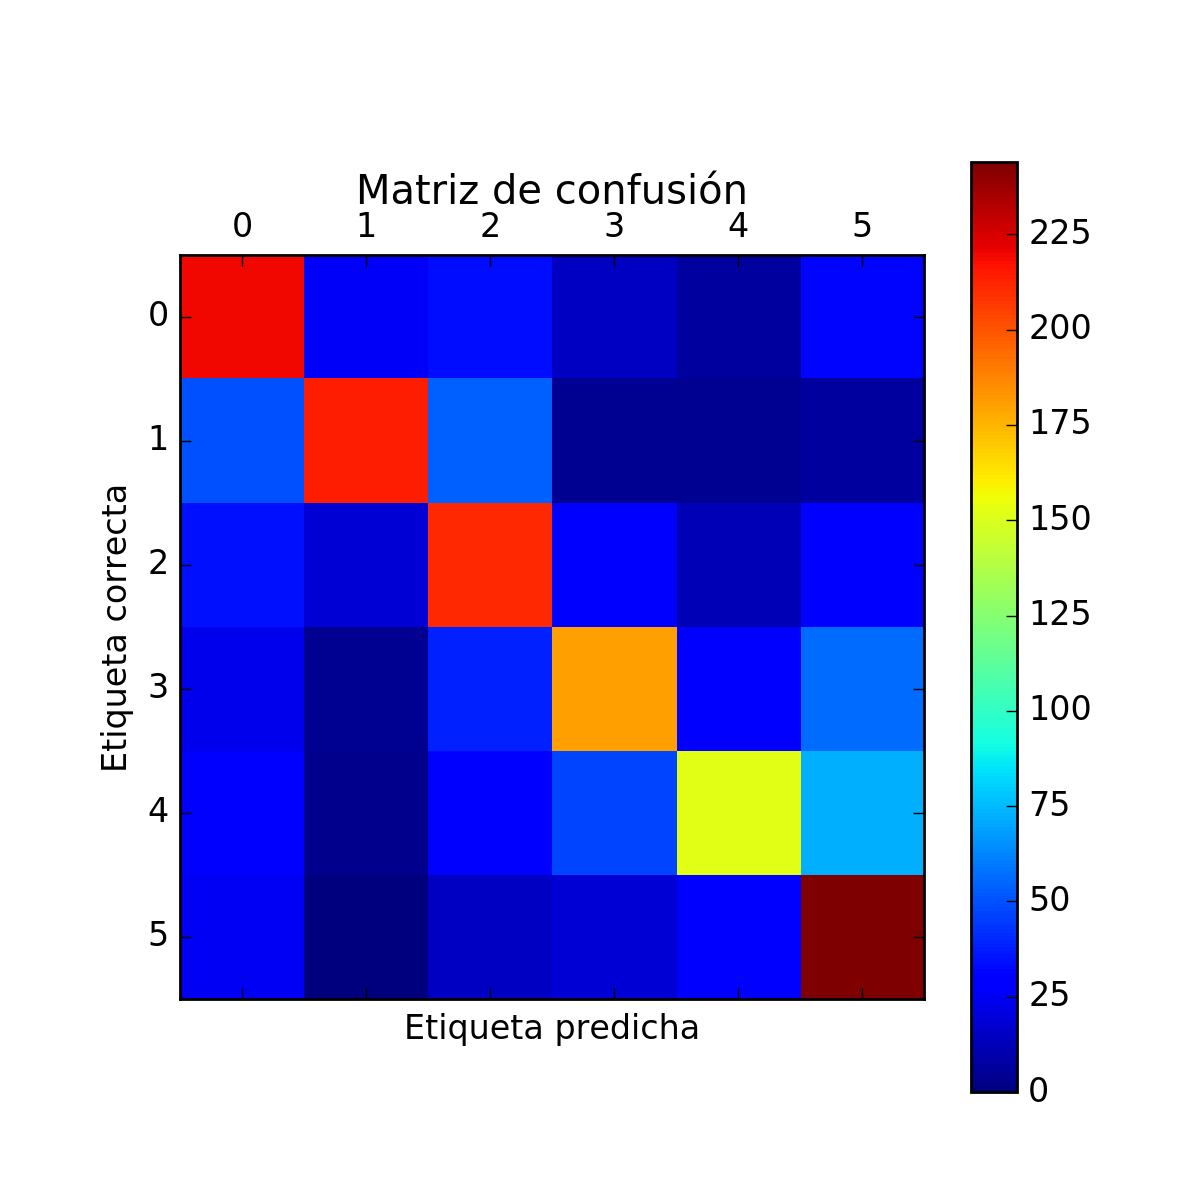
\includegraphics[width=0.8\textwidth]{Chapter4/ultimo-test-matriz}
  \caption{Matriz de confusión del modelo de red neuronal final.}
\label{fig:confusion-matrix}
\end{figure}

La precisión de un modelo no debe ser nunca el único indicador de calidad o rendimiento de un modelo de aprendizaje,
puesto que en ámbitos como el de, por ejemplo, la medicina obtener un falso positivo o un falso negativo, puede ser un grave error. Por ello, se ha incluido un informe con datos sobre además de la precisión, las medidas de exhaustividad (\textit{recall}, en inglés) que mide el verdadero ratio de positivos (es el verdaderos positivos dividido por los verdaderos positivos y falsos negativos)  y valor-F (\textit{F1 score}, en inglés) que es una media entre la exhaustividad y la precisión, concretamente se mide como:

\begin{equation}
2*\frac{Precisi\acute{o}n*Exhaustividad}{Precisi\acute{o}n+Exhaustividad}
\end{equation}



\begin{table}[htp]
\caption{Tabla con un resumen de distintos criterios de evaluación sobre los aciertos de cada etiqueta.}
\label{tab:report}
\centering
\begin{tabular}{l c c c}

\toprule
	&	\textbf{Precisión}	&	\textbf{Exhaustividad}		& \textbf{Valor-F} \\
\midrule
Etiqueta 0		&	0.57	&	0.66	&	0.61			\\
Etiqueta 1		&	0.80	&	0.64	&	0.71		\\
Etiqueta 2		&	0.55	&	0.63	&	0.59		\\
Etiqueta 3		&	0.61	&	0.54	&	0.58		\\
Etiqueta 4		&	0.65	&	0.46	&	0.54		\\
Etiqueta 5		&	0.55	&	0.73	&	0.63		\\
\midrule
\textbf{Media}		&	0.62	&	0.61	&	0.61		\\
\bottomrule\\
\end{tabular}
\end{table}

\chapter{Conclusiones} % Main chapter title
\label{Chapter5}

\chapquote{En este capítulo se resumirá el alcance que ha tenido el proyecto. En el apartado \ref{sec:conclusiones} se hace una reflexión sobre los resultado obtenidos en \ref{sec:experimentación}. En el apartado \ref{sec:trabajo-futuro} se muestran algunas ideas que se han quedado por desarrollar o errores que se han podido por corregir.}




%%%%%%%%%%%%%%%%%%%%%%%%%%%%%%%%%%%%%%%%%%%%%%%%%%%%%%%%%%%%%%%%
%
%
%        Conclusiones
%
%
%%%%%%%%%%%%%%%%%%%%%%%%%%%%%%%%%%%%%%%%%%%%%%%%%%%%%%%%%%%%%%%%

\section{Conclusiones}
\label{sec:conclusiones}

Se ha logrado desarrollar un modelo de red neuronal artificial que resuelve el problema de clasificación con una precisión ligeramente superior al 60\%. En el apartado \ref{subs:resultados} del capítulo \ref{Chapter4} se puede comprobar gráficamente el rendimiento de las predicciones.

El resultado, aunque no es perfecto ni es el que se esperaba obtener, es satisfactorio puesto que el desarrollo de 
un proyecto de estas características requiere que cada etapa del mismo, sea realizada con precisión y de forma 
robusta, es decir, tanto la etapa de obtención del conjunto de trabajos y la etapa de clasificación requieren una 
atención y un desarrollo mayor del que se le ha podido dar en este trabajo principalmente por límites de tiempo y 
por la complejidad del estudio de las áreas de la ingeniería de datos y el aprendizaje automático respectivamente.

Por otra parte, se ha conseguido una prótesis como parte del entorno de pruebas para el algoritmo desarrollado 
dentro de un presupuesto ajustado (anexo \ref{presupuestoProyecto}, que debido al rendimiento del algoritmo y el 
tiempo dedicado al desarrollo del mismo, solo se ha podido hacer pruebas básicas con los motores.

Puesto que en general, el desarrollo y los resultados han sido satisfactorios teniendo en cuenta las limitaciones 
anteriores, se espera seguir desarrollando este trabajo como Proyecto Final en el Máster de Automática y Robótica 
con el fin de perfeccionar el trabajo realizado hasta ahora y conseguir mejores resultados respecto al 
funcionamiento del algoritmo de clasificación.

En el siguiente apartado (\ref{sec:trabajo-futuro}) se deja constancia de las principales ideas que se han quedado fuera de este trabajo.


%Por ello, y como se menciona en el siguiente apartado, para mejorar el resultado es necesario primero construir un conjunto de datos más robusto y balanceado. Una vez solventado este problema, el proceso de experimentación podría dar lugar a distintas configuraciones de parámetros que darían lugar a un modelo más robusto, pudiendo hacer uso de las mismas herramientas usadas y desarrolladas en este trabajo. En el apartado \ref{sec:trabajo-futuro} se incluyen consejos sobre técnicas que no se han podido probar para la búsqueda óptima de parámetros para las redes neuronales.

%Con los resultados mostrados y sus reflexiones, se ha logrado dejar constancia del largo proceso que supone no solo 
%el desarrollo de \textit{software} para realizar tareas de clasificación sino también la de construir tu propio 
%conjunto de datos \dots


%%%%%%%%%%%%%%%%%%%%%%%%%%%%%%%%%%%%%%%%%%%%%%%%%%%%%%%%%%%%%%%%
%
%
%        Trabajo futuro
%
%
%%%%%%%%%%%%%%%%%%%%%%%%%%%%%%%%%%%%%%%%%%%%%%%%%%%%%%%%%%%%%%%%

\section{Trabajo futuro}
\label{sec:trabajo-futuro}

Con el fin de mejorar los resultados obtenidos en este trabajo y debido a limitaciones de tiempo, estas son algunas ideas y pruebas que se pueden realizar.

Al tratarse de un conjunto de datos propio, es decir, uno que se ha creado para este propósito y no un conjunto que se encuentran en la mayoría de artículos \cite{krizhevsky2009learning, lecun1998mnist, netzer2011reading}, es posible que no se pueda obtener una tasa de aciertos perfecta (u óptima) por ello se han de aplicar técnicas de ingeniería de datos para demostrar si es posible conseguir una mejora o no. Aumentar el tamaño del conjunto de datos y conseguir que el dicho conjunto esté balanceado deberían ser las primeras mejoras que implementar.


Alternativas al \textit{grid search} para encontrar los mejores parámetros con el que entrenar las redes neuronales.
\textit{Grid search} realiza una búsqueda mediante fuerza bruta para encontrar los parámetros que consigan los 
mejores resultados, con miles de posibles parámetros que pueden aprenderse, el tiempo de entrenar modelos mediante 
esta búsqueda y con equipos de bajo rendimiento tiende a ser impracticable. Algunas alternativas a esta situación 
sería el uso de \textit{random search} o \textit{bayesian optimizations}.





%----------------------------------------------------------------------------------------
%   THESIS CONTENT - APPENDICES
%----------------------------------------------------------------------------------------

\appendix % Cue to tell LaTeX that the following "chapters" are Appendices

% Include the appendices of the thesis as separate files from the Appendices folder
% Uncomment the lines as you write the Appendices

% Appendix A



\chapter{Presupuesto del proyecto} % Main appendix title
\label{presupuestoProyecto}

\pagestyle{empty}

\begin{landscape}

\begin{table}
\caption{Lista de los componentes utilizados}
\label{tab:presupuesto}
\centering

\begin{tabular}{l l c c c}
\toprule
\textbf{Componente} & \textbf{Especificación} & \textbf{Cantidad} & \textbf{Precio unitario (\euro)} & \textbf{Precio total (\euro)} \\
\midrule
 Rodamiento                 & 10mm diámetro exterior, 3mm de interior; 4mm de ancho & 14  & 0.15 & 2.10 \\
 Rodamiento en V            & 12mm - 9.5mm díametro exterior, 3mm de interior, 4mm de ancho & 10 & 0.20 & 2 \\
 Tornillo cabeza plana      & Métrica 2m, 6 mm de largo & 14  & 0.15 & 2.10 \\
 Tornillo cabeza estrella   & Métrica 2m, 6 mm de largo & 20  & 0.15 & 3 \\
 Tornillo prisionero        & Métrica 2, 3mm de largo & 6 & 0.09 & 0.55 \\
 Tornillo                   & Métrica 3, 45mm de largo & 4 & 0.23 & 0.92 \\
 Tuerca M2                  & Métrica 2  &  30  & 0.10 & 3.00 \\
 Tuerca M3                  & Métrica 3  &  30  & 0.10 & 3.00 \\
 Muelle                     & 4.5mm diámetro exterior, 20mm longitud &  10  &  0.29  &  2.90 \\
 Motor corriente continua   & 16 mm diámetro, 50 mm largo, 120rpm & 5 & 25.2 & 126  \\
 Micro servo                & Estándar 9g & 1 & 1.34 & 1.34 \\
 Clavija/tarugo de metal    & 3mm diámetro, 12mm largo & 10  &  0.15 & 1.50  \\
 Clavija/tarugo de metal    & 3mm diámetro, 14mm largo & 10  &  0.15 & 1.50  \\
 Clavija/tarugo de metal    & 3mm diámetro, 6mm largo &  10  &  0.06 & 0.60  \\
 Virola doble               & 0.8mm de díametro interior & 10 & 0.07 & 0.70  \\
 Cable de metal             & 0.7mm de díametro & 5 (metros) &  0.28 & 1.40  \\
 Plástico                   & Unos 300g (si te sale a la primera) & 0.3 (Kg) & 20.0 & 6.0 \\
 Arduino UNO                & & 1 & 19.90 & 19.90   \\
 Adafruit Motor Shield      & & 1 & 29.90 & 29.90   \\
 MYO armband                & & 1 & 199.00 & 190.0 \\
 Fuente de alimentación     & & 1 & 19.90 & 19.90 \\
 \hline
 \textbf{Coste total}  & 320.30\euro  & & & \\
\bottomrule\\

\end{tabular}
\end{table}

\end{landscape}

% Appendix Template

\chapter{Cómo usar la GPU para entrenar una red neuronal en Archlinux} % Main appendix title
\label{app:gpu}

\begin{figure}[htp]
  \centering
    
\includegraphics[width=0.8\textwidth]{ApendixGPU/arch-gpu}
  \caption{Logos de Archlinux y NVIDIA}
\label{fig:arch-gpu}
\end{figure}

Para utilizar la potencia de las tarjetas gráficas y acelerar el proceso de aprendizaje, el primer paso es comprobar
que la tarjeta gráfica sea compatible con la tecnología CUDA (\url{https://developer.nvidia.com/cuda-gpus}).

Sí la tarjeta gráfica es compatible y el sistema tiene instalado el \textit{kernel}, \textit{dirvers} y librerías
\textit{runtime} propietarias de NVIDIA, el siguiente paso es instalar el \textit{toolkit} CUDA desde el repositorio AUR de Archlinux.

Después de la instalación es necesario exportar los siguientes \textit{PATHS} usando la termianl:

\begin{center}
export PATH=\$PATH:/opt/cuda/bin \\
export LD\_LIBRARY\_PATH=/opt/cuda/lib64
\end{center}

Para asegurar que todo funciona correctamente, es posible hacer una prueba llamando a \textit{nvcc} desdde la terminal, por ejemplo:

\begin{center}
	nvcc --version
\end{center}

Si la llamada anterior produce un error, reinstala el paquete \textit{nvidia} y reinicia el sistema. Si no ha 
causado ningún error, crea en tu \textit{home} el archivo mostrado en \ref{theanorc} con el nombre 
\textit{.theanorc}. Este fichero permitirá la ejecución automática, cuando sea posible, de la GPU en lugar de
utilizar la CPU. El modelo de tarjeta gráfica determinará cuántas veces es más rápido el proceso de entrenamiento/
aprendizaje.


\begin{python}[frame=none, numbers=left, label={theanorc},  caption={Fichero .theanorc}]
[global]
device = gpu
floatX = float32

[cuda]
root = /opt/cuda
\end{python}


%\include{Appendices/AppendixC}

%----------------------------------------------------------------------------------------
%   BIBLIOGRAPHY
%----------------------------------------------------------------------------------------

\printbibliography[heading=bibintoc]

%----------------------------------------------------------------------------------------

\end{document}
